\documentclass[10pt]{article}
\usepackage{graphicx} % Required for inserting images
\usepackage[a4paper,margin=2.2cm]{geometry}
\usepackage[ruled,vlined,linesnumbered]{algorithm2e}
\usepackage[T1]{fontenc}
\usepackage[utf8]{inputenc}
\usepackage{lmodern}
\usepackage{longtable}
\usepackage{microtype}
\usepackage{amsmath,amssymb,mathtools}
\usepackage{booktabs,tabularx,array,multirow}
\usepackage{enumitem}
\usepackage{appendix}
\usepackage{booktabs}
\usepackage{array}
\usepackage{xcolor}
\usepackage{tikz}
\usepackage{enumitem}
\usepackage{amsthm}
\usetikzlibrary{arrows.meta,
positioning,
fit,
shapes.geometric, 
backgrounds, 
calc}
\usepackage{listings}
\usepackage{hyperref}
\usepackage[nameinlink,noabbrev]{cleveref}
\usepackage{caption}
\usepackage{subcaption}
\usepackage{url}
\usepackage{balance}
\usepackage{tabularx}
\usepackage{booktabs}
\usepackage{array}
\usepackage{makecell}
\usepackage{ragged2e}
\newcolumntype{C}[1]{>{\Centering\arraybackslash}p{#1}}
\newcolumntype{Y}{>{\RaggedRight\arraybackslash}X}

\definecolor{acmblue}{RGB}{37,80,130}
\definecolor{acmgray}{RGB}{245,247,249}
\definecolor{passgreen}{RGB}{34,139,34}
\definecolor{deviationorange}{RGB}{210,105,30}
\definecolor{skipgray}{RGB}{105,105,105}
\definecolor{failred}{RGB}{178,34,34}
\definecolor{alertred}{RGB}{178,34,34}
\definecolor{preservedgreen}{RGB}{34,139,34}
\definecolor{approximatedorange}{RGB}{210,105,30}
\definecolor{unsupportedgray}{RGB}{105,105,105}
\hypersetup{
  colorlinks=true,
  linkcolor=acmblue,
  citecolor=acmblue,
  urlcolor=acmblue,
  pdftitle={Agentic Configuration Management},
  pdfauthor={AUTHOR NAME}
}

\lstdefinestyle{acmcode}{
  basicstyle=\ttfamily\small,
  backgroundcolor=\color{acmgray},
  frame=single,
  rulecolor=\color{black!15},
  breaklines=true,
  columns=fullflexible,
  showstringspaces=false
}

\newcommand{\acmcore}{\textsc{ACM Core}}
\newcommand{\framework}{framework-independent}
\newcommand{\todo}[1]{\textcolor{red}{[TODO: #1]}}
\newcommand{\system}{\mathcal{S}}
\newcommand{\configgraph}{G_C}
\newcommand{\runtimegraph}{G_R}
\newcommand{\assurancegraph}{G_A}
\newcommand{\evolutiongraph}{G_E}
\newcommand{\statuspass}{\textcolor{passgreen}{\texttt{pass}}}
\newcommand{\statusdeviation}{\textcolor{deviationorange}{\texttt{pass\_with\_deviation}}}
\newcommand{\statusskip}{\textcolor{skipgray}{\texttt{skipped}}}
\newcommand{\statusfail}{\textcolor{failred}{\texttt{fail}}}
\newcommand{\statusnotexec}{\texttt{not\_executed}}
\newcommand{\statuspreserved}{\textcolor{preservedgreen}{\texttt{preserved}}}
\newcommand{\statusapproximated}{\textcolor{approximatedorange}{\texttt{approximated}}}
\newcommand{\statusunsupported}{\textcolor{unsupportedgray}{\texttt{unsupported}}}

\newtheorem{theorem}{Theorem}
\newtheorem{lemma}{Lemma}
\newtheorem{proposition}{Proposition}

\title{\textbf{Agentic Configuration Management (ACM):\\A Reference Configuration Model for Governed Agentic Systems}}

\author{
  Audrey Quessadda-Vial\\
  PwC\\
  \texttt{audrey.quessada-vial@pwc.com}
}

\date{Draft --- August 2026}

\begin{document}

\maketitle

\begin{abstract}

Agentic systems are rapidly evolving from isolated LLM applications to complex software composed of interacting agents, tools, prompts, skills, composite subsystems, models, and execution workflows. While existing LLMOps and AgentOps platforms provide valuable support for orchestration and observability, they do not offer a framework-independent configuration and governance model capable of describing, validating, and governing the system as a coherent whole. As a result, configuration management remains fragmented across frameworks, making reproducibility, impact analysis, and long-term maintenance increasingly difficult.

This paper introduces \textbf{Agentic Configuration Management (ACM)}, a framework-independent governance and configuration reference model for heterogeneous agentic systems. ACM extends established Software Configuration Management principles through immutable configuration items, explicit baselines, deterministic governance semantics, lifecycle management, dependency-aware impact propagation, and runtime provenance. Rather than replacing existing orchestration frameworks, ACM provides a common semantic representation through which heterogeneous configurations can be projected, governed, and evaluated consistently.

We present a complete Python reference implementation together with semantic projection adapters for LangGraph, CrewAI, and the OpenAI Agents SDK. The implementation combines deterministic validation, governance evaluation, replayable runtime reconstruction, and preservation-based semantic projection into a unified operational pipeline. Experimental evaluation includes qualitative governance scenarios and quantitative impact analysis to assess semantic preservation, deterministic governance behavior, and framework-independent operational consistency across complementary introspection regimes.

The governance semantics are formally characterized through monotonic impact propagation over a finite lattice, establishing monotonicity, convergence, termination, and uniqueness of the least fixed point under the assumptions of the proposed governance model.

The results demonstrate that heterogeneous agentic configurations can be projected into equivalent governed ACM representations while preserving the governance-relevant information required for lifecycle management, assurance evaluation, dependency analysis, and deterministic impact propagation. Across three representative frameworks spanning complementary introspection regimes, the evaluation provides consistent empirical evidence that framework-independent governance can support reproducibility, auditability, and interoperability while remaining independent of execution technologies.

\end{abstract}

\section{Introduction}

Agentic AI systems are rapidly evolving from isolated large language model (LLM) applications into complex software systems composed of interacting autonomous components. Their behaviour increasingly depends on configurable artifacts that evolve throughout both development and execution, making configuration governance substantially more challenging than in traditional software systems \cite{bersoff1978software, bersoff1984elements, whitgift1991methods}. As these systems become larger, more dynamic, and more heterogeneous, ensuring their reproducibility, auditability, and controlled evolution has emerged as a fundamental engineering challenge \cite{Hughes03072025, pandey2025agentic}.

Although current agentic ecosystems provide powerful execution capabilities, the representation of system configurations remains largely framework-specific \cite{bandi2025rise}. Configuration information is distributed across heterogeneous abstractions, lifecycle conventions, and runtime representations that differ from one framework to another \cite{acharya2025agentic, Inioluwa2020}. As a consequence, comparing, auditing, evolving, or reproducing agentic systems independently of their execution environment remains difficult.

This situation exposes a gap between the maturity of Software Configuration Management (SCM) principles and their application to modern agentic systems. Established SCM concepts such as immutable revisions, controlled baselines, change management, provenance, and configuration auditing have proven their effectiveness for conventional software engineering \cite{ieee2012ieee, leon2015software, amershi2019}, yet they have not been systematically adapted to the governance of agentic configurations.

This paper introduces \textbf{Agentic Configuration Management (ACM)}, a framework-independent governance representation for governing the configuration of agentic systems. ACM provides a common configuration representation that complements existing execution frameworks by supporting configuration governance, traceability, reproducibility, and controlled evolution across heterogeneous implementations.

A central design principle of ACM is the explicit separation between governed configurations and their operational realization. Configuration describes the intended, versioned, and governed structure of an agentic system independently of any execution framework, whereas runtime represents one particular execution of that configuration under specific operational conditions. ACM governs the former and provides semantic mechanisms for relating it to the latter without conflating the two. This distinction constitutes the conceptual foundation of ACM and motivates the separation between configuration governance and execution semantics developed throughout the remainder of the paper.

\begin{figure*}[t]
	\centering
	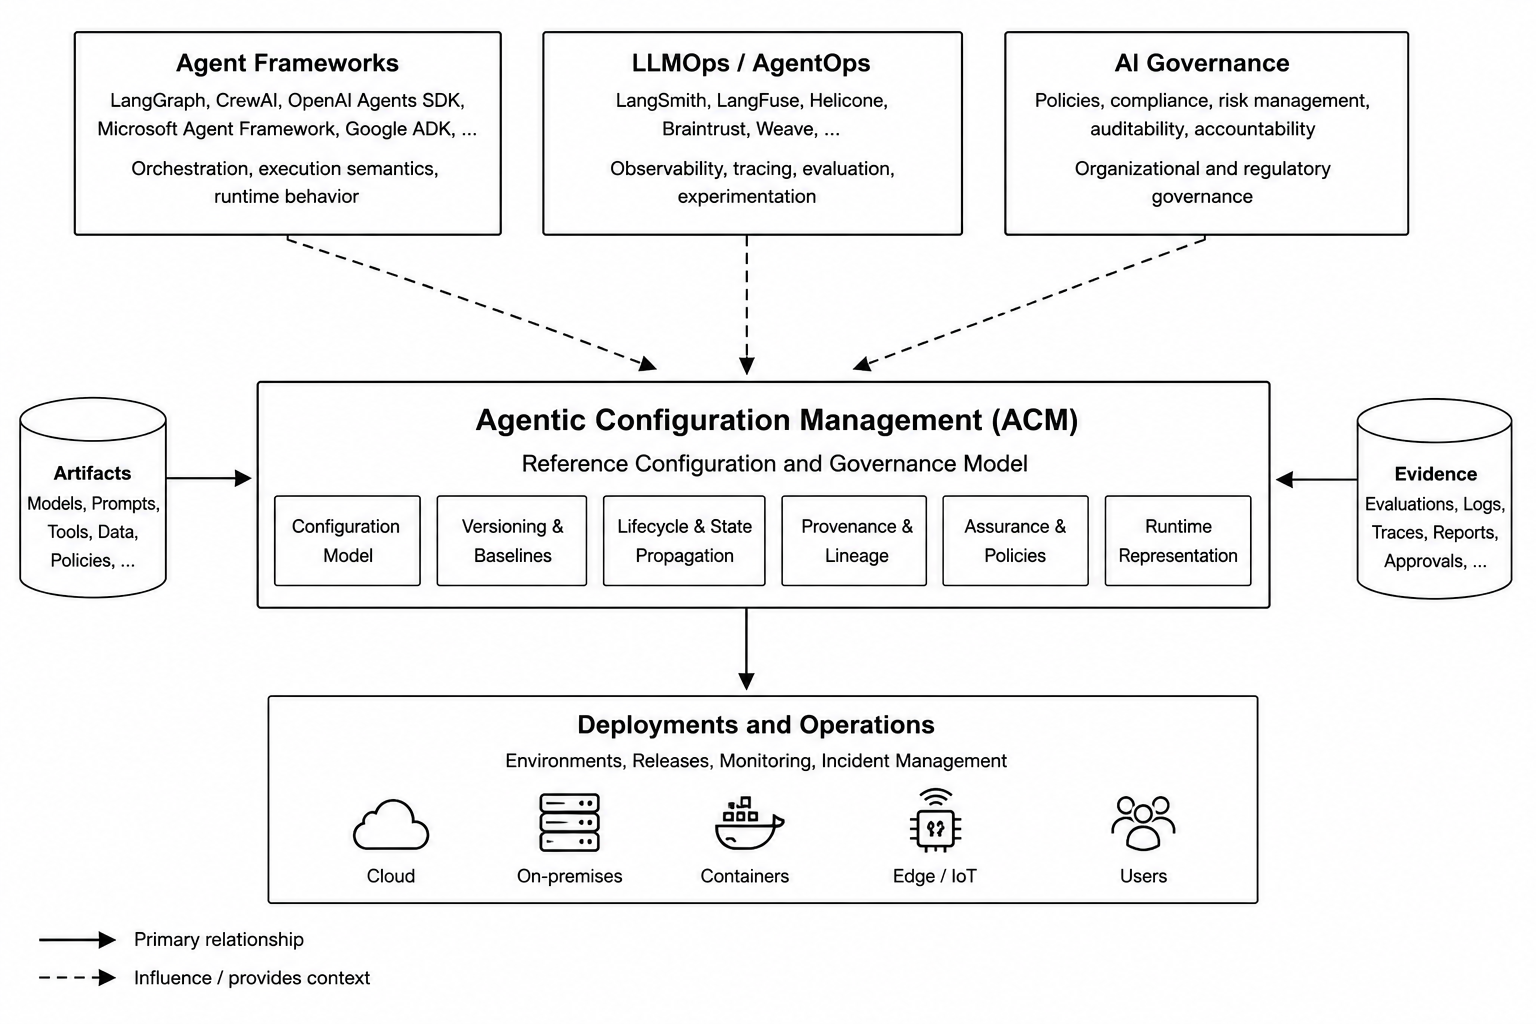
\includegraphics[width=0.7\textwidth]{figures/ACM_architecture_principles.png}
	\caption{Positioning of ACM. ACM acts as a framework-independent configuration layer that connects agent frameworks (orchestration), LLMOps platforms (observability and evaluation) and deployment environments (execution).}
	\label{fig:ACM_positioning}
\end{figure*}

ACM focuses on governing the former while providing formal semantics to interpret the latter relative to the governed configuration. The contributions of this paper are fourfold:

\begin{itemize}
    \item We propose a \textbf{framework-independent governance representation} that defines the core concepts, relationships, and abstractions required to represent governed heterogeneous agentic configurations.
    
    \item We formalize the \textbf{governance semantics} of agentic configurations through lifecycle models, state propagation, assurance semantics, and runtime governance mechanisms.
    
    \item We present a \textbf{reference operationalization} of the model, including a Python reference implementation together with projection mechanisms for heterogeneous agentic frameworks.
    
    \item We evaluate the \textbf{expressiveness and operational feasibility} of the proposed model through normative scenarios, automated validation, quantitative impact analysis and cross-framework projection experiments.
\end{itemize}

The remainder of this paper is organized as follows. Section~\ref{sec:related_work} reviews the foundations of Software Configuration Management, AI governance, LLMOps, AgentOps, and agentic frameworks, and identifies the gap addressed by the Agentic Configuration Model (ACM). Section~\ref{sec:design_principles} derives the design principles of the proposed reference model. Section~\ref{sec:reference_model} introduces the ACM reference model, while Section~\ref{sec:governance_semantics} formalizes its governance semantics. Section~\ref{sec:operationalization} describes its operationalization through a reference architecture, framework adapters, governance algorithms, and a reference implementation. Section~\ref{sec:evaluation} evaluates the proposed model. Finally, Sections~\ref{sec:discussion}, \ref{sec:threats_validity}, \ref{sec:future_work}, and \ref{sec:conclusion} discuss the implications, limitations, future research directions, and conclusions of this work.

\section{Related Work}
\label{sec:related_work}

\subsection{Software Configuration Management}
\label{sec:scm}

Software Configuration Management (SCM) provides the engineering foundations for identifying, controlling, and auditing the evolution of software systems. Rather than focusing solely on version control, SCM defines a disciplined process for establishing configuration baselines, managing change, maintaining traceability, and ensuring that released systems remain reproducible and auditable throughout their lifecycle \cite{whitgift1991methods, conradi1998version, leon2015software, bersoff1984elements, bersoff1978software}.

These principles have been formalized by long-established standards and bodies of knowledge, including IEEE~828, ISO/IEC/IEEE~12207, and the \emph{Software Engineering Body of Knowledge} (SWEBOK) \cite{swebok40, ieee2012ieee, wohlinsnowballing}. Although these references differ in scope, they consistently describe configuration management as a combination of configuration identification, change control, configuration status accounting, and configuration verification and audit.

Classical SCM has proved effective for conventional software systems composed of relatively stable software artifacts such as source code, libraries, documentation, build configurations, and release packages \cite{chacon2014pro}. Its central concepts---configuration items, immutable baselines, controlled revisions, dependency management, and change auditing---provide the foundations required to ensure consistency and reproducibility across software releases.

\begin{figure*}[t]
	\centering
	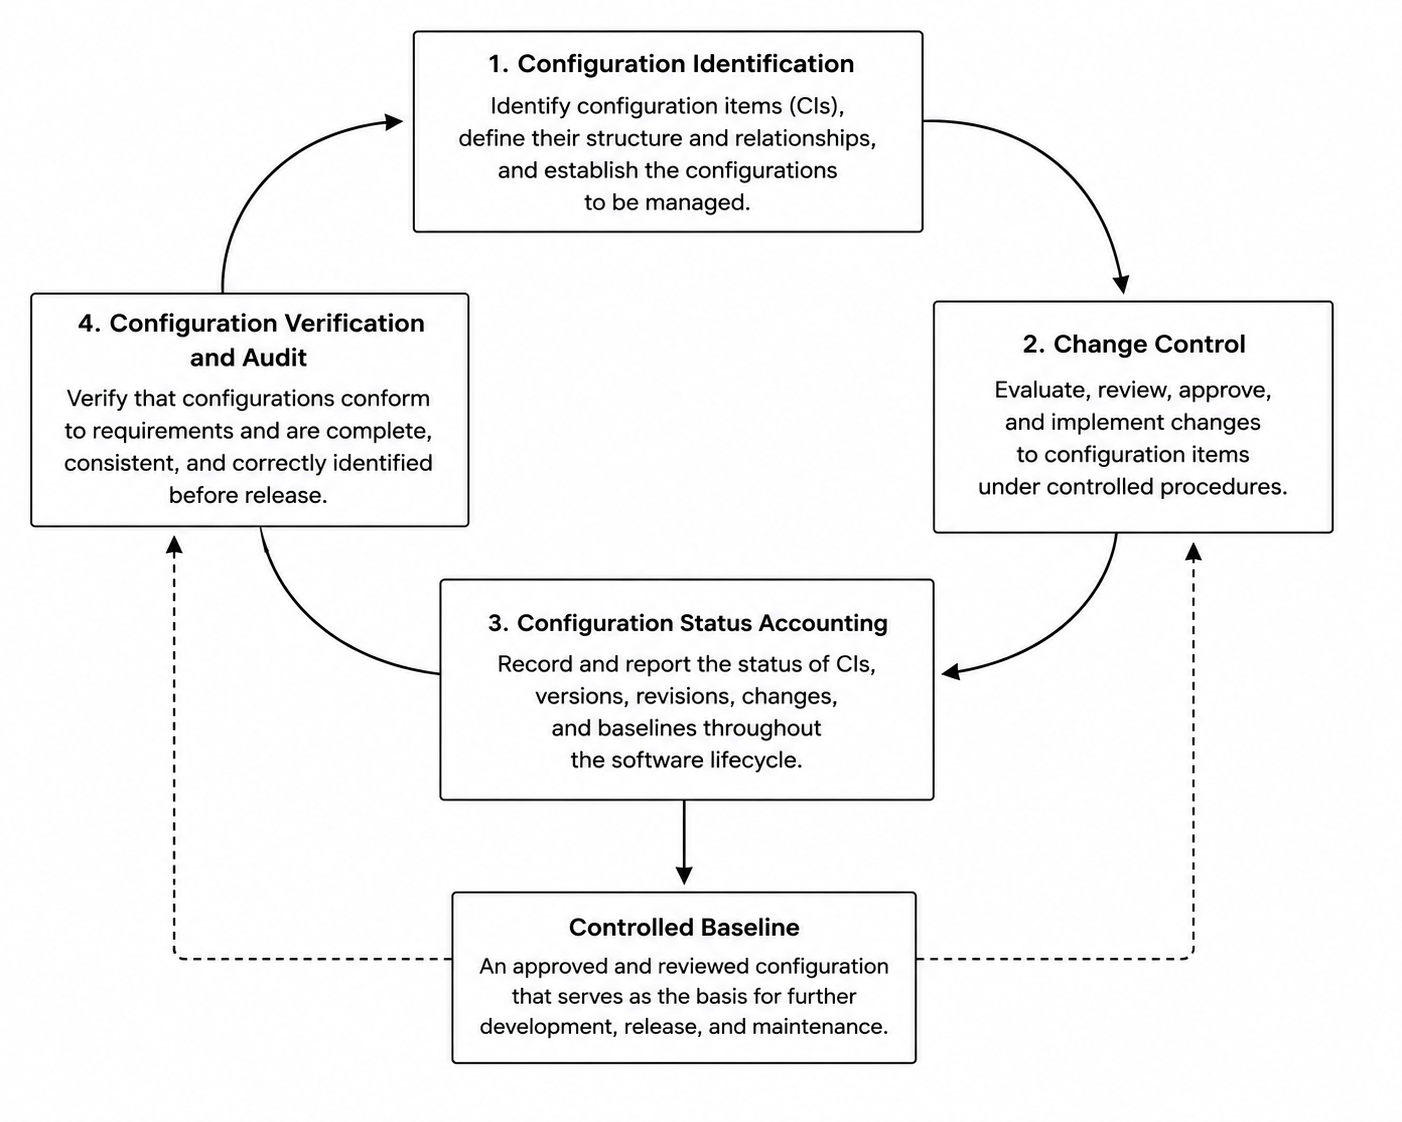
\includegraphics[width=0.7\textwidth]{figures/SCM_configuration_management_liefcycle_baseline.png}
	\caption{Fundamental Software Configuration Management (SCM) process. Configuration identification, change control, configuration status accounting, and configuration verification and audit constitute the four core SCM activities defined by established software engineering standards. Together, they provide the conceptual foundations for immutable revisions, controlled baselines, traceability, and governance that are extended by ACM to heterogeneous agentic systems \cite{bersoff1984elements}.}
	\label{fig:SCM_framework}
\end{figure*}

However, applying these principles directly to agentic systems is not straightforward. In addition to executable software components, agentic systems rely on heterogeneous configurable artifacts, dynamic execution structures, and runtime-generated elements that are not explicitly addressed by traditional SCM models. Consequently, while SCM provides the conceptual foundations for configuration governance, additional abstractions are required to represent and govern the configuration of modern agentic systems.

\subsection{AI Governance}
\label{sec:ai_governance}

The rapid adoption of AI systems has expanded governance concerns beyond traditional software engineering. Recent standards, regulatory frameworks, and technical initiatives emphasize accountability, transparency, risk management, and auditability throughout the AI lifecycle \cite{pandey2025agentic, Engin_Hand_2026, Gangavarapu2025, shavit2023practices, IMDA2026AgenticMGF}. Although these initiatives differ in scope, they share the objective of ensuring that AI systems remain trustworthy, traceable, and subject to appropriate organizational oversight.

From the perspective of agentic systems, three complementary areas are particularly relevant: governance frameworks defining organizational requirements, provenance mechanisms ensuring artifact traceability, and emerging approaches dedicated to the governance of autonomous agents. Together, these perspectives establish important governance objectives but do not define a common configuration representation for heterogeneous agentic systems.

\subsubsection{Governance Frameworks}
\label{sec:governance_frameworks}

Several governance frameworks have established principles for the responsible development and operation of AI systems. Examples include the NIST AI Risk Management Framework (AI RMF), ISO/IEC~42001, ISO/IEC~23894, the OECD AI Principles, and the European AI Act \cite{ai2023artificial, benraouane2024ai, simonetta2024iso, yeung2020recommendation, edwards2021eu}. While their objectives and intended audiences differ, they consistently emphasize governance practices such as accountability, documentation, risk management, human oversight, traceability, and auditability.

These frameworks define organizational objectives and governance processes rather than implementation models. They describe \emph{what} should be governed and documented but intentionally remain independent of the internal representation adopted by AI platforms or execution frameworks. Consequently, they do not provide a framework-independent configuration model capable of representing the complete structure and evolution of an agentic system.

\subsubsection{Provenance and Software Supply Chain}
\label{sec:provenance_supply_chain}

Provenance has become a fundamental requirement for software and AI governance. Existing standards and specifications, including W3C PROV, Software Bills of Materials (SBOMs), SPDX, and the Supply-chain Levels for Software Artifacts (SLSA) \cite{missier2013w3c, SBOM10336262, stewart2010software, okafor2022sok, cobbe2023understanding}, improve traceability by documenting artifact origins, dependencies, integrity, and production processes. These mechanisms strengthen reproducibility, software supply-chain security, and compliance by making software artifacts and their relationships explicitly traceable.

Although highly valuable, these approaches primarily describe software packages, build processes, datasets, or deployment artifacts. They do not represent the semantic configuration of agentic systems, whose behavior depends on heterogeneous configuration artifacts such as agents, prompts, models, skills, composite subsystems, tools, policies, and dynamically evolving execution structures. Consequently, provenance alone is insufficient to govern the configuration of an entire agentic system.

\subsubsection{Governance of Agentic Systems}
\label{sec:agentic_governance}

The emergence of agentic AI has stimulated research on governance mechanisms specifically targeting autonomous and multi-agent systems. Existing approaches typically address runtime supervision, policy enforcement, authorization, monitoring, safety constraints, or operational accountability. Likewise, current AgentOps and orchestration platforms increasingly provide tracing, evaluation, and operational monitoring capabilities for agent execution but are framework-dependent (see Section ~\ref{sec:llmops_agentops}).

This observation complements the limitations identified in classical Software Configuration Management and motivates the need for a unified configuration reference model that separates configuration governance from execution concerns. This gap forms the foundation of the Agentic Configuration Management (ACM) reference model introduced in the following sections.

\subsection{LLMOps and AgentOps}
\label{sec:llmops_agentops}

The emergence of large language models has also given rise to a new generation of operational platforms dedicated to managing AI applications throughout their lifecycle. Inspired by established MLOps practices, LLMOps extends operational support to applications built around foundation models by providing capabilities for prompt management, experimentation, evaluation, deployment, monitoring, and observability. As agentic systems have become increasingly dynamic and autonomous, these practices have naturally evolved toward AgentOps, which addresses the operational management of multi-agent applications and long-running agentic workflows \cite{cesarano2026grand, shavit2023practices, pandey2025agentic, dumas2026}.

Unlike traditional software configuration management, LLMOps and AgentOps focus primarily on the operational lifecycle of AI applications rather than on the governance of their underlying configurations \cite{pahune2025transitioning, amershi2019, dong2024agentops}. Their objective is to facilitate development, deployment, monitoring, experimentation, and continuous improvement while maintaining visibility over system behavior during execution.

Although terminology varies across platforms, most LLMOps and AgentOps solutions converge toward a common set of operational capabilities, including prompt management, execution tracing, evaluation workflows, observability, deployment management, and experiment tracking. These capabilities provide the operational evidence required to understand how an AI application behaves in production and to support iterative improvements of prompts and workflows.

From the perspective of configuration governance, several concepts introduced by these platforms are particularly relevant. 

\begin{itemize}
	\item Configuration management concerns the explicit representation of configurable artifacts and their versions \cite{liu2025towards, Hughes03072025, langfusedocs, heliconedocs}. 
	\item Provenance records the origin and derivation history of these artifacts.
	\item Lineage captures the dependency relationships connecting successive versions, execution traces, and derived artifacts \cite{cesarano2026grand, rajath2025review}. 
	\item Tracing records the sequence of execution events occurring during system operation.
	\item Observability \cite{langsmithdocs} aggregates telemetry that enables operators to inspect the internal behavior of deployed applications \cite{opentelemetry}. 
	\item Deployment state characterizes the operational status of a configuration once deployed within a target environment \cite{braintrustdocs}.
\end{itemize}	

These concepts constitute essential building blocks for governing modern AI applications. However, they generally remain attached to operational artifacts such as prompts, traces, evaluations, or deployments, rather than providing a unified representation of the complete configuration of an agentic system. Relationships among agents, prompts, models, tools, skills, composite subsystems, policies, workflows, and runtime-generated components are typically represented through platform-specific abstractions, preventing the establishment of a framework-independent configuration model.

Representative platforms illustrate this evolution. Prompt management solutions increasingly support prompt versioning, labels, rollback, experimentation, and deployment workflows. Observability platforms provide execution traces, telemetry, evaluation pipelines, and runtime analytics. More recent AgentOps environments extend these capabilities to multi-agent executions through richer runtime monitoring, workflow inspection, and execution replay \cite{sahir2026agentops}. 

As an example of open-source observability platform, we can cite LangFuse~\cite{langfusedocs} providing prompt management, execution tracing, evaluation, experimentation, and prompt versioning. It enables developers to associate prompt revisions with runtime traces, datasets, and evaluation results, thereby improving reproducibility and experimentation across LLM-based applications. 
Another observability platform is Helicone ~\cite{heliconedocs}. It supports request tracing, prompt versioning, experimentation, evaluation, and deployment management. Its primary focus is operational monitoring and prompt-centric development workflows, providing valuable runtime telemetry and performance insights. 

Together, these platforms substantially improve the operational governance of AI applications but remain centered on execution management rather than on the governance of configuration itself, nevertheless they do no aim at representing the complete configuration of heterogeneous agnetic system (see Table ~\ref{tab:llmops_comparison} for a governance capability comparison between the current LLMOPs and AgentOps platforms).

\begin{table*}[t]
\centering
\caption{Representative capabilities of current LLMOps and AgentOps platforms. The comparison highlights their primary focus on operational lifecycle management rather than framework-independent configuration governance.}
\label{tab:llmops_comparison}

\renewcommand{\arraystretch}{1.15}
\begin{tabular}{p{4.2cm}ccccc}
\toprule
\textbf{Capability} &
\textbf{LangSmith} &
\textbf{LangFuse} &
\textbf{Helicone} &
\textbf{Braintrust} &
\textbf{PromptLayer} \\
\midrule

Prompt versioning                & \checkmark & \checkmark & \checkmark & \checkmark & \checkmark \\

Prompt deployment / labels       & $\sim$ & \checkmark & \checkmark & $\sim$ &  \checkmark \\

Execution tracing                & \checkmark & \checkmark & \checkmark & \checkmark & \checkmark \\

Observability / telemetry        & \checkmark & \checkmark & \checkmark & \checkmark & $\sim$ \\

Evaluation workflows             & \checkmark & \checkmark & \checkmark & \checkmark & $\sim$ \\

Experiment tracking              & \checkmark & \checkmark & \checkmark & \checkmark & $\sim$ \\

Prompt provenance                & $\sim$ & \checkmark & \checkmark & $\sim$ & \checkmark \\

Execution lineage                & \checkmark & \checkmark & \checkmark & \checkmark & $\sim$ \\

Deployment state                 & $\sim$ & \checkmark & \checkmark & $\sim$ & \checkmark \\

Runtime replay                   & \checkmark & $\sim$ & $\sim$ & $\sim$ & $\sim$ \\

Framework-specific integrations  & \checkmark & \checkmark & \checkmark & \checkmark & \checkmark \\

\midrule

Framework-independent configuration model
                                 & -- & -- & -- & -- & -- \\

Configuration graph              & -- & -- & -- & -- & -- \\

Immutable configuration baseline & -- & -- & -- & -- & -- \\

Configuration lifecycle          & -- & -- & -- & -- & -- \\

Configuration dependency model   & -- & -- & -- & -- & -- \\

Governed configuration revisions & -- & -- & -- & -- & -- \\

Configuration state propagation  & -- & -- & -- & -- & -- \\

Configuration governance semantics
                                 & -- & -- & -- & -- & -- \\

\bottomrule
\end{tabular}

\vspace{1mm}

\footnotesize
$\checkmark$ Supported \hspace{1em}
$\sim$ Partial support \hspace{1em}
-- Not provided as a first-class capability.

\end{table*}

\subsection{Agentic Frameworks}
\label{sec:agentic_frameworks}

The rapid adoption of agentic AI has led to the emergence of numerous frameworks dedicated to designing and executing autonomous or multi-agent applications. Although their architectures differ, these frameworks share a common objective: orchestrating the execution of agents, coordinating interactions among heterogeneous components, and integrating large language models with external tools, memory, and user-defined workflows (non exhaustive list of frameworks \cite{crewaidocs, langgraphdocs, googleadkdocs, microsoftadkdocs, openaiddocs, claudedocs, mistraldocs}).

Current frameworks cover a broad spectrum of orchestration paradigms. Some adopt explicit graph-based execution models, while others organize applications around agents, tasks, crews, or conversational interactions. Despite these architectural differences, they generally provide abstractions for defining execution flows, invoking tools, managing shared or local state, and coordinating agent interactions during runtime (see Table ~\ref{tab:framework_comparison} in Appendix ~\ref{appendix:related_work}).

Beyond execution, modern frameworks increasingly incorporate operational capabilities such as checkpointing, persistence, human-in-the-loop interactions, execution replay, and integration with observability platforms. These features considerably simplify the development and deployment of agentic applications and complement the operational services provided by LLMOps and AgentOps platforms.

However, the internal representations adopted by these frameworks remain closely coupled to their respective execution models. Configuration artifacts, dependency structures, lifecycle conventions, and runtime abstractions are expressed through framework-specific concepts that are not directly interoperable. Consequently, while these frameworks provide rich execution semantics, they do not define a common representation suitable for governing configurations independently of a particular execution environment.



\subsection{Gap Analysis}
\label{sec:gap_analysis}

The preceding sections have examined complementary perspectives on the governance of AI systems, including Software Configuration Management, AI governance frameworks, LLMOps and AgentOps platforms, and agentic execution frameworks. Although these approaches address different aspects of the AI lifecycle, they collectively contribute to the governance of modern AI applications. However, they cannot simply be combined to obtain a unified configuration-governance solution. Software Configuration Management governs software artifacts but has no framework-independent representation of agentic abstractions. AI governance frameworks define organizational objectives and compliance requirements without specifying a configuration model. LLMOps and AgentOps platforms provide observability, evaluation, and operational tooling, while execution frameworks define runtime semantics through framework-specific abstractions. 

Because each family addresses a different governance concern and relies on its own representation of the system, no common semantic model exists for representing, versioning, and governing heterogeneous agentic configurations independently of their execution environment.
This observation motivates the need for a framework-independent reference configuration model capable of integrating these complementary perspectives while preserving a stable governance representation across heterogeneous agentic ecosystems.

Table~\ref{tab:gap_analysis} synthesizes the coverage of representative governance capabilities across these complementary families of approaches. Rather than comparing the approaches themselves, the analysis evaluates the extent to which each family addresses the governance capabilities required throughout the lifecycle of agentic systems.

\begin{table*}[t]
\centering
\caption{Coverage of representative governance capabilities across complementary families of approaches. A detailed comparison is provided in Appendix Table ~\ref{tab:gap_analysis_detailed}.}
\label{tab:gap_analysis}

\renewcommand{\arraystretch}{1.15}

\begin{tabular}{p{5.2cm}ccccc}
\toprule
\textbf{Governance Capability}
&
\textbf{SCM}
&
\textbf{AI Gov.}
&
\textbf{LLMOps / AgentOps}
&
\textbf{Frameworks}
\\
\midrule

Configuration identification          & \checkmark & $\sim$ & $\sim$ & $\sim$ \\

Version management                    & \checkmark & -- & $\sim$ & $\sim$ \\

Configuration provenance              & $\sim$ & \checkmark & \checkmark & $\sim$ \\

Dependency traceability               & \checkmark & $\sim$ & \checkmark & $\sim$ \\

Execution observability               & -- & $\sim$ & \checkmark & \checkmark \\

Lifecycle governance                  & $\sim$ & \checkmark & $\sim$ & $\sim$ \\

Framework-independent representation  & -- & -- & -- & -- \\

Unified configuration model           & -- & -- & -- & -- \\

\bottomrule
\end{tabular}

\vspace{1mm}

\footnotesize
$\checkmark$ Fully addressed \hspace{1em}
$\sim$ Partially addressed \hspace{1em}
-- Not addressed as a primary capability.

\end{table*}

The limitation of combining these approaches is therefore not the absence of governance, observability, execution, or compliance mechanisms. Rather, these capabilities remain distributed across complementary technologies that operate on different abstractions and representations. As a result, governed configurations cannot be represented, versioned, compared, and evolved through a common semantic model independently of the underlying execution framework. Our reference model ACM addresses this missing abstraction layer by introducing a framework-independent reference configuration model that unifies configuration governance while remaining complementary to existing execution frameworks, LLMOps platforms, AgentOps solutions, and organizational AI governance frameworks. These observations provide the rationale for designing a unified reference model which is presented in the next section. It establishes the requirements for a unified reference model dedicated to configuration governance for agentic systems (see next Section ~\ref{sec:design_principles}).

\section{Design Principles}
\label{sec:design_principles}

Rather than extending an existing orchestration framework or operational platform, the objective of ACM is to establish a reference model that complements these ecosystems while remaining independent of their implementation technologies. ACM addresses therefore a complementary concern by representing governed configurations independently of execution platforms, enabling immutable baselines, dependency-aware configuration management, and explicit relationships between configuration revisions, runtime observations, and assurance evidence.

The design of such a reference model is guided by a set of requirements derived from the limitations identified in the preceding analysis. These principles define the properties that any framework-independent configuration governance model should satisfy. They intentionally describe design requirements rather than implementation choices; the conceptual realization of these principles is introduced in Section~\ref{sec:reference_model}.

Table~\ref{tab:design_principles} summarizes the seven principles that guide the design of ACM.
\begin{table*}[t]
\centering
\caption{Design principles guiding the ACM reference model.}
\label{tab:design_principles}

\renewcommand{\arraystretch}{1.15}

\begin{tabular}{p{1.0cm}p{4.0cm}p{9.2cm}}
\toprule
\textbf{ID} &
\textbf{Principle} &
\textbf{Objective}
\\
\midrule

P1 &
Framework Independence &
Remain independent of execution frameworks, orchestration engines, and AI providers.\\

P2 & Explicit Configuration Representation & Represent every configurable artifact explicitly under configuration governance.\\

P3 &  Immutable Versioning & Ensure deterministic evolution through immutable revisions and controlled baselines. \\

P4 & Configuration–Execution Separation & Clearly distinguish governed configurations from runtime execution.\\

P5 & Explicit Traceability & Preserve provenance and dependency relationships throughout the configuration lifecycle.\\

P6 & Governance by Design & Support lifecycle governance, policy enforcement, assurance, and auditability.\\

P7 & Extensibility & Allow the reference model to evolve without changing its governance foundations.
\\
\bottomrule
\end{tabular}

\end{table*}

\paragraph{P1 -- Framework Independence}

A configuration governance model shall remain independent of any specific orchestration framework, execution engine, or AI provider. Heterogeneous agentic systems should therefore be representable through a common abstraction that preserves governance semantics without exposing framework-specific implementation details. This independence enables interoperability across evolving ecosystems while avoiding dependence on a particular execution technology.

\paragraph{P2 -- Explicit Configuration Representation}

Every artifact whose definition influences the behaviour of an agentic system shall be represented explicitly as a governed configuration object. The model should support heterogeneous artifacts while remaining independent of their implementation and execution semantics.

\paragraph{P3 -- Immutable Versioning}

Configuration evolution shall rely on immutable revisions. Every modification shall produce a new governed revision while preserving previous versions to ensure reproducibility, auditability, and deterministic reconstruction of historical configurations.

\paragraph{P4 -- Configuration--Execution Separation}

Configuration governance shall remain conceptually independent from runtime execution. Runtime observations may enrich governance information but shall not directly modify governed configurations.

\paragraph{P5 -- Explicit Traceability}

The model shall preserve explicit traceability among governed artifacts throughout their lifecycle. Structural dependencies, provenance relationships, and configuration evolution should remain observable and auditable independently of any execution framework.

\paragraph{P6 -- Governance by Design}

Governance shall be an intrinsic property of the configuration model rather than an external operational concern. The model should support lifecycle control, policy evaluation, assurance, auditability, and deterministic governance decisions.

\paragraph{P7 -- Extensibility}

The reference model shall remain extensible to accommodate future categories of configuration artifacts, governance policies, and execution paradigms without modifying its fundamental governance principles.


The following section introduces the ACM reference model, which operationalizes these principles through a normalized representation of governed configuration artifacts and their relationships.

\section{ACM Reference Model}
\label{sec:reference_model}

The ACM is made to offer a common governance layer capable of representing heterogeneous configuration artifacts independently of their execution environment.

The model is designed around three complementary objectives. First, it provides a unified representation of configurable artifacts participating in an agentic system. Second, it explicitly captures the structural and governance relationships among these artifacts. Third, it establishes the conceptual foundations required to support lifecycle management, traceability, provenance, auditability, and configuration evolution.

Section~\ref{sec:conceptual_overview} introduces the conceptual organization of the model. Section~\ref{sec:aci_model} defines the abstract representation of Agentic Configuration Items (ACIs). The following subsections specify the relationships between ACIs, baseline composition, and the structural properties of the reference model.


\subsection{Conceptual Overview}
\label{sec:conceptual_overview}

An agentic system is composed of numerous configurable artifacts originating from heterogeneous technologies, including orchestration frameworks, language models, prompts, tools, skills, composite subsystems, policies, execution environments, and governance mechanisms. Although these artifacts collectively determine the behaviour of the system, they are generally represented through framework-specific abstractions and governed independently.

The ACM reference model introduces a unified conceptual representation in which every configurable artifact is treated as a governed configuration item, regardless of its implementation technology or execution framework. This abstraction enables heterogeneous artifacts to be managed according to a common governance model while preserving their individual semantics.

Rather than organizing configuration items according to implementation technologies, ACM structures them according to the governance role they fulfil within the system. Configuration items are therefore organized into three conceptually independent families:

\begin{itemize}

\item \textbf{Structural items}, which describe the static composition of the system and its configurable artifacts.

\item \textbf{Governance items}, which define policies, assurance evidence, compliance constraints, and lifecycle governance.

\item \textbf{Runtime items}, which represent execution-related information generated during system operation while remaining linked to the governed configuration.

\end{itemize}

Although these families are conceptually independent, they remain connected through explicit relationships that preserve traceability across the complete lifecycle of the system. This organization separates structural configuration, governance information, and runtime observations while allowing each perspective to evolve independently.

To represent these complementary perspectives, ACM organizes configuration information into four interconnected conceptual graphs, illustrated in Figure~\ref{fig:acm_reference_model}.

Formally, the ACM reference model is represented as the ordered multi-graph structure

\begin{equation}
	\mathcal{G}_{\mathrm{ACM}}
	=
	\left(
	G_C,
	G_E,
	G_A,
	G_R
	\right),
	\label{eq:acm_multigraph_structure}
\end{equation}

where $G_C$, $G_E$, $G_A$, and $G_R$ denote the Configuration, Evolution, Assurance, and Runtime Graphs, respectively. The four graphs represent distinct governance views and remain connected through explicit relationships and revision-level provenance.

\begin{itemize}

\item The \textbf{Configuration Graph} represents the governed configuration of the agentic system and the structural relationships among configuration items.

\item The \textbf{Assurance Graph} captures governance policies, assurance evidence, compliance constraints, and policy enforcement.

\item The \textbf{Runtime Graph} represents execution observations generated during system operation while maintaining explicit links to governed configuration items.

\item The \textbf{Evolution Graph} provides an integrated view of configuration evolution and history from a baseline.

\end{itemize}

The decomposition into four complementary graphs is a deliberate design decision rather than a modeling convenience. Each graph addresses a distinct governance concern that follows its own semantics and lifecycle. Separating these orthogonal concerns preserves conceptual clarity, avoids mixing static and dynamic governance information, and enables each graph to evolve independently while remaining linked through explicit traceability relationships. 

\begin{figure*}[t]
	\centering
	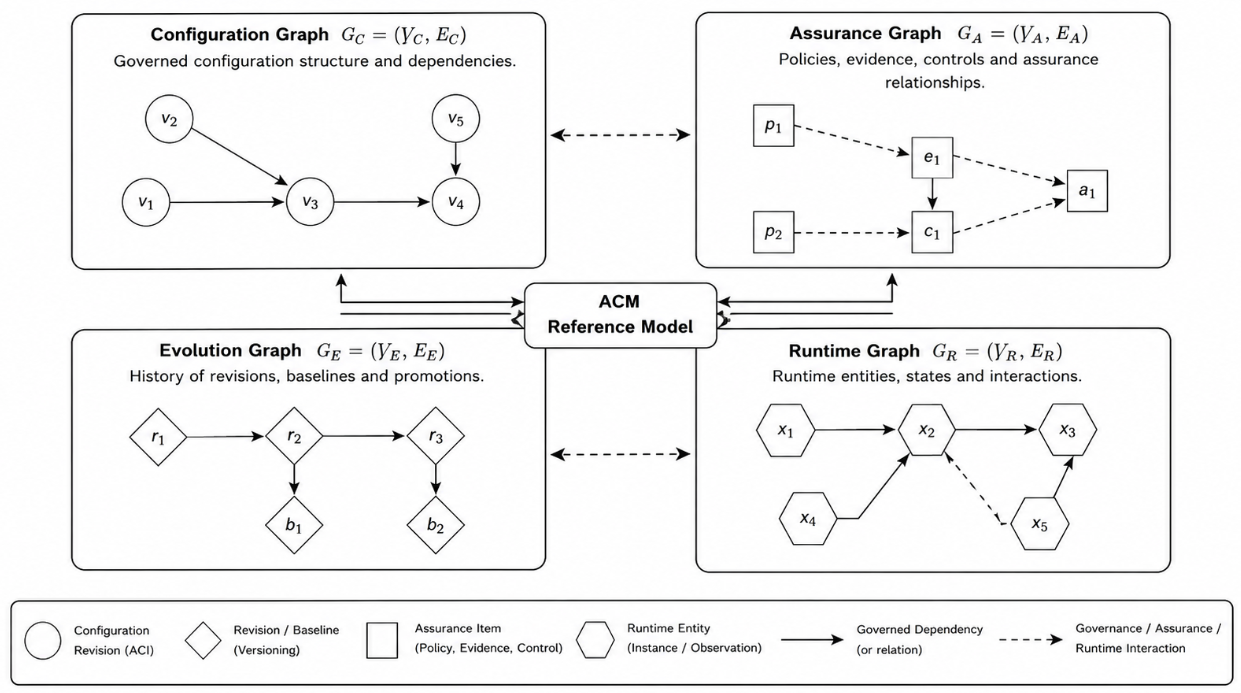
\includegraphics[width=0.6\textwidth]{figures/ACM_reference_model.png}
	\caption{Multi-graph organization of the ACM reference model. Configuration, evolution, runtime, and assurance are represented as four complementary governance views linked through immutable configuration revision and explicit provenance relationships.}
	\label{fig:acm_reference_model}
\end{figure*}

\subsection{Agentic Configuration Item}
\label{sec:aci_model}

The Agentic Configuration Item (ACI) is the fundamental abstraction of the ACM reference model. An ACI represents any configurable artifact whose definition contributes to the specification, governance, or execution of an agentic system. By introducing a common abstraction independent of implementation technologies, ACM enables heterogeneous artifacts originating from different frameworks to be represented and governed uniformly.

Unlike traditional software configuration items, which primarily describe software artifacts, ACIs encompass the broader range of configurable elements required by modern agentic systems. Examples include agents, prompts, skills, composite subsystems, workflows, tools, language models, policies, assurance evidence, runtime observations, and other governance artifacts. Although these artifacts differ in purpose and lifecycle, they share a common representation within the ACM reference model (see Figure ~\ref{fig:aci_metamodel}).

Every ACI is represented as an immutable configuration revision. Once created, the content associated with a revision never changes; any modification results in the creation of a new revision while preserving previous versions for reproducibility, auditability, and deterministic reconstruction of historical configurations. Configuration evolution is therefore represented explicitly through successive governed revisions rather than mutable objects.

An ACI combines three complementary dimensions:

\begin{itemize}

\item an immutable configuration content describing the governed artifact;

\item an identity and revision model ensuring uniqueness, version management, and reproducibility;

\item governance metadata describing lifecycle information, provenance, integrity, and other management attributes required for configuration governance.

\end{itemize}

This representation intentionally separates the conceptual identity of a configuration item from the successive revisions describing its evolution. A configuration item therefore exists independently of any particular revision, while each revision represents a complete immutable state of that item at a specific point in its lifecycle.

To accommodate the diversity of configurable artifacts encountered in agentic systems, ACIs are organized into three conceptually independent families introduced in Section~\ref{sec:conceptual_overview}: Structural ACIs, Governance ACIs, and Runtime ACIs. These families share the same abstract representation while specializing the governed content according to the role performed by each artifact within the reference model. This specialization enables the model to remain extensible without introducing family-specific governance mechanisms.

Figure~\ref{fig:aci_metamodel} presents the abstract representation of an Agentic Configuration Item. The following subsections specify its attributes, relationships, and composition rules.

\begin{figure*}[t]
	\centering
	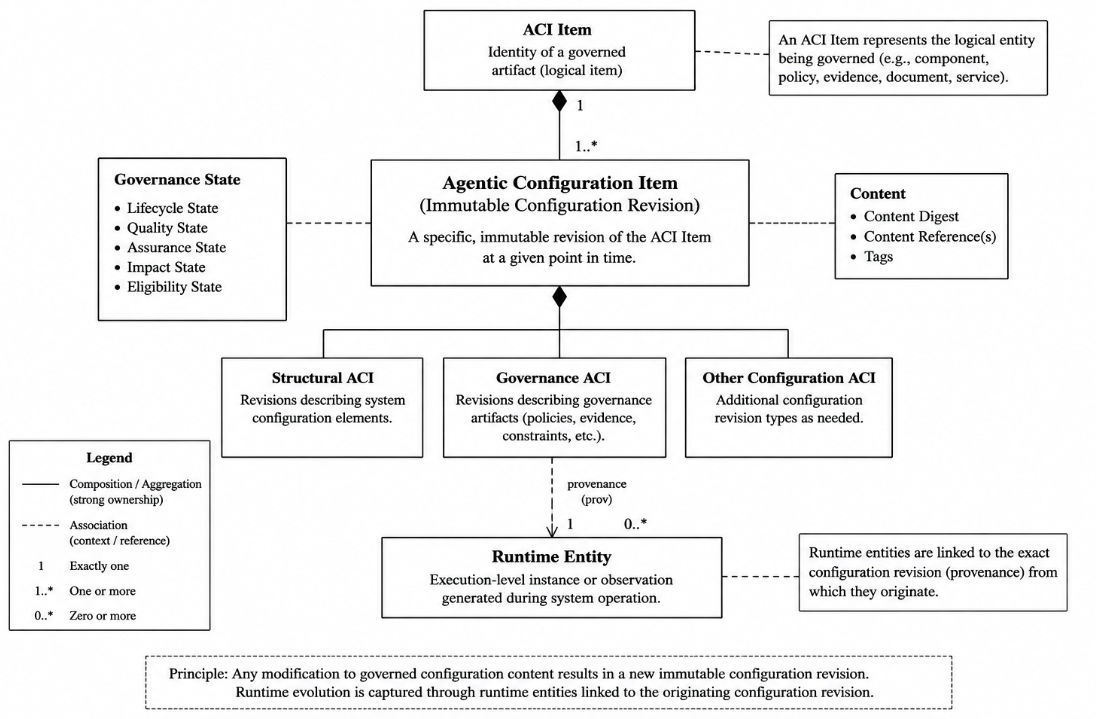
\includegraphics[width=\textwidth]{figures/ACI_metamodel_old.png}
	\caption{Metamodel of the Agentic Configuration Item (ACI). The ACI constitutes the fundamental building block of the ACM reference model. The metamodel defines a common representation for governed configuration items, their specialization hierarchy (Structural, Governance, and Runtime ACIs), agentic configuration types, and governance metadata. Associated entities, including provenance records, content digests, content references, and tags, provide the information required for immutable identification, traceability, integrity verification, and reproducible configuration management.}
	\label{fig:aci_metamodel}
\end{figure*}

\subsection{ACI Representation}
\label{sec:configuration_item_representation}

The abstract representation introduced in the previous section is realized through a normalized set of attributes shared by all Agentic Configuration Items, regardless of their specialization. This common representation provides a consistent governance model while allowing individual artifact categories to define their own domain-specific content.

The representation of an ACI is organized into four complementary components:

\begin{itemize}

\item \textbf{Identity}, uniquely identifying both the configuration item and the immutable revision to which the representation corresponds.

\item \textbf{Governance state}, describing the lifecycle, quality, compliance, and assurance status associated with the revision.

\item \textbf{Configuration content}, containing the governed artifact together with integrity information and extensible metadata.

\item \textbf{Governance metadata}, recording provenance, user-defined properties, and additional information required for lifecycle management and auditing.

\end{itemize}

This separation isolates the immutable content of a configuration revision from the metadata required to govern its evolution. Consequently, governance information may evolve independently from the business semantics of individual artifact categories while preserving the integrity of immutable revisions.

Table~\ref{tab:aci_attributes} summarizes the attributes composing the abstract representation of an ACI.

\begin{table*}[t]
\centering
\caption{Abstract attributes of an Agentic Configuration Item revision.}
\label{tab:aci_attributes}

\renewcommand{\arraystretch}{1.15}

\begin{tabular}{p{3.3cm}p{3.4cm}p{8.3cm}}

\toprule

\textbf{Category} &
\textbf{Representative Attributes} &
\textbf{Purpose}

\\
\midrule

Identity &
item\_id, revision\_id &
Uniquely identify the governed item and its immutable revision.

\\

Governance State &
lifecycle\_state, quality\_state, assurance\_state, compliance\_state &
Describe the governance status of the revision.

\\

Configuration Content &
content, digest, metadata &
Represent the governed artifact together with integrity and extensible descriptive information.

\\

Governance Metadata &
provenance, tags, custom properties &
Support traceability, auditing, provenance, and organization-specific extensions.

\\

\bottomrule

\end{tabular}

\end{table*}

Although every ACI shares this common representation, the interpretation of the governed content depends on the specialization of the configuration item. Structural, Governance, and Runtime ACIs therefore reuse the same abstract representation while encapsulating different categories of governed artifacts.

\subsection{Relationship Model}
\label{sec:configuration_relationships}

Individual configuration items do not exist in isolation. The complete configuration of an agentic system emerges from the explicit relationships connecting governed artifacts across structural, governance, and runtime perspectives. These relationships constitute the semantic backbone of the ACM reference model by preserving dependency information independently of any execution framework.

Unlike conventional orchestration frameworks, where relationships are often embedded within implementation-specific structures, ACM represents relationships as explicit governed entities. This representation enables dependency analysis, impact assessment, provenance tracking, and configuration validation to be performed independently of execution technologies.

ACM distinguishes several categories of relationships according to their governance semantics:

\begin{itemize}

\item \textbf{Configuration relationships} describe the composition and dependency structure of governed configuration items.

\item \textbf{Assurance relationships} associate configuration items with policies, assurance evidence, compliance requirements and ownership.

\item \textbf{Runtime relationships} connect execution observations to the governed configuration from which they originate.

\item \textbf{Evolution relationships} preserve provenance, revision lineage, and derivation history.

\end{itemize}

Each relationship is explicitly typed and directional. Relationship types define their admissible source and target configuration items together with the semantic constraints governing their interpretation. This explicit typing allows validation rules to be evaluated independently from artifact implementations while ensuring consistent dependency semantics across heterogeneous agentic systems.

Figure~\ref{fig:relationship_model} illustrates the conceptual organization of relationship categories within the ACM reference model.
\begin{figure*}[t]
	\centering
	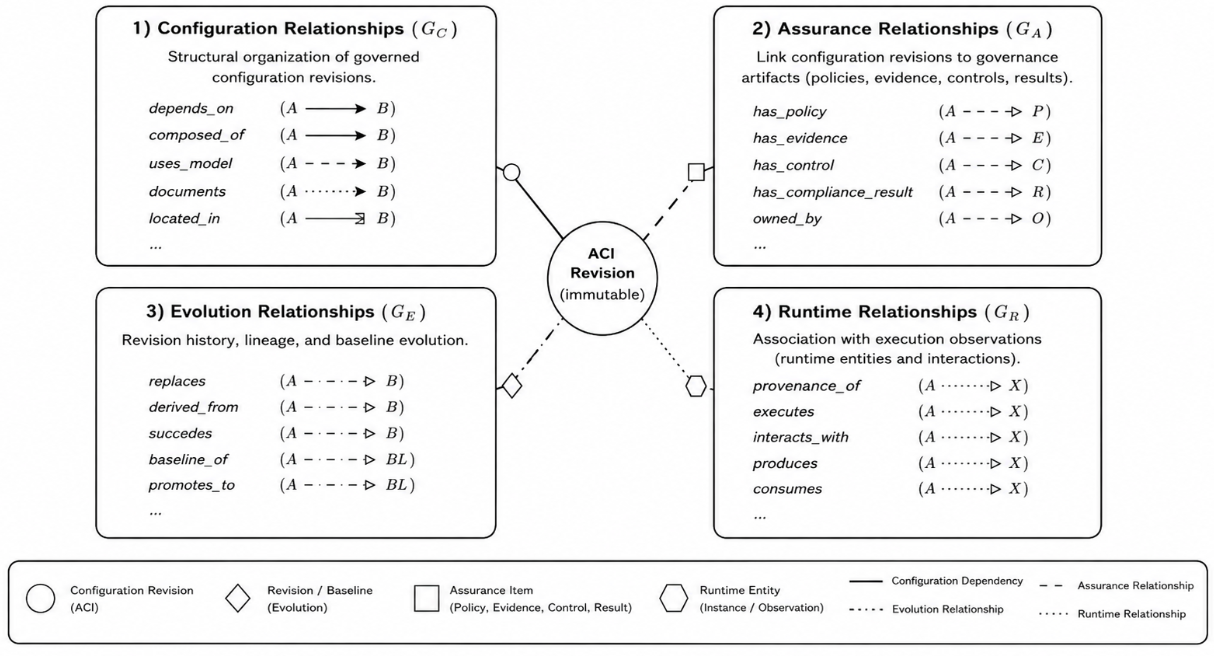
\includegraphics[width=0.6\textwidth]{figures/aci_relationship.png}
	\caption{Relationship categories associated with an immutable \textit{ACI Revision}. ACM organizes relationships into four complementary families aligned with the governance views of the reference model. Configuration relationships describe the structural organization of governed configuration items, Evolution relationships capture revision history and baseline evolution, Runtime relationships associate immutable revisions with execution observations, and Assurance relationships link configuration revisions to governance evidence, compliance results, and policy enforcement. This categorization separates orthogonal governance concerns while preserving explicit traceability through a common immutable revision.}
	\label{fig:relationship_model}
\end{figure*}

\subsection{Release Baselines}
\label{sec:release_baselines}

While Agentic Configuration Items represent individual governed artifacts, operational deployments require a consistent representation of complete system configurations. ACM introduces the notion of a \emph{Release Baseline} to capture a coherent and reproducible snapshot of an agentic system at a specific point in its evolution.

A Release Baseline is an immutable collection of ACI revisions that collectively define the governed configuration of an agentic system. Rather than referencing configuration items independently of their evolution, a baseline always references specific immutable revisions, ensuring that the complete configuration can be reconstructed \emph{deterministically} at any time.

The purpose of a Release Baseline extends beyond simple version aggregation. It establishes the governance boundary within which configuration consistency, traceability, compliance, and assurance can be evaluated. Consequently, governance decisions are performed on complete configurations rather than on isolated artifacts whenever system-wide consistency is required.

A Release Baseline is characterized by the following properties:

\begin{itemize}

\item it references immutable revisions rather than mutable configuration items;

\item it represents a complete and internally consistent governed configuration;

\item it preserves all structural, governance, runtime, and traceability relationships among referenced artifacts;

\item it constitutes the primary unit for reproducibility, audit, release management, and compliance assessment.

\end{itemize}

Baselines are themselves governed configuration objects. They possess their own identity, lifecycle, provenance, and governance metadata while remaining immutable after publication. The evolution of a system is therefore represented as a sequence of immutable Release Baselines, each corresponding to a governed configuration state.

Because every baseline references immutable ACI revisions, historical configurations remain reproducible even when individual configuration items continue to evolve. This property enables deterministic reconstruction, historical audits, rollback, and longitudinal analysis without modifying previously released configurations.

Figure~\ref{fig:release_baseline} illustrates the conceptual organization of a Release Baseline and its relationship with the governed configuration items composing an agentic system.
\begin{figure*}[t]
	\centering
	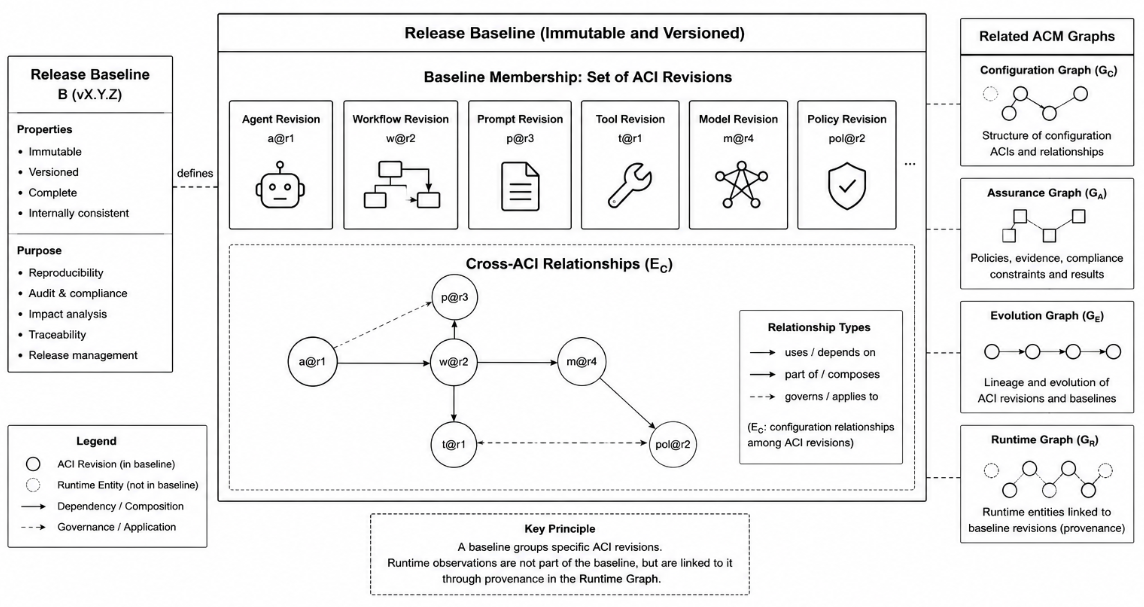
\includegraphics[width=\textwidth]{figures/release_baseline.png}
	\caption{Conceptual organization of an ACM release baseline. A release baseline defines an immutable and versioned snapshot of the governed configuration by grouping a consistent set of ACI revisions. Baseline membership explicitly identifies the configuration revisions composing the release, while cross-ACI relationships preserve the structural dependencies among configuration items (e.g., agents, workflows, prompts, tools, models, and policies). This separation allows a baseline to provide a reproducible configuration snapshot while maintaining the dependency information required for impact analysis, traceability, and governance throughout the system lifecycle.}
	\label{fig:release_baseline}
\end{figure*}

\section{Governance Semantics}
\label{sec:governance_semantics}

The ACM reference model specifies the structural organization of governed agentic systems. This section complements the metamodel by defining the operational semantics governing lifecycle evolution, state evaluation, dependency propagation, and runtime reconstruction.

The governance semantics are intentionally defined independently from any execution framework. Their purpose is not to describe execution behavior but to provide a deterministic interpretation of governed configurations throughout their lifecycle.

Let

\begin{equation}
	G_C=(V_C,E_C)
	\label{eq:configuration_graph}
\end{equation}

denote the ACM Configuration Graph, where $V_C$ is the finite set of immutable ACI revisions represented in the governed configuration and
$E_C$ is the finite set of typed configuration relationships between these revisions.

Each configuration revision $v\in V_C$ is associated with an intrinsic
configuration governance descriptor

\begin{equation}
	\Gamma_C(v)=
	\left(
	L(v),
	Q(v),
	A(v),
	I(v),
	El(v)
	\right),
	\label{eq:governance_descriptor}
\end{equation}

where the individual components respectively denote the lifecycle, quality, assurance, impact, and eligibility states associated with revision $v$.
Runtime state is defined separately on runtime entities and is related to configuration revisions through provenance.
For the same configuration revision, the runtime view is defined as

\begin{equation}
	\rho(v)
	=
	\left\{
	(x,Rt(x))
	\mid
	x\in V_R,\;
	prov(x)=v
	\right\},
	\label{eq:runtime_view}
\end{equation}

where $V_R$ denotes the set of runtime entities,
$Rt:V_R\rightarrow\mathcal{R}$ assigns a runtime state to each runtime entity, and $prov:V_R\rightarrow V_C$ relates each runtime entity to its originating configuration revision. The runtime view may therefore contain zero, one, or multiple execution states for the same configuration revision.

The complete governance descriptor is consequently

\begin{equation}
	\Gamma(v)
	=
	\left(
	\Gamma_C(v),
	\rho(v)
	\right).
	\label{eq:complete_governance_descriptor}
\end{equation}


The configuration governance descriptor $\Gamma_C(v)$ is a logical
representation of the intrinsic governance status of an ACI revision, whereas $\Gamma(v)$ additionally exposes the runtime observations associated with that revision. Neither descriptor performs computation. Configuration governance states are assigned or evaluated according to the semantics introduced in the following subsections, while runtime states are reconstructed independently from execution observations.

\subsection{Governance Lifecycle}
\label{sec:lifecycle_semantics}

The lifecycle dimension represents the intrinsic governance maturity of an immutable ACI revision independently of any dependency or runtime consideration. Unlike the remaining governance dimensions, lifecycle states are explicitly assigned through governance actions rather than derived by propagation.

Figure~\ref{fig:lifecycle_state_machine} presents the lifecycle state machine associated with every ACI revision.

Each revision progresses monotonically through the lifecycle. Once a revision reaches a given state, it cannot transition back to a previous lifecycle state.

This monotonic property guarantees configuration immutability while preserving complete governance traceability across successive revisions.

Lifecycle transitions are therefore constrained by a partial order

\begin{equation}
	Draft
	<
	Validated
	<
	Approved
	<
	Released
	<
	Deprecated
	<
	Archived,
	\label{eq:lifecycle_order}
\end{equation}

where each transition represents an explicit governance decision.

The lifecycle state is denoted

\begin{equation}
	L(v)\in\mathcal{L},
	\label{eq:lifecycle_state}
\end{equation}

where $\mathcal{L}$ denotes the lifecycle state space formally defined in Appendix~\ref{appendix:lifecycle}.

Unlike derived governance dimensions introduced later in this section, lifecycle states never result from dependency propagation. They constitute primary governance information from which eligibility and propagation decisions are subsequently derived.

\subsection{Governance State Spaces}
\label{sec:governance_state_spaces}

The governance semantics distinguish five configuration governance state spaces associated with immutable ACI revisions and one runtime state space associated with runtime entities. These state spaces represent complementary semantic dimensions but operate at two distinct levels of the ACM reference model.

Within the configuration governance descriptor, lifecycle is explicitly assigned through governance decisions, while quality, assurance, impact, and eligibility are evaluated according to their respective semantics. Runtime state is reconstructed separately from execution observations in the Runtime Graph.

Figure~\ref{fig:governance_state_machine} summarizes the configuration
governance state dimensions used throughout the remainder of this section.
Runtime states are defined separately on runtime entities.

The configuration governance dimensions are:

\begin{itemize}
	\item \textbf{Lifecycle ($\mathcal{L}$):} governance maturity of a revision;
	\item \textbf{Quality ($\mathcal{Q}$):} validation status of the revision itself;
	\item \textbf{Assurance ($\mathcal{A}$):} completeness of governance evidence;
	\item \textbf{Impact ($\mathcal{I}$):} propagation status resulting from dependency analysis;
	\item \textbf{Eligibility ($\mathcal{E}$):} authorization for operational use.
\end{itemize}

The runtime state space $\mathcal{R}$ instead describes the observed execution
state of runtime entities in $V_R$. All six state spaces are formally defined
in Appendix~\ref{appendix:state_spaces}; their respective evaluation,
propagation, and reconstruction semantics are specified separately.

\subsection{Propagation Policies}
\label{sec:propagation_policies}

Governance propagation is intentionally separated from state evaluation. While governance state spaces define \emph{what} is evaluated, propagation policies determine how configuration relationships are interpreted for governance propagation. They are represented as governance policies in the Assurance Graph $G_A$ and govern relationships of the Configuration Graph $G_C$ without modifying its topology.

Each configuration relationship is governed by a propagation policy determined by its relationship type. The policy assignment is represented in the Assurance Graph $G_A$ and remains independent of the current governance states of the connected revisions.

A propagation policy is defined as a mapping

\begin{equation}
	\Pi:E_C\rightarrow\mathcal P,
	\label{eq:policy_mapping}
\end{equation}

where $\Pi$ is the propagation-policy view resolved from the governance policies represented in $G_A$. For each configuration relationship $e\in E_C$, $\Pi(e)$ denotes the propagation policy governing that relationship.

\begin{equation}
	\mathcal{P}=
	\left\{
	\textit{Blocking},
	\textit{Warning},
	\textit{Informational},
	\textit{None}
	\right\}.
	\label{eq:policy_space}
\end{equation}

A propagation policy is declarative: it does not itself modify an impact state. Instead, it selects the impact-transfer semantics applied when propagation traverses a governed configuration relationship.

\begin{itemize}
	\item \textbf{Blocking} indicates that governance changes affecting the source revision shall propagate to dependent revisions and may restrict their operational eligibility until reassessment is completed.
	
	\item \textbf{Warning} propagates governance information without automatically preventing operational use. The affected revision remains executable but requires governance attention.
	
	\item \textbf{Informational} records the dependency for traceability purposes without modifying governance states.
	
	\item \textbf{None} disables propagation across the relationship while preserving the structural dependency.
\end{itemize}


In the current ACM semantics, the policy assigned to a relationship is determined by its relationship type. Consequently, relationships of the same type induce the same propagation policy independently of their endpoint revisions.

\begin{equation}
	type(e_1)=type(e_2)
	\Longrightarrow
	\Pi(e_1)=\Pi(e_2).
	\label{eq:policy_type_consistency}
\end{equation}

When several propagation paths converge on the same revision, multiple propagation policies may simultaneously apply. Their combined effect is resolved deterministically according to the precedence rules defined in Appendix~\ref{appendix:propagation_policies}. This deterministic composition guarantees that governance propagation remains independent of traversal order.

\subsection{Governance Evaluation Functions}
\label{sec:evaluation_functions}

The governance state spaces introduced previously define the possible states associated with an ACI revision. Governance evaluation functions determine how these states are assigned from governance evidence while remaining independent of dependency propagation.

Three evaluation functions are defined. They respectively evaluate intrinsic quality, governance assurance, and operational eligibility. Quality and assurance are evaluated locally and independently of impact propagation, whereas eligibility is evaluated locally after the impact valuation has
stabilized.

ACM specifies the interfaces and semantic roles of the governance evaluation functions rather than universal domain-specific decision rules. For a fixed governance context, these functions are deterministic local mappings over the state spaces defined above.

\subsubsection{Quality Evaluation}

The quality evaluation function assigns the quality state associated with an ACI revision according to the available validation evidence.

\begin{equation}
	f_{\mathrm{quality}} : V_C \rightarrow \mathcal{Q},
	\label{eq:f_quality}
\end{equation}

where $V_C$ denotes the set of immutable ACI revisions represented in the Configuration Graph and $\mathcal{Q}$ is the quality state space introduced in Section~\ref{sec:governance_state_spaces}.

The concrete quality criteria are supplied by the deployed governance context; ACM requires only that the resulting evaluation be deterministic for a fixed configuration and fixed evaluation context.

The resulting quality state is denoted

\begin{equation}
	Q(v)=f_{\mathrm{quality}}(v).
	\label{eq:quality_assignment}
\end{equation}

Quality evaluation depends exclusively on the considered revision and is therefore independent of dependency propagation.

\subsubsection{Assurance Evaluation}

The assurance evaluation function determines the completeness of governance evidence associated with a revision.

\begin{equation}
	f_{\mathrm{assurance}} : V_C \rightarrow \mathcal{A},
	\label{eq:f_assurance}
\end{equation}

where $\mathcal{A}$ denotes the assurance state space.

The concrete assurance criteria are supplied by the deployed governance context; ACM specifies the evaluation interface and resulting assurance state but does not prescribe domain-specific evidence requirements.

The resulting assurance state is

\begin{equation}
	A(v)=f_{\mathrm{assurance}}(v).
	\label{eq:assurance_assignment}
\end{equation}

Assurance reflects the completeness of governance evidence independently of the intrinsic quality of the revision.

\subsubsection{Eligibility Evaluation}

Operational eligibility depends on the combined interpretation of the governance dimensions. Unlike quality and assurance, eligibility is therefore derived from multiple governance states.

The eligibility evaluation function is defined as

\begin{equation}
	\label{eq:eligibility_function}
	f_{\mathrm{elig}}
	:
	\mathcal{L}
	\times
	\mathcal{Q}
	\times
	\mathcal{A}
	\times
	\mathcal{I}
	\rightarrow
	\mathcal{E}
\end{equation}

The eligibility state associated with revision $v$ is therefore

\begin{equation}
	El(v)=
	f_{\mathrm{elig}}
	\left(
	L(v),
	Q(v),
	A(v),
	I(v)
	\right).
	\label{eq:eligibility_assignment}
\end{equation}

Eligibility summarizes the governance status required for operational use. The evaluation remains local to the considered revision and is performed after impact propagation has stabilized. Propagation policies therefore affect eligibility only indirectly through the stabilized impact state and are not arguments of $f_{\mathrm{elig}}$.

For a fixed governance context, $f_{\mathrm{elig}}$ is total, deterministic, and local. ACM does not prescribe a universal mapping from lifecycle, quality, assurance, and impact states to eligibility; the concrete mapping is supplied by the deployed governance context.

\subsection{Propagation Semantics}
\label{subsec:propagation_semantics}

The governance dimensions introduced in the previous subsections define the local state associated with each ACI revision. Governance evaluation, however, cannot be performed independently for each revision because configuration dependencies may propagate the consequences of a local change throughout the configuration graph. The propagation semantics therefore define how governance states are iteratively updated until a globally consistent evaluation is reached.

Propagation follows the directed relationships of the configuration graph and is controlled by the propagation policies introduced in
Section~\ref{subsec:propagation_policies}. These policies determine whether a relationship blocks propagation, propagates a warning, carries informational effects only, or does not participate in governance propagation.

The propagation process is defined by a global operator, denoted
$\mathrm{Prop}$, which applies the propagation policies over a fixed
configuration graph to compute the propagated impact valuation.
Only propagated impact states evolve during propagation; the configuration graph and its propagation policies remain unchanged throughout the computation. Evaluation functions introduced in the previous subsection are subsequently applied locally to derive the resulting governance states from the stabilized propagated impact valuation.

Formally, let

\begin{equation}
	\label{eq:prop_operator}
     \mathrm{Prop}_{G,\Pi} :
     \mathcal{D}_G
     \rightarrow
      \mathcal{D}_G,
\end{equation}

where $\mathcal{D}_G$ denotes the impact-valuation domain associated with the fixed governed configuration graph $G$, while $G$ and the propagation policy mapping $\Pi$ remain constant throughout one propagation computation.

Starting from an initial governance state, successive applications of
$\mathrm{Prop}$ generate the sequence

\begin{equation}
	\label{eq:prop_iteration}
	\iota^{(k+1)}
	=
	\mathrm{Prop}_{G,\Pi}
	\!\left(
	\iota^{(k)}
	\right).
\end{equation}

where $k$ denotes the propagation iteration applied to the impact valuation.

Propagation terminates when the governance state becomes stable, that is, when an additional application of the operator no longer modifies any propagated state.

\begin{equation}
	\label{eq:fixed_point}
	\mathrm{Prop}
	\!\left(
	G^{*},
	\Pi
	\right)
	=
	G^{*}.
\end{equation}

The resulting graph $G^{*}$ is called the \emph{least fixed point} of the propagation semantics and represents the unique governance state used by the subsequent runtime evaluation.

Because impact propagation is performed before eligibility evaluation,
the eligibility of each revision remains a purely local computation.
Once the propagated impact state has stabilized, the eligibility state is
obtained by applying the evaluation function defined in
Section~\ref{subsec:governance_evaluation} to the final governance descriptor associated with each revision.

The propagation semantics are independent of any implementation strategy. A compliant implementation may therefore employ different execution algorithms, provided that they compute the same least fixed point. The reference implementation adopts a worklist-based evaluation strategy because it avoids re-evaluating unaffected revisions while preserving the normative semantics. The complete worklist algorithm, together with the proofs of monotonicity, termination, convergence, and uniqueness of the least fixed point, is provided
in Appendix~A.5.


%%%%%%%%%%%%%%%%%%%%%%%%%%%%%%%%%%%%%%%%%%%%%%%%%%%%%%%%%%%%%%%%%%%%%%%%%%%%%%%%
\subsubsection{Unified Governance State Diagram}

Figure~\ref{fig:governance_state_machine} illustrates the interaction between the lifecycle state and the four orthogonal governance state machines.

%===============================================================================
% TikZ placeholder
%
% The figure shall represent:
%
% - Lifecycle chain:
%   Draft -> Review -> Validated -> Approved -> Deprecated -> Archived
%
% - Four independent state machines:
%     Quality
%     Impact
%     Assurance
%     Eligibility
%
% - Evaluation function:
%
%      (L,Q,A,I) ---> Eligibility
%
% IEEE academic style.
%
%===============================================================================

\begin{figure*}[t]
	\centering
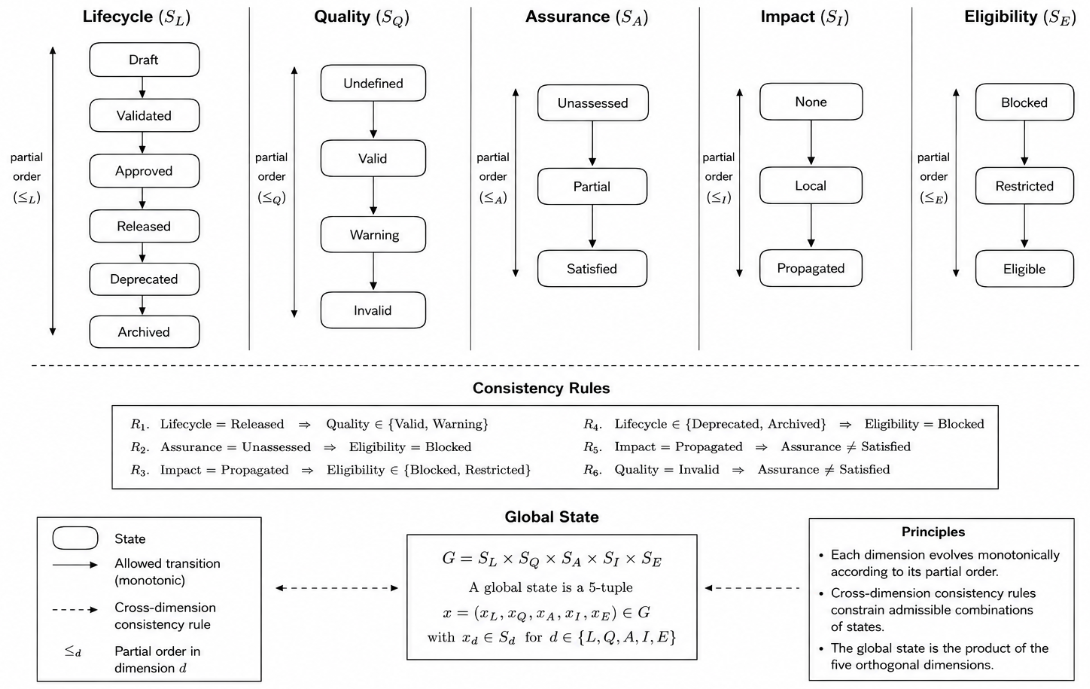
\includegraphics[width=\textwidth]{figures/othogonal_governance_state_machine.png}
	
	\caption{Orthogonal governance state machines composing the ACM governance
		semantics. Lifecycle, quality, impact, and assurance are evaluated as distinct
		state dimensions, while execution eligibility is derived through the evaluation
		function $f(L,Q,A,I)$.}
	\label{fig:governance_state_machine}
\end{figure*}

%%%%%%%%%%%%%%%%%%%%%%%%%%%%%%%%%%%%%%%%%%%%%%%%%%%%%%%%%%%%%%%%%%%%%%%%%%%%%%%%
\subsubsection{Transition Properties}

The governance state machines satisfy the following properties.

\paragraph{Property G1 (Determinism).}

For every governance event, each state machine admits exactly one successor
state.

\paragraph{Property G2 (Orthogonality).}

Each governance dimension evolves independently according to its own transition function (see Appendix section ~\ref{appendix:governance_orthogonality}).

\paragraph{Property G3 (Composability).}

The global governance state is obtained through the composition of independent semantic dimensions rather than by constructing a single global automaton.

\paragraph{Property G4 (Extensibility).}

Additional governance dimensions may be introduced without modifying the existing state machines provided that they expose well-defined evaluation functions.

These properties considerably simplify future extensions of ACM while
preserving backward compatibility of governance semantics.

The next subsection formalizes how local governance changes propagate through dependency relationships, enabling global reasoning over complete agentic configuration graphs.

Figure~\ref{fig:impact_propagation} illustrates the propagation of a local configuration change through governance dependencies. The directly modified revision receives the \textit{Local} impact state, while reachable dependent revisions receive the \textit{Propagated} state. Revisions outside the resulting impact closure remain in the \textit{None} state.

\begin{figure*}[t]
	\centering
	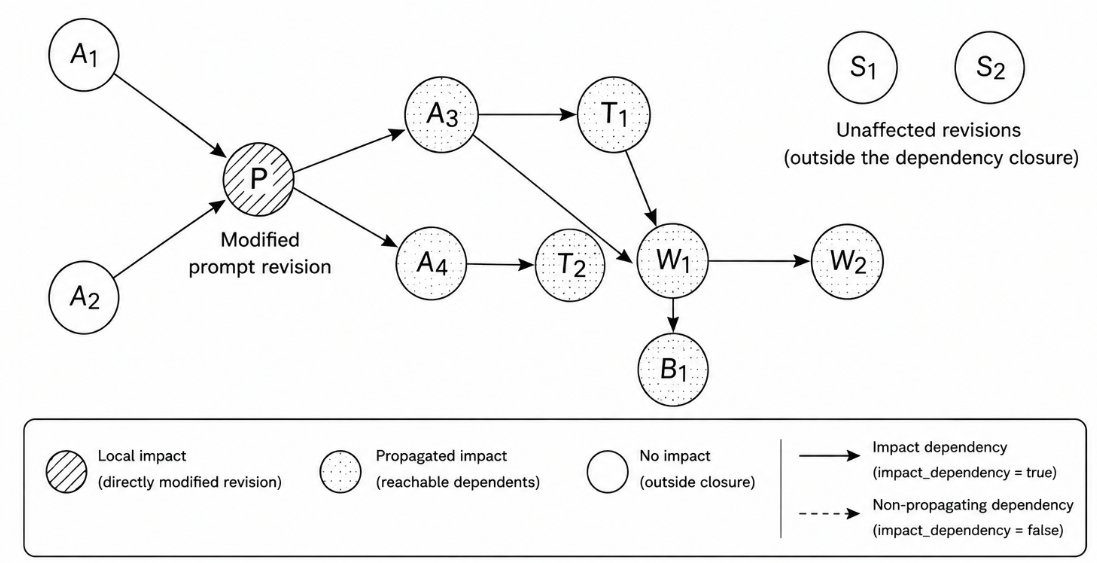
\includegraphics[width=\textwidth]{figures/Impact_propagation_revision.png}
	\caption{
		Impact propagation following the modification of prompt revision $P$.
		The directly modified revision receives a local impact state, while
		reachable dependent revisions receive a propagated impact state.
		Revisions outside the dependency closure remain unaffected.
	}
	\label{fig:impact-propagation}
\end{figure*}

%%%%%%%%%%%%%%%%%%%%%%%%%%%%%%%%%%%%%%%%%%%%%%%%%%%%%%%%%%%%%%%%%%
\subsubsection{Illustrative Example}

Assume that a workflow

\[
W
\]

contains an agent

\[
A_1
\]

whose prompt revision is modified. The prompt immediately becomes

\[
Local.
\]

The associated agent, workflow, runtime deployment, and assurance reports become:

\[
Propagated,
\]

because each depends on the modified configuration revision.

Importantly, propagation alone does not imply execution failure.

It merely indicates that governance evaluation should be recomputed before the corresponding artifacts are considered trustworthy.

Figure~\ref{fig:agent_state_before_after} illustrates the non-destructive propagation of governance state for a single agent. A change to a required prompt revision does not modify the agent revision or its intrinsic lifecycle and quality states. Instead, the propagation process recalculates the agent's impact, assurance, and eligibility states from the updated dependency context.
\begin{figure*}[t]
	\centering
	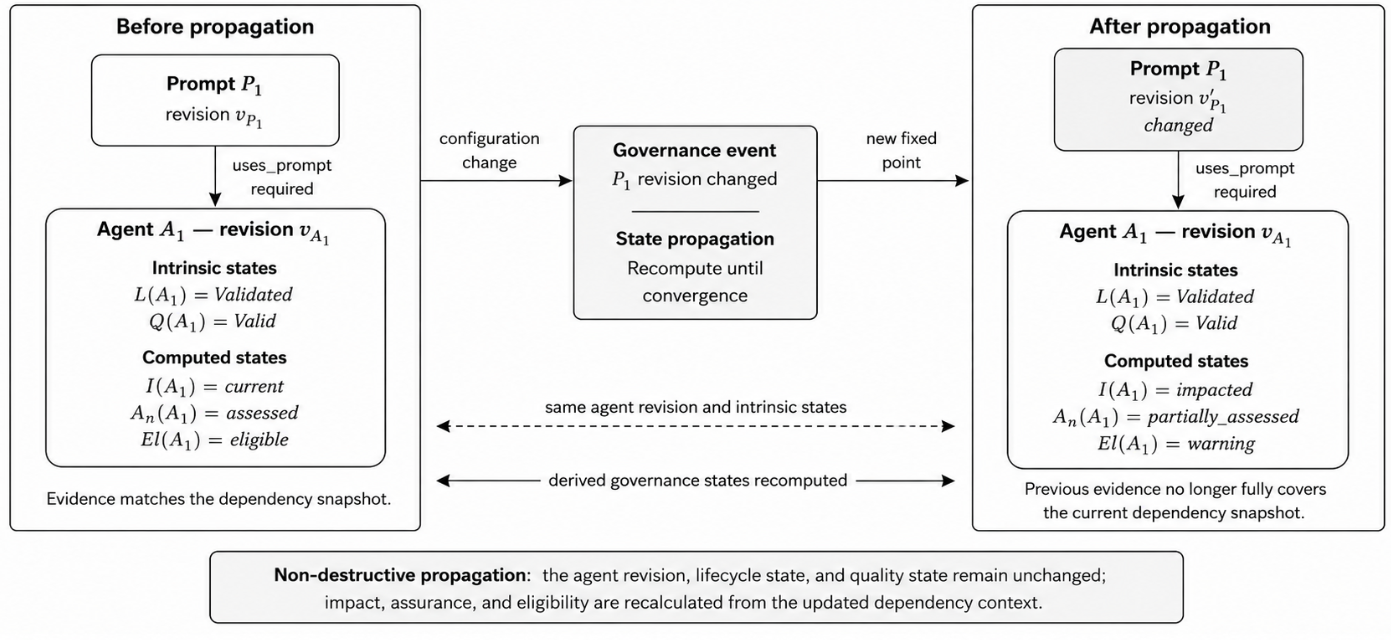
\includegraphics[width=\textwidth]{figures/non_destructive_state_propagation.png}
	
	\caption{Non-destructive governance state propagation for an agent. A change
		to a required prompt revision preserves the agent revision and its intrinsic
		lifecycle and quality states, while the derived impact, assurance, and
		eligibility states are recomputed from the updated dependency context.}
	\label{fig:agent_state_before_after}
\end{figure*}

%%%%%%%%%%%%%%%%%%%%%%%%%%%%%%%%%%%%%%%%%%%%%%%%%%%%%%%%%%%%%%%%%%%%%%%%%%%%%%%

This fixed-po nt formulation establishes the formal semantics of governance
propagation independently of any particular implementation. Whether ACM is implemented through recursive graph traversal, work-list evaluation, or incremental update algorithms, every compliant implementation is required to compute the same least fixed point, thereby guaranteeing deterministic,
reproducible, and implementation-independent governance evaluation.

Figure~\ref{fig:governance_propagation} illustrates the propagation of a prompt
deprecation through an agentic configuration. The prompt revision becomes
\texttt{deprecated}; the dependent agent becomes \texttt{impacted}; its
effective assurance is downgraded to
\texttt{partial}; and its eligibility changes from
\texttt{eligible} to
\texttt{warning}. Importantly, neither the lifecycle nor the declared quality
of the agent is modified. This example illustrates the central principle of ACM
that governance propagation affects derived governance states rather than
intrinsic configuration properties.

%%%%%%%%%%%%%%%%%%%%%%%%%%%%%%%%%%%%%%%%%%%%%%%%%%%%%%%%%%%%%%%%%%%%%%%%%%%%%%%%
% Figure to be inserted here
%
% Figure:
% Governance State Propagation
%
% (TikZ IEEE academic style)
%
%%%%%%%%%%%%%%%%%%%%%%%%%%%%%%%%%%%%%%%%%%%%%%%%%%%%%%%%%%%%%%%%%%%%%%%%%%%%%%%%
% Figure: Governance State Propagation
%%%%%%%%%%%%%%%%%%%%%%%%%%%%%%%%%%%%%%%%%%%%%%%%%%%%%%%%%%%%%%%%%%%%%%%%%%%%%%%%
\begin{figure}[t]
\centering
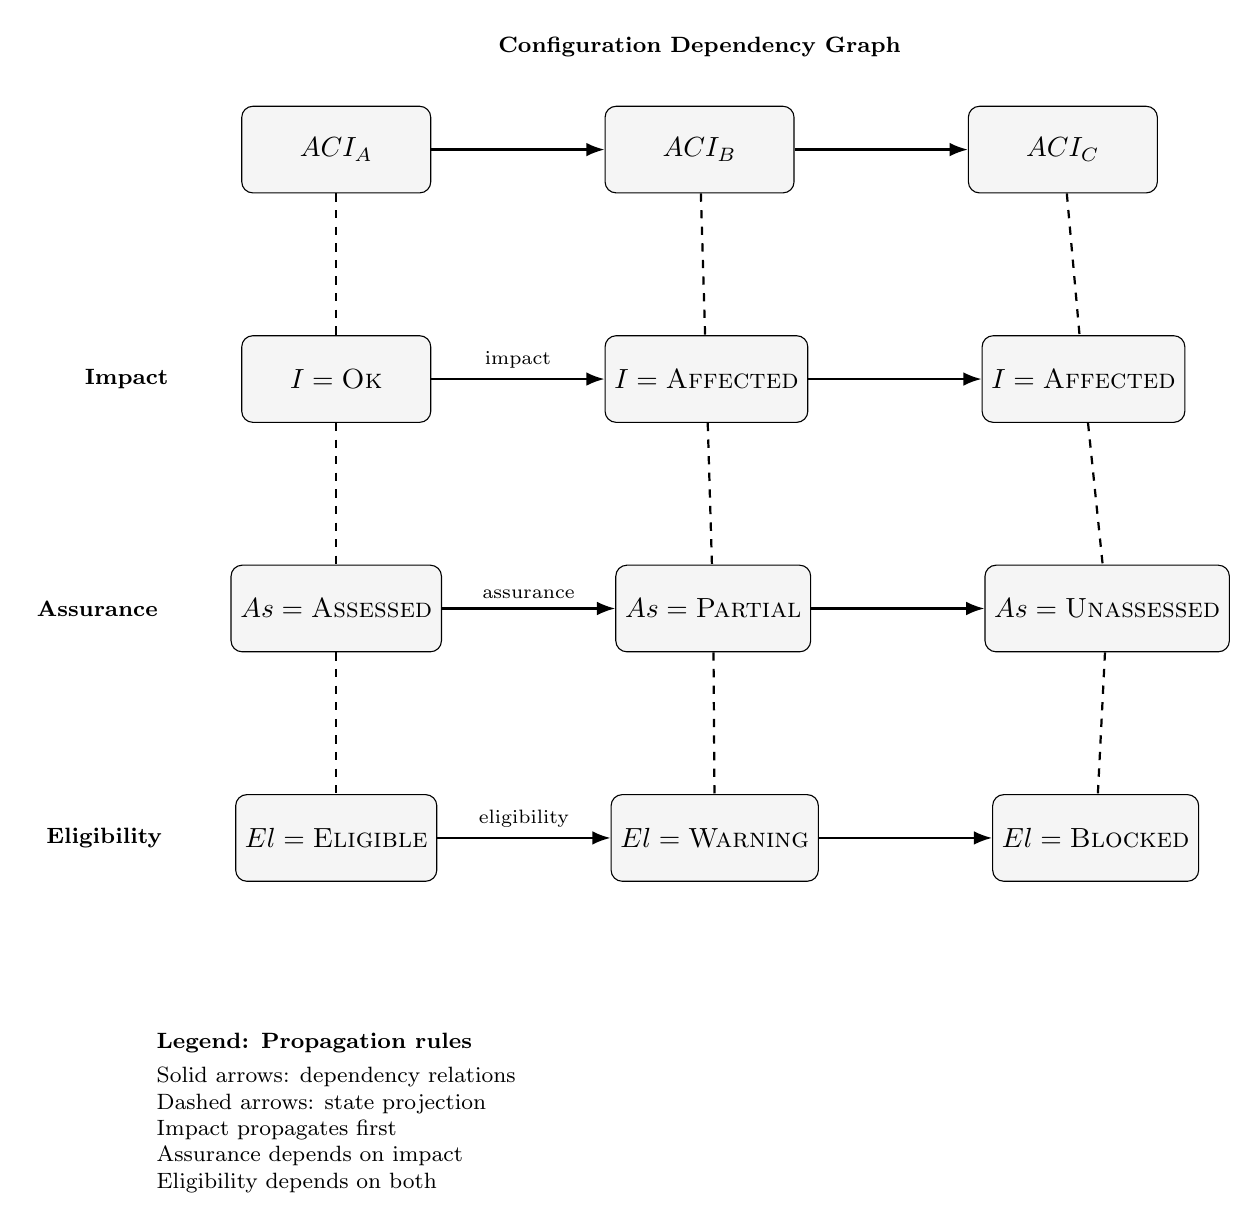
\begin{tikzpicture}[
    >=Latex,
    node distance=18mm and 22mm,
    aci/.style={
        draw,
        rounded corners,
        minimum width=24mm,
        minimum height=11mm,
        align=center,
        fill=gray!8
    },
    flow/.style={
        ->,
        thick
    },
    prop/.style={
        dashed,
        thick
    },
    annot/.style={
        font=\footnotesize,
        align=center
    }
]

%-------------------------------------------------
% Configuration graph
%-------------------------------------------------

\node[aci] (A) {$ACI_A$};
\node[aci,right=of A] (B) {$ACI_B$};
\node[aci,right=of B] (C) {$ACI_C$};

\draw[flow] (A)--(B);
\draw[flow] (B)--(C);

\node[annot,above=5mm of B]
{\textbf{Configuration Dependency Graph}};

%-------------------------------------------------
% Impact propagation
%-------------------------------------------------

\node[aci,below=18mm of A] (IA) {$I=\textsc{Ok}$};
\node[aci,right=of IA] (IB) {$I=\textsc{Affected}$};
\node[aci,right=of IB] (IC) {$I=\textsc{Affected}$};

\draw[prop] (A)--(IA);
\draw[prop] (B)--(IB);
\draw[prop] (C)--(IC);

\draw[flow] (IA)--node[above,font=\scriptsize]{impact}(IB);
\draw[flow] (IB)--node[above,font=\scriptsize]{}(IC);

\node[annot,left=8mm of IA]
{\textbf{Impact}};

%-------------------------------------------------
% Assurance propagation
%-------------------------------------------------

\node[aci,below=18mm of IA] (AA) {$As=\textsc{Assessed}$};
\node[aci,right=of AA] (AB) {$As=\textsc{Partial}$};
\node[aci,right=of AB] (AC) {$As=\textsc{Unassessed}$};

\draw[prop] (IA)--(AA);
\draw[prop] (IB)--(AB);
\draw[prop] (IC)--(AC);

\draw[flow] (AA)--node[above,font=\scriptsize]{assurance}(AB);
\draw[flow] (AB)--(AC);

\node[annot,left=8mm of AA]
{\textbf{Assurance}};

%-------------------------------------------------
% Eligibility propagation
%-------------------------------------------------

\node[aci,below=18mm of AA] (EA) {$El=\textsc{Eligible}$};
\node[aci,right=of EA] (EB) {$El=\textsc{Warning}$};
\node[aci,right=of EB] (EC) {$El=\textsc{Blocked}$};

\draw[prop] (AA)--(EA);
\draw[prop] (AB)--(EB);
\draw[prop] (AC)--(EC);

\draw[flow] (EA)--node[above,font=\scriptsize]{eligibility}(EB);
\draw[flow] (EB)--(EC);

\node[annot,left=8mm of EA]
{\textbf{Eligibility}};

%-------------------------------------------------
% Legend
%-------------------------------------------------

\node[
align=left,
below=18mm of EA,
font=\footnotesize
]
{
\textbf{Legend: Propagation rules}\\[1mm]
Solid arrows: dependency relations\\
Dashed arrows: state projection\\
Impact propagates first\\
Assurance depends on impact\\
Eligibility depends on both
};

\end{tikzpicture}

\caption{Governance state propagation across the configuration graph.
A structural dependency first propagates impact, which subsequently influences
assurance evaluation and finally execution eligibility. The three governance
dimensions remain conceptually independent while being evaluated in a
deterministic order.}
\label{fig:governance_propagation}
\end{figure}
%%%%%%%%%%%%%%%%%%%%%%%%%%%%%%%%%%%%%%%%%%%%%%%%%%%%%%%%%%%%%%%%%%%%%%%%%%%%%%%%

%%%%%%%%%%%%%%%%%%%%%%%%%%%%%%%%%%%%%%%%%%%%%%%%%%%%%%%%%%%%%%%%%%%%%%%%%%%%%%%%
\subsection{Runtime Semantics}
\label{subsec:runtime_semantics}

The governance semantics defined so far describe how configuration states evolve
within the immutable configuration graph. Runtime execution introduces an
additional dimension that cannot be represented solely by static configuration
artifacts. Agent executions create transient observations whose purpose is not
to modify the governed configuration but to record how a released baseline is
instantiated during execution.

Accordingly, ACM distinguishes the \emph{Configuration Graph}, which contains
immutable governed revisions, from the \emph{Runtime Graph}, which represents
the execution state derived from a specific released baseline. Runtime
observations never alter immutable configuration revisions. Instead, they are
associated with the corresponding governed artifacts through stable revision
identifiers and provenance relationships.

The Runtime Graph is constructed from an ordered sequence of normalized runtime
events. Each event captures an observable execution transition together with the
identifier of the corresponding governed revision. Because runtime observations
are represented independently from framework-specific execution traces, the same
governance semantics can be applied to heterogeneous execution frameworks after
semantic projection into the ACM reference model.

Rather than storing successive runtime snapshots, ACM defines the runtime state
as the result of replaying the normalized event sequence from a released
baseline. Starting from the immutable configuration represented by the baseline,
runtime events are deterministically applied in chronological order to
reconstruct the Runtime Graph corresponding to any observation point.

This separation provides two complementary benefits. First, released
configurations remain immutable throughout execution, preserving configuration
integrity and provenance. Second, runtime reconstruction becomes independent of
the execution framework, provided that equivalent normalized events are
available. Consequently, runtime analyses, governance verification, and
conformance checking operate on a canonical Runtime Graph rather than on
framework-specific execution representations.

The replay semantics are intentionally defined independently of the propagation
operator introduced in Section~\ref{sec:propagation_semantics}. Propagation
computes the stabilized governance state associated with immutable
configurations, whereas replay reconstructs the execution state generated from a
released baseline. These two mechanisms therefore address complementary
concerns: governance evaluation determines the valid configuration to be
executed, while runtime replay reconstructs how that configuration was actually
executed.

The formal definition of normalized runtime events, the replay function, the
incremental reconstruction procedure, and the associated correctness properties
are presented in Appendix ~\ref{appendix:runtime_semantics}.

\subsection{Formal Properties}
\label{sec:formal_properties}

The governance semantics defined in the previous subsections satisfy a number of
formal properties that ensure the consistency, reproducibility, and
predictability of ACM evaluations. These properties follow directly from the
state spaces, evaluation functions, propagation semantics, and runtime replay
model introduced throughout Section~5.

First, the impact propagation semantics are monotone over the finite impact
lattice defined in Appendix~A.3. Consequently, iterative propagation converges
toward the least fixed point above the initial impact valuation, while the
reference worklist algorithm computes the same stabilized result under any fair
evaluation strategy. The corresponding proofs are provided in
Appendix~A.6.

Second, runtime replay is deterministic. Given an immutable released baseline
and an identical ordered sequence of normalized runtime events, replay always
reconstructs the same Runtime Graph. This property guarantees that runtime
observations remain reproducible independently of the underlying execution
framework after semantic projection into the ACM reference model. The formal
replay model and proof of determinism are presented in Appendix~A.7.

Together, these properties establish that governance evaluation and runtime
reconstruction are reproducible and implementation-independent. For identical
governed configurations and equivalent normalized runtime observations, ACM
always produces identical governance states and identical reconstructed Runtime
Graphs. This determinism provides the foundation for reproducible governance
verification, impact analysis, runtime conformance checking, and assurance
evaluation across heterogeneous agentic frameworks.

The complete proofs, together with the complexity analysis and additional formal
results, are presented in Appendix~A.8.


























\section{Operationalization}
\label{sec:operationalization}

The purpose of this section is not to define another execution framework but to demonstrate that the proposed reference model is operationalizable without introducing framework-specific concepts into its governance semantics. The operationalization deliberately separates governance semantics from implementation details. The ACM metamodel, lifecycle semantics, and validation rules are independent of programming language, persistence technology, communication protocol, or execution framework. The Python implementation therefore serves only as one concrete realization of the reference model, demonstrating implementability rather than prescribing a specific software architecture. The experimental methodology is depicted in Figure ~\ref{fig:experimental_protocol}.

\begin{figure*}[t]
	\centering
	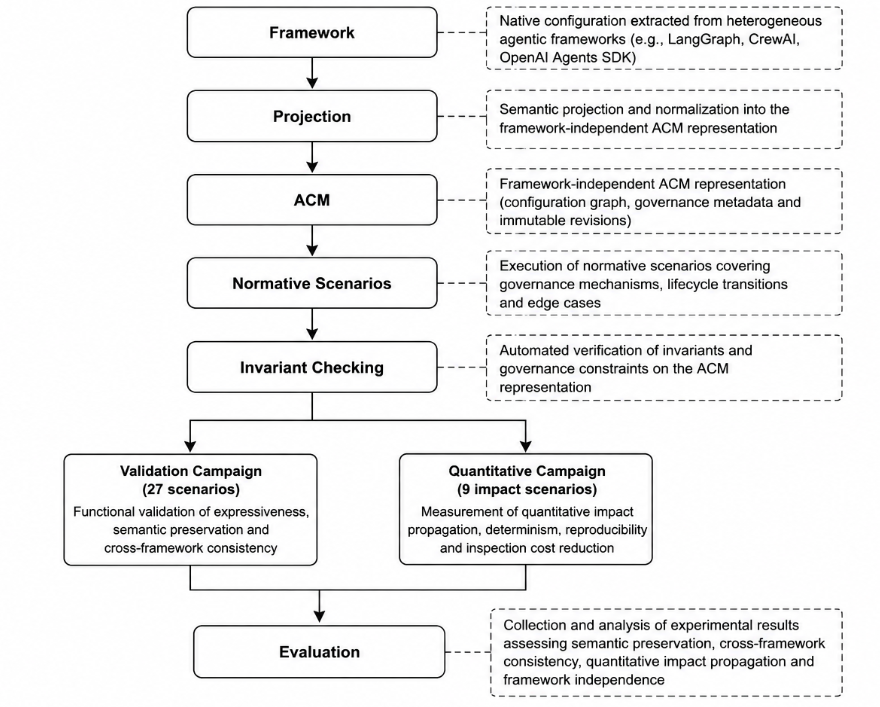
\includegraphics[width=0.5\textwidth]{figures/experimental_protocol.png}
	\caption{Overview of the experimental methodology. Native framework configurations are projected into the ACM reference model through semantic projection, validated using normative governance scenarios and automated invariant checking, and finally evaluated.}
	\label{fig:experimental_protocol}
\end{figure*}

\subsection{Reference Architecture}
\label{subsec:reference_architecture}

The ACM reference model is intentionally independent of any particular agentic framework. Its operationalization therefore adopts a layered architecture that cleanly separates framework-specific extraction from framework-independent governance. This separation preserves the conceptual independence of the reference model while allowing heterogeneous agentic systems to be represented through a common governed configuration.

In our reference architecture, framework-specific adapters extract native constructs and project them into canonical ACM revisions and relationships. All subsequent validation, propagation, assurance, eligibility, and runtime reconstruction operate exclusively on the resulting ACM representation.

The governance kernel constitutes the core of the operationalization. It implements the normative semantics introduced in Section~\ref{sec:governance_semantics}, including structural validation, lifecycle management, governance state evaluation, impact propagation, assurance evaluation, and eligibility assessment. Since these operations manipulate only canonical ACM representations, their behavior remains independent of the execution framework.

The runtime interface complements the governance kernel by exposing governed configurations together with normalized execution observations. Runtime events enrich the operational view of the system without modifying immutable configuration revisions, thereby preserving the separation between configuration governance and execution behavior.

The reference implementation should not be interpreted as a production platform or a preferred execution environment. Its purpose is to demonstrate that the ACM reference model can be operationalized through a framework-independent governance kernel while allowing multiple execution frameworks to share identical governance semantics.

The operationalization is organized into five successive stages:

\begin{enumerate}
	\item \textbf{Framework Extraction}, which retrieves governance-relevant native configuration artifacts exposed by the execution framework;
	
	\item \textbf{Semantic Projection}, which maps these native artifacts onto ACM concepts through framework-specific projection rules;
	
	\item \textbf{Canonical Normalization}, which constructs immutable ACI revisions, resolves references, assigns stable identities, computes canonical digests, and builds the governed configuration graph;
	
	\item \textbf{Governance Processing}, which applies the framework-independent governance semantics defined in Section~\ref{sec:governance_semantics};
	
	\item \textbf{Governed Representation}, which produces the normalized ACM representation used for validation, auditing, replay, impact analysis, and lifecycle management.
\end{enumerate}

This organization deliberately isolates framework-dependent concerns from governance semantics. Native frameworks remain responsible for execution, whereas ACM provides a common governance layer operating on a unified configuration representation.


\subsection{Projection Pipeline}
\label{subsec:semantic_projection_pipeline}

The reference architecture introduced in Section~\ref{subsec:reference_architecture} is realized through a semantic projection pipeline that transforms heterogeneous framework configurations into the canonical ACM representation. Rather than reproducing the internal execution model of each framework, the pipeline identifies only the constructs carrying governance significance and projects them onto the concepts defined by the ACM reference model.

The projection process consists of four successive stages:

\begin{enumerate}
	\item native structure extraction;
	\item semantic classification;
	\item canonical normalization;
	\item projection validation and coverage assessment.
\end{enumerate}

This pipeline establishes a common projection contract shared by all framework adapters. Although extraction mechanisms differ across execution frameworks, each adapter ultimately produces the same normalized ACM representation, enabling the governance kernel to operate independently of framework-specific implementation details.

The complete projection formalism is provided in Appendix~\ref{appendix:projection_formalism}.

\subsubsection{Framework-specific Instantiations}

The prototype implements this projection contract through dedicated adapters for LangGraph, CrewAI, and the OpenAI Agents SDK. These adapters differ only in the extraction phase, reflecting the distinct introspection mechanisms provided by each framework, while sharing the same normalization rules and governance semantics.

For each adapter, the evaluation reports:

\begin{itemize}
	\item the number of governance-relevant native entities;
	\item the number of completely, partially, and unsuccessfully projected entities;
	\item the number of governance-relevant native relationships;
	\item the corresponding entity, relationship, aggregate, and strict coverage scores.
\end{itemize}

The measured values are reported in Section~\ref{sec:evaluation}. They are computed from the explicit inventory of governance-relevant native constructs defined by the experimental protocol rather than inferred from the mere existence of a functioning adapter. Consequently, projection coverage evaluates the expressiveness of the ACM reference model independently of the implementation itself.


\subsection{Framework Adapters}
\label{sec:framework_adapters}

The semantic projection pipeline is realized through framework-specific adapters responsible for extracting governance-relevant configuration artifacts from native execution environments. Although the extraction mechanisms differ across frameworks, every adapter produces the same normalized ACM representation before governance processing begins. Consequently, all subsequent validation, propagation, replay, and lifecycle evaluation operate independently of the originating framework.

The current reference implementation includes adapters for LangGraph, CrewAI, and the OpenAI Agents SDK. These three frameworks intentionally represent complementary introspection regimes rather than alternative implementations of the same architecture, providing a broader validation of the projection approach.

\paragraph{LangGraph.}

LangGraph exposes an explicit execution graph whose nodes, edges, routing conditions, prompts, tools, and models can be extracted directly through framework introspection. Consequently, the projection is predominantly structural and requires only limited semantic reconstruction. Governance-relevant relationships are preserved almost directly before canonical normalization.

\paragraph{CrewAI.}

CrewAI organizes execution around crews, tasks, flows, and associated metadata. While the primary governance entities remain directly identifiable, part of the execution topology must be reconstructed from declarative configuration metadata and execution conventions. The adapter therefore combines explicit extraction with semantic reconstruction while preserving the governance semantics required by ACM.

\paragraph{OpenAI Agents SDK.}

The OpenAI Agents SDK represents agent interactions through explicit handoff relationships. Unlike workflow-oriented frameworks, delegation topology is reconstructed by introspecting agent definitions and their declared handoffs rather than by traversing an explicit workflow graph. This demonstrates that ACM does not depend on a single representation of execution topology and can normalize heterogeneous delegation mechanisms into the same governance model.

Table~\ref{tab:framework_projection_summary} summarizes the principal characteristics of the three adapters.

\begin{table}[t]
	\centering
	\caption{Comparison of framework-specific projection mechanisms.}
	\label{tab:framework_projection_summary}
	\small
	\begin{tabular}{p{3.0cm}p{2.6cm}p{2.8cm}p{2.8cm}}
		\toprule
		\textbf{Characteristic} &
		\textbf{LangGraph} &
		\textbf{CrewAI} &
		\textbf{OpenAI Agents SDK} \\
		\midrule
		Primary topology &
		Explicit execution graph &
		Flow and task structure &
		Agent handoffs \\
		Governance entities &
		Direct extraction &
		Direct extraction &
		Direct extraction \\
		Relationship recovery &
		Structural &
		Hybrid reconstruction &
		Delegation introspection \\
		Semantic normalization &
		Direct &
		Hybrid &
		Direct \\
		Governance kernel &
		Common ACM representation &
		Common ACM representation &
		Common ACM representation \\
		\bottomrule
	\end{tabular}
\end{table}

Together, these adapters cover three complementary introspection regimes while preserving a common governance representation. The objective of the adapters is therefore not to reproduce framework-specific execution semantics but to expose a normalized configuration model suitable for framework-independent governance.
These three adapters demonstrate that the operationalization is not tied to a particular representation of agentic systems. Instead, heterogeneous native abstractions are normalized into a common governance representation that is subsequently processed by the same framework-independent governance algorithms.

\subsection{Governance Algorithms}
\label{sec:governance_algorithms}

The reference implementation realizes the ACM governance semantics through four framework-independent algorithms operating exclusively on normalized ACM representations. Their purpose is not to redefine the formal semantics introduced in Section~\ref{sec:governance_semantics}, but to provide a deterministic operational realization suitable for heterogeneous execution frameworks. Figure~\ref{fig:governance_processing_pipeline} summarizes this workflow.

\begin{figure}[ht]
\centering
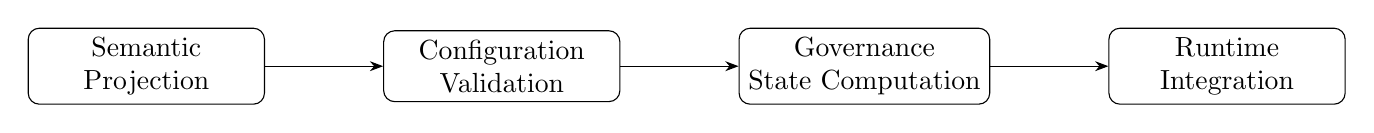
\begin{tikzpicture}[
node distance=1.5cm,
every node/.style={
draw,
rounded corners,
align=center,
minimum width=3cm,
minimum height=0.8cm
},
>=Stealth
]

\node (projection) {Semantic\\Projection};
\node (validation) [right=of projection] {Configuration\\Validation};
\node (states) [right=of validation] {Governance\\State Computation};
\node (runtime) [right=of states] {Runtime\\Integration};

\draw[->] (projection) -- (validation);
\draw[->] (validation) -- (states);
\draw[->] (states) -- (runtime);

\end{tikzpicture}

\caption{Governance processing pipeline implemented by the reference operationalization.}
\label{fig:governance_processing_pipeline}
\end{figure}

\paragraph{Algorithm 1 --- Semantic Projection}

The projection algorithm transforms native framework artifacts into immutable
ACM revisions and relationships while preserving governance-relevant semantics.

\begin{algorithm}[t]
	\caption{Semantic Projection}
	\begin{enumerate}
		\item \textbf{Input:} native framework configuration.
		\item Extract governance-relevant native entities.
		\item Identify relationships and associated metadata.
		\item Map native constructs to ACM concepts.
		\item Normalize identities and references.
		\item Compute canonical digests.
		\item Construct immutable ACM revisions and relationships.
		\item \textbf{Output:} normalized ACM Configuration Graph.
	\end{enumerate}
\end{algorithm}

\paragraph{Algorithm 2 --- Configuration Validation}

Structural validation verifies the integrity of the normalized configuration
before governance evaluation.

\begin{algorithm}[t]
	\caption{Configuration Validation}
	\begin{enumerate}
		\item \textbf{Input:} normalized ACM Configuration Graph.
		\item Verify structural consistency.
		\item Resolve cross-references.
		\item Validate lifecycle constraints.
		\item Check applicable governance invariants.
		\item Record validation results.
		\item \textbf{Output:} validated Configuration Graph.
	\end{enumerate}
\end{algorithm}

\paragraph{Algorithm 3 --- Governance Evaluation}

Governance evaluation combines local state computation with deterministic
impact propagation until stabilization. The algorithm operationalizes the
semantics defined in Section~\ref{sec:governance_semantics} without redefining
their formal specification.

\begin{algorithm}[t]
	\caption{Governance Evaluation}
	\begin{enumerate}
		\item \textbf{Input:} validated Configuration Graph.
		\item Compute local governance states.
		\item Initialize the impact state from the detected configuration change.
		\item Initialize the propagation worklist.
		\item While the worklist is not empty:
		\begin{enumerate}
			\item select one pending ACI;
			\item propagate impact through applicable relationships;
			\item update impacted dependents when their state increases;
			\item enqueue dependents whose state has changed.
		\end{enumerate}
		\item Evaluate eligibility from the stabilized local and impact states.
		\item \textbf{Output:} governed Configuration Graph.
	\end{enumerate}
\end{algorithm}

\paragraph{Algorithm 4 --- Runtime Integration}

Runtime observations are normalized into governance events that incrementally
reconstruct the Runtime Graph without modifying immutable configuration
revisions.

\begin{algorithm}[t]
	\caption{Runtime Integration}
	\begin{enumerate}
		\item \textbf{Input:} normalized runtime event stream.
		\item For each event:
		\begin{enumerate}
			\item validate event consistency;
			\item append the event to the ordered event log;
			\item apply the event to the current Runtime Graph.
		\end{enumerate}
		\item Replay the ordered event log when reconstruction is requested.
		\item \textbf{Output:} updated or reconstructed Runtime Graph.
	\end{enumerate}
\end{algorithm}

Table~\ref{tab:algorithm_complexity} summarizes the asymptotic complexity of the principal operational algorithms.

\begin{table}[t]
	\centering
	\caption{Asymptotic complexity of the reference algorithms.}
	\label{tab:algorithm_complexity}
	\small
	\begin{tabular}{lc}
		\toprule
		\textbf{Algorithm} & \textbf{Complexity} \\
		\midrule
		Semantic Projection & $O(|V|+|E|)$ \\
		Configuration Validation & $O(|V|+|E|)$ \\
		Governance Evaluation & $O(k(|V|+|E|))$ \\
		Runtime Replay & $O(|R|)$ \\
		\bottomrule
	\end{tabular}
\end{table}

The reference implementation emphasizes deterministic behavior and semantic reproducibility rather than execution performance. The detailed implementation architecture is presented in the following subsection, while the formal properties of the propagation algorithm are established in Section~\ref{sec:governance_semantics} and its appendix.

\subsection{Reference Implementation}
\label{sec:reference_implementation}

The reference implementation provides an executable operationalization of the ACM reference model. It is intended to demonstrate the feasibility and reproducibility of the proposed governance semantics rather than to serve as a production-ready orchestration platform.

The prototype is implemented in Python~3.11--3.13 using Pydantic~v2 to enforce strict data contracts, immutable configuration revisions, and schema validation. Its modular organization separates framework-specific extraction from framework-independent governance, allowing new execution frameworks to be integrated by implementing only an additional projection adapter while leaving the governance kernel unchanged.

The implementation is organized into five principal modules:

\begin{itemize}
	\item \textbf{Core models}, providing immutable ACI revisions, configuration graphs, release baselines, governance descriptors, runtime objects, and canonical serialization;
	\item \textbf{Governance engine}, implementing validation, governance state evaluation, impact propagation, lifecycle management, and runtime reconstruction;
	\item \textbf{Framework adapters}, responsible for semantic projection from native framework representations into canonical ACM objects;
	\item \textbf{Scenario harness}, providing reproducible experimental scenarios, semantic-preservation analyses, quantitative impact evaluation, and report generation;
	\item \textbf{Verification suite}, comprising unit tests, property-based tests, and regression tests validating both the governance semantics and framework projections.
\end{itemize}

Canonical serialization, immutable revisions, and deterministic governance evaluation ensure that identical configurations always produce identical governed representations. This reproducibility is further reinforced by normalized runtime events, replayable execution histories, and deterministic impact propagation, allowing governance analyses to be reproduced independently of the underlying execution framework.

The modular organization also facilitates extensibility. Supporting an additional framework requires only the implementation of a new semantic projection adapter satisfying the common projection contract introduced in Section~\ref{subsec:semantic_projection_pipeline}; the governance kernel, runtime semantics, and evaluation algorithms remain unchanged (see Figure ~\ref{fig:operationalization_acm}).

\begin{figure*}[t]
	\centering
	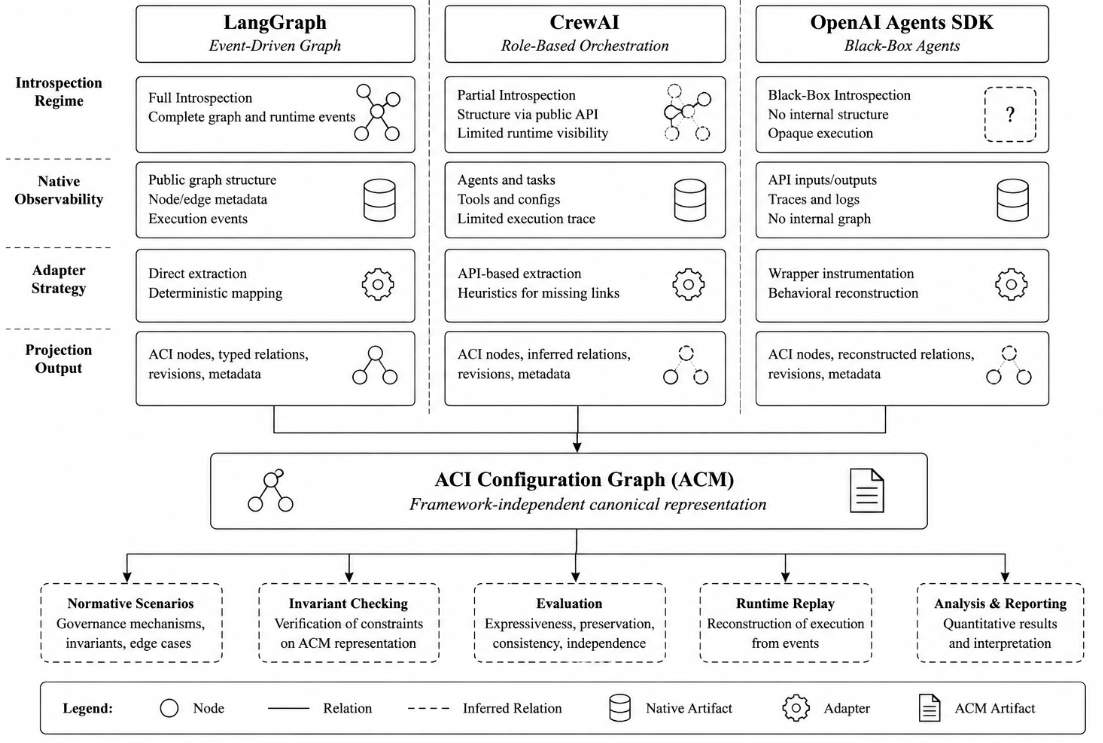
\includegraphics[width=\textwidth]{figures/operationalization_acm.png}
	\caption{Operationalization of the ACM reference model through semantic projection. Native framework configurations are projected into a common framework-independent governance representation, while a reference implementation demonstrates validation, runtime replay and conformance, and impact analysis based on the ACM governance semantics.}
	\label{fig:operationalization_acm}
\end{figure*}
\paragraph{Algorithm Overview}
Table ~\ref{tab:governance_algorithms} summarizes the governance of the implemented algorithms by the ACM reference prototype.

\begin{table}[t]
	\centering
	\caption{Core governance algorithms implemented by the ACM reference prototype.}
	\label{tab:governance_algorithms}
	\small
	\renewcommand{\arraystretch}{1.15}
	\begin{tabularx}{\columnwidth}{>{\raggedright\arraybackslash}p{2.8cm}XX>{\raggedright\arraybackslash}p{2.6cm}}
		\toprule
		\textbf{Algorithm} &
		\textbf{Input} &
		\textbf{Output} &
		\textbf{Main Purpose} \\
		\midrule
		
		Semantic Projection &
		Native framework configuration &
		Canonical ACM configuration graph &
		Semantic normalization \\
		
		Structural Validation &
		ACM configuration graph &
		Validated ACM configuration graph &
		Structural integrity verification \\
		
		Governance Evaluation &
		Validated ACM configuration graph &
		Governance-annotated ACM graph &
		Governance state computation \\
		
		Runtime Integration &
		Normalized runtime events &
		ACM runtime graph &
		Replay and execution reconstruction \\
		
		\bottomrule
	\end{tabularx}
\end{table}

\paragraph{Experimental Instrumentation.}

The reference implementation additionally includes an experimental instrumentation layer used exclusively for the evaluation reported in Section~\ref{sec:evaluation}. This layer collects projection inventories, semantic-preservation outcomes, normalized impact-propagation results, reproducibility metadata, and comparison data used by the experimental protocol. It remains separated from the governance kernel and does not participate in the computation of normative ACM states. This separation ensures that the evaluation infrastructure observes and measures the operationalization without altering the semantics being evaluated.


\section{Evaluation}
\label{sec:evaluation}

This section evaluates the ACM reference model with respect to the research questions introduced in Section~\ref{sec:introduction}. The objective is to assess whether the proposed reference model preserves governance semantics across heterogeneous agentic frameworks, supports deterministic governance evaluation, and provides a framework-independent foundation for agentic configuration management. The evaluation combines two complementary experimental campaigns. The first validates the expressiveness of the reference model, the preservation of its governance semantics, and its cross-framework applicability through twenty-seven governance scenarios executed on LangGraph, CrewAI, and the OpenAI Agents SDK. The second complements this validation with a dedicated quantitative evaluation of impact propagation across nine additional cases. Together, both campaigns provide evidence for the four research questions addressed in this work.

\subsection{Research Questions}
\label{sec:research_questions}

The evaluation addresses the following research questions.

\begin{itemize}
	
	\item \textbf{RQ1 -- Reference Model Expressiveness.}
	Can heterogeneous agentic frameworks be represented using the ACM reference model while preserving governance-relevant configuration concepts?
	
	\item \textbf{RQ2 -- Governance Semantics.}
	Does the operationalization faithfully realize the governance semantics defined in Section~\ref{sec:governance_semantics}, including lifecycle management, governance evaluation, impact propagation, release governance, and runtime reconstruction?
	
	\item \textbf{RQ3 -- Framework Independence.}
	Can equivalent governed representations be obtained from heterogeneous execution frameworks through semantic projection into a common ACM representation?
	
	\item \textbf{RQ4 -- Quantitative Impact Analysis.}
	Can the governance kernel produce deterministic and reproducible impact analyses across heterogeneous frameworks while reducing the set of configuration elements requiring manual inspection?
	
\end{itemize}

The first three research questions evaluate the reference model itself, whereas the fourth assesses the operational behavior of the governance kernel through a dedicated quantitative impact analysis.
The following sections describe the experimental methodology adopted to answer these research questions and present the empirical evidence collected using the reference implementation.


\subsection{Experimental Design}
\label{sec:experimental_protocol}

The evaluation follows two complementary experimental campaigns designed to assess distinct properties of the ACM reference model.

\subsubsection{Campaign A -- Reference Model Validation} The first campaign evaluates the expressiveness of the reference model, the preservation of its governance semantics, and its applicability across heterogeneous agentic frameworks. It consists of twenty-seven controlled governance scenarios covering the principal concepts introduced throughout the reference model, including immutable revisions, lifecycle evolution, governance states, dependency propagation, release baselines, runtime governance, dynamic agents, and semantic projection. The complete scenario suite is executed independently on LangGraph, CrewAI, and the OpenAI Agents SDK through their respective projection adapters. Each native configuration is projected into the canonical ACM representation before governance processing, while the same framework-independent governance kernel is used for all three frameworks. This design makes it possible to distinguish framework-specific extraction from the semantics evaluated by the ACM core. Each scenario specifies an initial governed configuration, the sequence of configuration or runtime events applied to the system, and the expected governance outcomes. The resulting governed representations are compared against the expected semantic properties defined by the reference model. Collectively, the twenty-seven scenarios provide evidence for RQ1 and RQ2, while their execution across the three frameworks directly supports RQ3 by testing whether heterogeneous native representations converge toward equivalent governed ACM representations (Table ~\ref{tab:qualitative_validation} summarizes the main results associated to the Research Questions). 

\begin{table}[t]
	\caption{Coverage of the qualitative validation campaign. The 27 governance scenarios collectively exercise the main semantic capabilities of the ACM reference model across the supported execution frameworks.}
	\label{tab:qualitative_validation}
	\centering
	\footnotesize
	\begin{tabular}{p{3.2cm}p{4.5cm}p{1.8cm}c}
		\toprule
		\textbf{Validation aspect} &
		\textbf{Representative capabilities} &
		\textbf{Research question(s)} &
		\textbf{Result} \\
		\midrule
		
		Configuration model
		&
		ACI revisions, configuration relationships, release baselines, governance descriptors
		&
		RQ1
		&
		Passed
		\\
		
		Governance semantics
		&
		Lifecycle transitions, quality assessment, assurance evaluation, impact propagation, eligibility computation
		&
		RQ2
		&
		Passed
		\\
		
		Framework-independent projection
		&
		Semantic projection from LangGraph, CrewAI, and OpenAI Agents SDK into a common ACM representation
		&
		RQ3
		&
		Passed
		\\
		
		Runtime governance
		&
		Runtime event representation, execution replay, provenance reconstruction, deterministic state reconstruction
		&
		RQ2, RQ3
		&
		Passed
		\\
		
		Cross-framework consistency
		&
		Equivalent governance outcomes obtained from semantically equivalent native implementations
		&
		RQ3
		&
		Passed
		\\
		
		\bottomrule
	\end{tabular}
\end{table}

\subsubsection{Campaign B -- Quantitative Impact Evaluation} The second campaign focuses specifically on the quantitative behavior of impact propagation. Three representative configuration changes are evaluated for each of the same three frameworks, corresponding to local, intermediate, and global propagation scopes, resulting in nine additional experimental cases. Each case is executed five consecutive times to assess deterministic behavior and reproducibility. The same framework-independent fixed-point propagation engine is used throughout the evaluation. For every experimental case, the evaluation records the governed impact set, impact size, impact ratio, comparison with pre-specified reference impact sets established independently from the propagation engine, fixed-point convergence characteristics, reproducibility indicators, and estimated inspection reduction. This second campaign provides dedicated quantitative evidence for RQ4 while complementing the broader semantic validation performed in Campaign A  (see Figure ~\ref{fig:evaluation_methodology} that summarizes the methodology). 

\begin{figure}[ht]
	\centering
	
	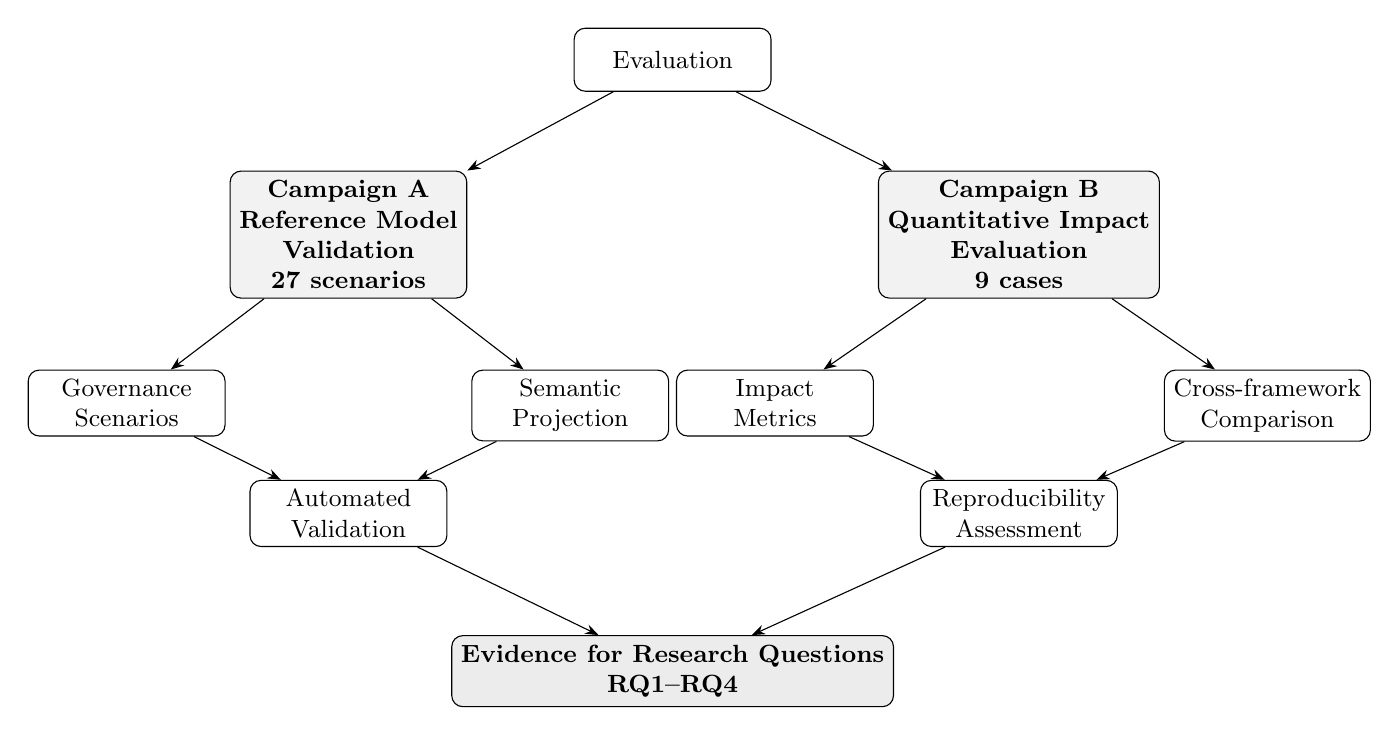
\begin{tikzpicture}[
		node distance=0.8cm and 1cm,
		>=Stealth,
		process/.style={
			draw,
			rounded corners,
			align=center,
			minimum width=2.5cm,
			minimum height=0.8cm,
			font=\small
		},
		campaign/.style={
			draw,
			rounded corners,
			fill=gray!10,
			align=center,
			minimum width=3cm,
			minimum height=0.8cm,
			font=\small\bfseries
		},
		rq/.style={
			draw,
			rounded corners,
			fill=gray!15,
			align=center,
			minimum width=3.8cm,
			minimum height=0.7cm,
			font=\small\bfseries
		}
		]
		
		% Top
		\node[process] (eval) {Evaluation};
		
		% Campaigns
		\node[campaign, below left=1cm and 1.35cm of eval] (campA)
		{Campaign A\\Reference Model\\Validation\\27 scenarios};
		
		\node[campaign, below right=1cm and 1.35cm of eval] (campB)
		{Campaign B\\Quantitative Impact\\Evaluation\\9 cases};
		
		% Campaign A activities
		\node[process, below left=0.9cm and 0.05cm of campA] (scenarios)
		{Governance\\Scenarios};
		
		\node[process, below right=0.9cm and 0.05cm of campA] (projection)
		{Semantic\\Projection};
		
		% Campaign B activities
		\node[process, below left=0.9cm and 0.05cm of campB] (impact)
		{Impact\\Metrics};
		
		\node[process, below right=0.9cm and 0.05cm of campB] (comparison)
		{Cross-framework\\Comparison};
		
		% Intermediate evidence nodes
		\node[process, below=2.3cm of campA] (validation)
		{Automated\\Validation};
		
		\node[process, below=2.3cm of campB] (repro)
		{Reproducibility\\Assessment};
		
		% Bottom
		\node[rq, below=1.5cm of eval, yshift=-5.4cm] (rqs)
		{Evidence for Research Questions\\RQ1--RQ4};
		
		% Connections
		\draw[->] (eval) -- (campA);
		\draw[->] (eval) -- (campB);
		
		\draw[->] (campA) -- (scenarios);
		\draw[->] (campA) -- (projection);
		\draw[->] (scenarios) -- (validation);
		\draw[->] (projection) -- (validation);
		
		\draw[->] (campB) -- (impact);
		\draw[->] (campB) -- (comparison);
		\draw[->] (impact) -- (repro);
		\draw[->] (comparison) -- (repro);
		
		\draw[->] (validation) -- (rqs);
		\draw[->] (repro) -- (rqs);
		
	\end{tikzpicture}
	
	\caption{Experimental methodology adopted to evaluate the ACM reference model. Campaign A validates the reference model through 27 governance scenarios and semantic projection, whereas Campaign B evaluates quantitative impact propagation across nine cross-framework cases. Together, both campaigns provide complementary evidence for RQ1--RQ4.}
	
	\label{fig:evaluation_methodology}
	
\end{figure}

Table~\ref{tab:rq_validation} summarizes how the two complementary experimental campaigns collectively address the four research questions investigated in this work.
\begin{table}[t]
	\caption{Relationship between the research questions, the experimental evidence, and the corresponding validation results.}
	\label{tab:rq_validation}
	\centering
	\footnotesize
	\begin{tabular}{p{1.0cm}p{4.0cm}p{4.2cm}p{3.0cm}}
		\toprule
		\textbf{RQ} &
		\textbf{Research objective} &
		\textbf{Experimental evidence} &
		\textbf{Main result} \\
		\midrule
		
		RQ1 &
		Can ACM represent heterogeneous agentic configurations using a unified governance model?
		&
		Qualitative validation campaign (27 governance scenarios) covering the complete ACM metamodel.
		&
		All evaluated configuration concepts were successfully represented using the ACM reference model.
		\\
		
		RQ2 &
		Does ACM preserve governance semantics independently of the native execution framework?
		&
		Cross-framework execution of governance scenarios, including lifecycle, quality, assurance, impact propagation, runtime reconstruction, and baseline evaluation.
		&
		Equivalent governance semantics were obtained after semantic projection across all evaluated frameworks.
		\\
		
		RQ3 &
		Can ACM provide a framework-independent governance layer?
		&
		Semantic projection of LangGraph, CrewAI, and OpenAI Agents SDK into a common ACM representation.
		&
		Framework-specific implementations produced equivalent governed configuration graphs and governance outcomes.
		\\
		
		RQ4 &
		Can ACM quantitatively characterize configuration impact while remaining deterministic and reproducible?
		&
		Quantitative impact evaluation on nine representative change scenarios executed across three frameworks with repeated executions.
		&
		Deterministic impact propagation, identical governed impact sets across frameworks, and reproducible quantitative metrics were obtained for all evaluated scenarios.
		\\
		
		\bottomrule
	\end{tabular}
\end{table}

\subsection{Validation of the Reference Model}
\label{sec:reference_model_validation}

Campaign~A evaluates the ACM reference model through a suite of twenty-seven controlled governance scenarios executed independently on LangGraph, CrewAI, and the OpenAI Agents SDK. The objective is not to benchmark execution performance, but to verify that heterogeneous native configurations can be projected into equivalent governed ACM representations while preserving the governance semantics defined in Section~\ref{sec:governance_semantics}.

The scenario suite was designed to exercise the principal concepts introduced throughout the reference model. Collectively, the scenarios cover immutable ACI revisions, lifecycle evolution, governance states, structural relationships, semantic projection, release baselines, runtime governance, dependency propagation, and dynamic agent evolution. Rather than validating isolated software components, each scenario evaluates the interaction between several governance mechanisms under representative configuration changes.

For every scenario, equivalent native configurations were implemented for the three supported frameworks. After semantic projection, the resulting ACM representations were processed by the same framework-independent governance kernel. The observed governed representations were then compared against the expected governance outcomes defined by the experimental specification. This protocol evaluates both the correctness of semantic projection and the preservation of governance semantics independently of the originating execution framework.

Table~\ref{tab:scenario_categories} summarizes the categories covered by the experimental campaign.

\begin{table}[t]
	\centering
	\caption{Coverage of the reference model validation scenarios.}
	\label{tab:scenario_categories}
	\small
	\begin{tabular}{p{3.2cm}p{3.8cm}}
		\toprule
		\textbf{Category} & \textbf{Representative governance aspects} \\
		\midrule
		Revision management &
		Immutable revisions, promotion, lifecycle evolution \\
		Dependency management &
		Structural relationships and impact dependencies \\
		Governance evaluation &
		Eligibility assessment, governance states, policy evaluation \\
		Release governance &
		Baseline composition, revision consistency, release evolution \\
		Runtime governance &
		Execution events and runtime reconstruction \\
		Dynamic evolution &
		Dynamic agents and evolving configurations \\
		Semantic projection &
		Cross-framework normalization and representation consistency \\
		\bottomrule
	\end{tabular}
\end{table}

Across the complete campaign, the twenty-seven scenarios produced governed representations consistent with the expected semantic properties on all three execution frameworks. No framework-specific governance behavior was introduced after semantic projection, indicating that governance evaluation depends exclusively on the normalized ACM representation rather than on the native execution model.

These observations provide complementary evidence for the first three research questions. The breadth of the scenario suite supports the expressiveness of the reference model (RQ1), the agreement between the operationalization and the formal governance semantics (RQ2), and the ability to obtain equivalent governed representations from heterogeneous execution frameworks through semantic projection (RQ3). The quantitative characteristics of impact propagation are evaluated separately in Campaign~B.

\subsection{Cross-framework Semantic Projection}
\label{sec:cross_framework_projection}

The objective of this evaluation is to determine whether heterogeneous execution frameworks can be projected into equivalent governed ACM representations while preserving the governance-relevant information required by the reference model. This experiment addresses RQ3 by evaluating the semantic projection implemented for LangGraph, CrewAI, and the OpenAI Agents SDK.

Although the three frameworks support comparable agentic applications, they expose substantially different introspection mechanisms. LangGraph provides an explicit workflow graph whose nodes and structural relationships can be reconstructed directly through framework introspection. CrewAI separates orchestration into Crew and Flow abstractions, requiring part of the execution topology to be reconstructed from adapter metadata because the complete graph is not statically introspectable. In contrast, the OpenAI Agents SDK exposes delegation explicitly through agent handoffs, allowing the delegation graph to be reconstructed directly while agent-level references remain normalized through adapter metadata. These three frameworks therefore represent complementary introspection regimes while sharing the same ACM governance model after semantic projection.

To evaluate information preservation, representative native workflows were extracted independently from each framework and compared with manually established golden representations over the normative ACM perimeter. Each extracted property was classified as \emph{preserved}, \emph{approximated}, or \emph{unsupported}, allowing the evaluation to distinguish exact reconstruction from intentional semantic abstraction.

Table~\ref{tab:projection_results} summarizes the principal information-preservation metrics obtained across the three frameworks.

\begin{table*}[t]
	\centering
	\caption{Summary of information preservation after semantic projection.}
	\label{tab:projection_results}
	\small
	\begin{tabular}{lccc}
		\toprule
		\textbf{Metric}
		&
		\textbf{LangGraph}
		&
		\textbf{CrewAI}
		&
		\textbf{OpenAI Agents SDK}
		\\
		\midrule
		Node coverage & 100\% & 100\% & 100\% \\
		Relationship coverage & 100\% & 100\% & 100\% \\
		Branch coverage & 100\% & 100\% & 100\% \\
		Entry point preserved & Yes & Yes & Yes \\
		Terminal nodes preserved & Yes & Yes & Yes \\
		Agent--prompt references & 100\% & 100\% & 100\% \\
		Agent--tool references & 100\% & 100\% & 100\% \\
		Stable extraction digest & Yes & Yes & Yes \\
		Normative properties preserved & 10 & 9--10 & 10 \\
		Approximated properties & 1 & 1 & 1 \\
		Unsupported properties & 0 & 0--1 & 0 \\
		\bottomrule
	\end{tabular}
\end{table*}

While the overall preservation results are comparable, the extraction process differs significantly between frameworks. LangGraph exposes its execution topology directly through the native workflow graph. CrewAI illustrates the limits of static introspection: workflow nodes are extracted from the Flow definition, whereas part of the orchestration topology must be supplied through adapter metadata because it is resolved dynamically at execution time. Conversely, the OpenAI Agents SDK exposes the delegation topology explicitly through handoff relationships, allowing the corresponding graph to be reconstructed entirely by introspection without unresolved structural elements.

These observations demonstrate that ACM does not depend on a single execution abstraction or introspection mechanism. Instead, semantic projection normalizes heterogeneous native representations into a common governed configuration while explicitly documenting the origin of extracted information. Consequently, differences in framework introspectability remain confined to the extraction stage and do not affect the governance semantics subsequently evaluated by the framework-independent governance kernel.

Collectively, these results support RQ3 by showing that heterogeneous native representations converge toward equivalent ACM governance models despite relying on fundamentally different extraction mechanisms. The quantitative behavior of the resulting governance semantics is evaluated separately in Campaign~B.

\subsection{Research Questions}
\label{sec:research_questions}

The evaluation addresses the following research questions.

\begin{itemize}
	
	\item \textbf{RQ1 -- Reference Model Expressiveness.}
	Can heterogeneous agentic frameworks be represented using the ACM reference model while preserving governance-relevant configuration concepts?
	
	\item \textbf{RQ2 -- Governance Semantics.}
	Does the operationalization faithfully realize the governance semantics defined in Section~\ref{sec:governance_semantics}, including lifecycle management, governance evaluation, impact propagation, release governance, and runtime reconstruction?
	
	\item \textbf{RQ3 -- Framework Independence.}
	Can equivalent governed representations be obtained from heterogeneous execution frameworks through semantic projection into a common ACM representation?
	
	\item \textbf{RQ4 -- Quantitative Impact Analysis.}
	Can the governance kernel produce deterministic and reproducible impact analyses across heterogeneous frameworks while reducing the set of configuration elements requiring manual inspection?
	
\end{itemize}

The first three research questions evaluate the reference model itself, whereas the fourth assesses the operational behavior of the governance kernel through a dedicated quantitative impact analysis.
The following sections describe the experimental methodology adopted to answer these research questions and present the empirical evidence collected using the reference implementation.

Figure ~\ref{fig:introspection_framework} summarizes the overall experimental design.
\begin{figure*}[t]
	\centering
	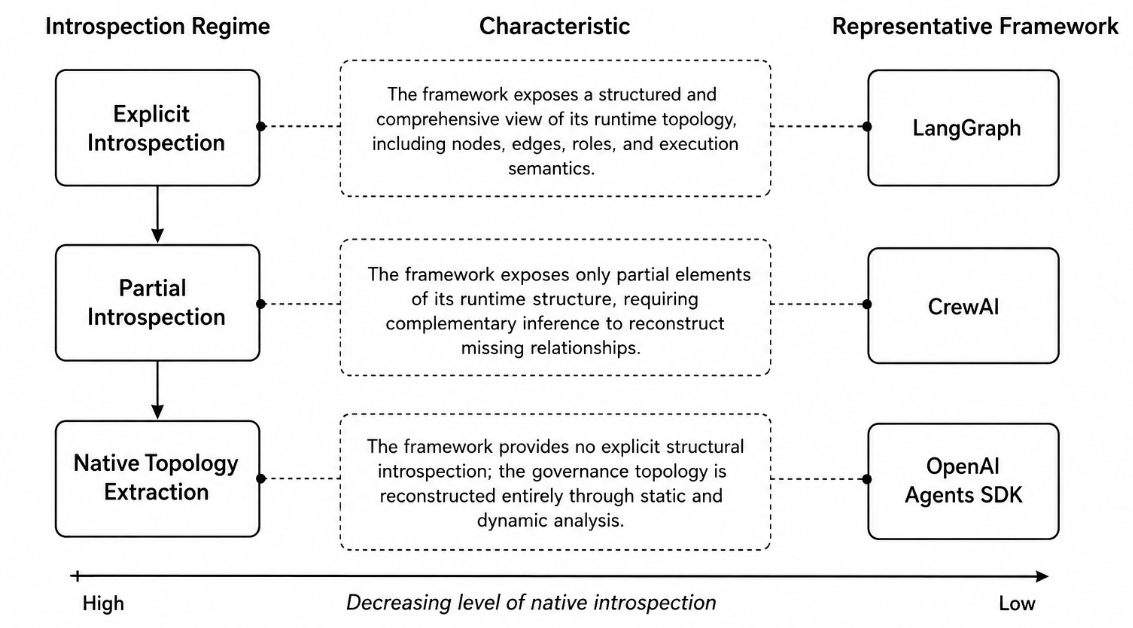
\includegraphics[width=0.7\textwidth]{figures/introspection_framework.png}
	\caption{The three introspection regimes of the evaluated frameworks. From explicit runtime introspection to native topological extraction, ACM relies on semantic projection to reconstruct a unified governance topology across heterogeneous execution platforms}
	\label{fig:introspection_framework}
\end{figure*}

\subsection{Validation of the Reference Model}
\label{sec:reference_model_validation}

Campaign~A evaluates the ACM reference model through a suite of twenty-seven controlled governance scenarios executed independently on LangGraph, CrewAI, and the OpenAI Agents SDK. The objective is not to benchmark execution performance, but to verify that heterogeneous native configurations can be projected into equivalent governed ACM representations while preserving the governance semantics defined in Section~\ref{sec:governance_semantics}.

The scenario suite was designed to exercise the principal concepts introduced throughout the reference model. Collectively, the scenarios cover immutable ACI revisions, lifecycle evolution, governance states, structural relationships, semantic projection, release baselines, runtime governance, dependency propagation, and dynamic agent evolution. Rather than validating isolated software components, each scenario evaluates the interaction between several governance mechanisms under representative configuration changes.

For every scenario, equivalent native configurations were implemented for the three supported frameworks. After semantic projection, the resulting ACM representations were processed by the same framework-independent governance kernel. The observed governed representations were then compared against the expected governance outcomes defined by the experimental specification. This protocol evaluates both the correctness of semantic projection and the preservation of governance semantics independently of the originating execution framework.

Table~\ref{tab:scenario_categories} summarizes the categories covered by the experimental campaign.

\begin{table}[t]
	\centering
	\caption{Coverage of the reference model validation scenarios.}
	\label{tab:scenario_categories}
	\small
	\begin{tabular}{p{3.2cm}p{3.8cm}}
		\toprule
		\textbf{Category} & \textbf{Representative governance aspects} \\
		\midrule
		Revision management &
		Immutable revisions, promotion, lifecycle evolution \\
		Dependency management &
		Structural relationships and impact dependencies \\
		Governance evaluation &
		Eligibility assessment, governance states, policy evaluation \\
		Release governance &
		Baseline composition, revision consistency, release evolution \\
		Runtime governance &
		Execution events and runtime reconstruction \\
		Dynamic evolution &
		Dynamic agents and evolving configurations \\
		Semantic projection &
		Cross-framework normalization and representation consistency \\
		\bottomrule
	\end{tabular}
\end{table}

Across the complete campaign, the twenty-seven scenarios produced governed representations consistent with the expected semantic properties on all three execution frameworks. No framework-specific governance behavior was introduced after semantic projection, indicating that governance evaluation depends exclusively on the normalized ACM representation rather than on the native execution model.

These observations provide complementary evidence for the first three research questions. The breadth of the scenario suite supports the expressiveness of the reference model (RQ1), the agreement between the operationalization and the formal governance semantics (RQ2), and the ability to obtain equivalent governed representations from heterogeneous execution frameworks through semantic projection (RQ3). The quantitative characteristics of impact propagation are evaluated separately in Campaign~B.

\subsection{Cross-framework Semantic Projection}
\label{sec:cross_framework_projection}

The first objective of the experimental evaluation is to determine whether heterogeneous execution frameworks can be projected into equivalent governed ACM representations. This evaluation addresses RQ3 by comparing the semantic projection produced for LangGraph, CrewAI, and the OpenAI Agents SDK over the complete suite of twenty-seven governance scenarios.

Although these frameworks expose different execution abstractions, they represent complementary introspection regimes. LangGraph provides an explicit execution graph, CrewAI combines declarative configuration with runtime metadata, whereas the OpenAI Agents SDK represents coordination primarily through agent definitions and handoff relationships. The semantic projection adapters introduced in Section~\ref{sec:framework_adapters} normalize these heterogeneous representations into the common ACM configuration model before governance evaluation.

For every scenario, the projected ACM representation was evaluated with respect to governance-relevant entities, structural relationships, lifecycle information, and dependency semantics. Projection completeness was measured using the entity, relationship, aggregate, and strict coverage metrics introduced in the experimental protocol.

Table~\ref{tab:projection_results} summarizes the projection results obtained for the three frameworks.

\begin{table}[t]
	\centering
	\caption{Summary of Campaign A validation results.}
	\label{tab:campaign_a_summary}
	\small
	\begin{tabular}{lr}
		\toprule
		\textbf{Metric} & \textbf{Value} \\
		\midrule
		Governance scenarios & 27 \\
		Verification tests executed & 295 \\
		Passed & 24 \\
		Passed with documented deviation & 3 \\
		Failed & 0 \\
		Skipped & 0 \\
		Not executed & 0 \\
		\bottomrule
	\end{tabular}
\end{table}

Across the twenty-seven scenarios, all three adapters successfully produced governed ACM representations compatible with the common governance kernel. Differences remained limited to framework-specific extraction mechanisms and did not affect the normalized governance representation used for subsequent evaluation.

These observations support RQ3 by showing that the operational semantics implemented by ACM are independent of the native execution framework once semantic projection has been completed. The resulting governed representations provide a common basis for lifecycle evaluation, impact propagation, release governance, and runtime reconstruction across heterogeneous agentic ecosystems.

\subsection{Quantitative Impact Evaluation}
\label{sec:quantitative_impact}

Campaign~B complements the qualitative validation performed in the previous sections by evaluating the quantitative behavior of the ACM impact propagation semantics. Whereas Campaign~A verifies that the governance semantics are correctly preserved, Campaign~B measures the properties of the resulting propagation across representative configuration changes.

Nine experimental cases were constructed by combining the three supported execution frameworks with three representative change classes corresponding to local, intermediate, and global propagation scopes. Every experimental case was executed five consecutive times using the same framework-independent governance kernel.

The quantitative evaluation measures five complementary properties:

\begin{itemize}
	\item propagation extent through the impacted set size ($|P_f(c)|$);
	\item normalized propagation ratio with respect to the configuration graph;
	\item agreement with independently derived pre-specified reference impact sets using precision, recall, and F$_1$ score;
	\item reduction of the manual inspection effort;
	\item reproducibility of the fixed-point computation.
\end{itemize}

The reported inspection reduction values represent protocol-level estimates rather than measurements obtained from a controlled user study. They are computed by comparing the number of manual inspections required for an exhaustive native impact analysis with the number of residual inspections required after the governed impact set has been produced by ACM. Consequently, these values should be interpreted as an estimate of the potential reduction in manual verification effort within the experimental protocol. An empirical assessment involving human evaluators remains part of future work.

Table~\ref{tab:impact_summary} summarizes the principal quantitative results.

\begin{table*}[t]
	\centering
	\caption{Summary of the quantitative impact evaluation.}
	\label{tab:impact_summary}
	\small
	\begin{tabular}{llcccccc}
		\toprule
		Framework &
		Change &
		Impact Size &
		Impact Ratio &
		Precision &
		Recall &
		F$_1$ &
		Inspection Reduction
		\\
		\midrule
		LangGraph &
		Local &
		2 &
		0.182 &
		1.00 &
		1.00 &
		1.00 &
		0.846
		\\
		&
		Intermediate &
		2 &
		0.182 &
		1.00 &
		1.00 &
		1.00 &
		0.692
		\\
		&
		Global &
		5 &
		0.455 &
		1.00 &
		1.00 &
		1.00 &
		0.615
		\\
		\midrule
		CrewAI &
		Local &
		2 &
		0.182 &
		1.00 &
		1.00 &
		1.00 &
		0.846
		\\
		&
		Intermediate &
		2 &
		0.182 &
		1.00 &
		1.00 &
		1.00 &
		0.692
		\\
		&
		Global &
		5 &
		0.455 &
		1.00 &
		1.00 &
		1.00 &
		0.615
		\\
		\midrule
		OpenAI Agents &
		Local &
		2 &
		0.182 &
		1.00 &
		1.00 &
		1.00 &
		0.846
		\\
		&
		Intermediate &
		2 &
		0.182 &
		1.00 &
		1.00 &
		1.00 &
		0.692
		\\
		&
		Global &
		5 &
		0.455 &
		1.00 &
		1.00 &
		1.00 &
		0.615
		\\
		\bottomrule
	\end{tabular}
\end{table*}

The impact metrics remained identical across the three execution frameworks for every change class. Local and intermediate changes affected two governed ACIs, whereas global model updates propagated to five governed ACIs. The corresponding impact ratios remained consistent across frameworks, reflecting the identical normalized configuration graph obtained after semantic projection. 

Across all nine experimental cases, the governed impact sets produced by the fixed-point propagation engine exactly matched the pre-specified reference impact sets, yielding precision, recall, and F$_1$ values equal to~1.0 without false positives or false negatives. These reference impact sets were established from the native framework definitions prior to executing the ACM propagation engine and remained external to the governance kernel throughout the evaluation. Consequently, precision, recall, and F$_1$ quantify agreement between the governed impact sets and these pre-specified reference sets rather than accuracy with respect to an independently adjudicated ground truth. The comparison itself is performed through a framework-independent set comparison module, ensuring that the evaluation procedure remains structurally independent of the propagation implementation.

The evaluation also indicates a substantial reduction in the residual manual inspection effort, ranging from 61.5\% for global changes to 84.6\% for local changes under the experimental protocol. These values quantify the reduction in configuration elements requiring human verification after ACM has identified the governed impact set; they do not represent execution-time performance measurements. 

Collectively, these observations provide quantitative evidence supporting RQ4. They indicate that the governance kernel produces deterministic and framework-independent impact analyses while maintaining complete agreement with the pre-specified reference impact sets across the evaluated scenarios. Reproducibility and convergence characteristics are analyzed in the following subsection.

Across the twenty-seven scenarios, all three adapters successfully produced governed ACM representations compatible with the common governance kernel. Differences remained limited to framework-specific extraction mechanisms and did not affect the normalized governance representation used for subsequent evaluation.

These observations support RQ3 by showing that the operational semantics implemented by ACM are independent of the native execution framework once semantic projection has been completed. The resulting governed representations provide a common basis for lifecycle evaluation, impact propagation, release governance, and runtime reconstruction across heterogeneous agentic ecosystems.

\subsection{Quantitative Impact Evaluation}
\label{sec:quantitative_impact}

Campaign~B complements the qualitative validation performed in the previous sections by evaluating the quantitative behavior of the ACM impact propagation semantics. Whereas Campaign~A verifies that the governance semantics are correctly preserved, Campaign~B measures the properties of the resulting propagation across representative configuration changes.

Nine experimental cases were constructed by combining the three supported execution frameworks with three representative change classes corresponding to local, intermediate, and global propagation scopes. Every experimental case was executed five consecutive times using the same framework-independent governance kernel.

The quantitative evaluation measures five complementary properties:

\begin{itemize}
	\item propagation extent through the impacted set size ($|P_f(c)|$);
	\item normalized propagation ratio with respect to the configuration graph;
	\item agreement with independently derived pre-specified reference impact sets using precision, recall, and F$_1$ score;
	\item reduction of the manual inspection effort;
	\item reproducibility of the fixed-point computation.
\end{itemize}

Table~\ref{tab:impact_summary} summarizes the principal quantitative results.

\begin{table*}[t]
	\centering
	\caption{Summary of the quantitative impact evaluation.}
	\label{tab:impact_summary}
	\small
	\begin{tabular}{llcccccc}
		\toprule
		Framework &
		Change &
		Impact Size &
		Impact Ratio &
		Precision &
		Recall &
		F$_1$ &
		Inspection Reduction
		\\
		\midrule
		LangGraph &
		Local &
		2 &
		0.182 &
		1.00 &
		1.00 &
		1.00 &
		0.846
		\\
		&
		Intermediate &
		2 &
		0.182 &
		1.00 &
		1.00 &
		1.00 &
		0.692
		\\
		&
		Global &
		5 &
		0.455 &
		1.00 &
		1.00 &
		1.00 &
		0.615
		\\
		\midrule
		CrewAI &
		Local &
		2 &
		0.182 &
		1.00 &
		1.00 &
		1.00 &
		0.846
		\\
		&
		Intermediate &
		2 &
		0.182 &
		1.00 &
		1.00 &
		1.00 &
		0.692
		\\
		&
		Global &
		5 &
		0.455 &
		1.00 &
		1.00 &
		1.00 &
		0.615
		\\
		\midrule
		OpenAI Agents &
		Local &
		2 &
		0.182 &
		1.00 &
		1.00 &
		1.00 &
		0.846
		\\
		&
		Intermediate &
		2 &
		0.182 &
		1.00 &
		1.00 &
		1.00 &
		0.692
		\\
		&
		Global &
		5 &
		0.455 &
		1.00 &
		1.00 &
		1.00 &
		0.615
		\\
		\bottomrule
	\end{tabular}
\end{table*}

The impact metrics remained identical across the three execution frameworks for every change class. Local and intermediate changes affected two governed ACIs, whereas global model updates propagated to five governed ACIs. The corresponding impact ratios remained consistent across frameworks, reflecting the identical normalized configuration graph obtained after semantic projection. 

Across all nine experimental cases, the governed impact sets produced by the fixed-point propagation engine exactly matched the pre-specified reference impact sets, yielding precision, recall, and F$_1$ values equal to~1.0 without false positives or false negatives. The comparison procedure is intentionally separated from the governance kernel: the reference impact sets constitute external experimental artifacts established independently of the propagation engine and compared through a framework-independent set comparison module. 

The evaluation also indicates a substantial reduction in the residual manual inspection effort, ranging from 61.5\% for global changes to 84.6\% for local changes under the experimental protocol. These values quantify the reduction in configuration elements requiring human verification after ACM has identified the governed impact set; they do not represent execution-time performance measurements. 

Collectively, these observations provide quantitative evidence supporting RQ4. They indicate that the governance kernel produces deterministic and framework-independent impact analyses while maintaining complete agreement with the pre-specified reference impact sets across the evaluated scenarios. Reproducibility and convergence characteristics are analyzed in the following subsection.




\subsection{Reproducibility}
\label{subsec:reproducibility}

Beyond semantic correctness, the evaluation assesses the reproducibility of the proposed governance semantics. All experimental campaigns were executed using the same framework-independent governance kernel, while semantic projection was performed independently for LangGraph, CrewAI, and the OpenAI Agents SDK.

Campaign~A executed the complete suite of twenty-seven governance scenarios on each framework, producing consistent governed ACM representations and identical validation outcomes independently of the originating execution environment. Campaign~B complemented this validation through nine quantitative impact scenarios, each executed five consecutive times. Across all repetitions, the governance kernel produced identical impacted sets, identical governance states, and identical quantitative metrics.

The fixed-point propagation algorithm consistently converged after the same number of iterations for identical configuration graphs, while the computed impact sets exactly matched the independently established reference impact sets without false positives or false negatives. These observations indicate that the governance semantics are deterministic once configurations have been normalized into the ACM representation.

The evaluation therefore demonstrates that reproducibility depends on the immutable configuration model and deterministic governance semantics rather than on the stochastic behavior of the underlying language models or framework-specific execution mechanisms. This distinction is essential because ACM governs configurations and their relationships rather than the probabilistic outputs generated during agent execution.

\subsection{Summary with Respect to the Research Questions}
\label{sec:rq_summary}

The experimental results collectively support the four research questions introduced in Section~\ref{sec:research_questions}.

RQ1 is addressed by the qualitative validation campaign, which demonstrates that the ACM reference model consistently represents heterogeneous agentic configurations while preserving the governance concepts required across the evaluated scenarios.

RQ2 is supported by the governance validation scenarios, showing that the semantic projection preserves lifecycle management, quality assessment, assurance evaluation, impact propagation, runtime reconstruction, and release baseline semantics independently of the native execution framework.

RQ3 is validated through the semantic projection of LangGraph, CrewAI, and OpenAI Agents SDK into a common ACM representation. Despite differences in their native abstractions and introspection capabilities, equivalent governed configuration graphs and governance outcomes are obtained after projection.

RQ4 is addressed by the quantitative impact evaluation. Across the nine representative change scenarios, the fixed-point propagation engine produced deterministic and reproducible governed impact sets, with identical quantitative results across the three evaluated frameworks and complete agreement with the pre-specified reference impact sets established for the experimental protocol.

Table~\ref{tab:rq_summary} summarizes the overall outcome of the evaluation.

\begin{table}[ht]
	\centering
	\caption{Summary of research question outcomes.}
	\label{tab:rq_summary}
	\small
	\begin{tabular}{p{0.9cm}p{2.5cm}p{5.1cm}p{1.6cm}}
		\toprule
		\textbf{RQ} &
		\textbf{Objective} &
		\textbf{Principal Evidence} &
		\textbf{Outcome}
		\\
		\midrule
		
		RQ1 &
		Reference model expressiveness &
		Twenty-seven governance scenarios executed successfully across the three supported frameworks &
		Supported
		\\
		
		RQ2 &
		Governance semantics &
		Agreement between governed ACM representations and the expected governance semantics throughout Campaign~A &
		Supported
		\\
		
		RQ3 &
		Framework independence &
		Equivalent governed ACM representations obtained through semantic projection despite heterogeneous introspection mechanisms &
		Supported
		\\
		
		RQ4 &
		Quantitative impact analysis &
		Deterministic impact propagation, exact agreement with independently established reference impact sets, and measurable inspection reduction &
		Supported
		\\
		
		\bottomrule
	\end{tabular}
\end{table}

Overall, the experimental results support the central hypothesis of this work: heterogeneous agentic systems can be governed through a common immutable configuration model and framework-independent governance semantics. The limitations of the present evaluation and the implications for broader adoption are discussed in the following section.

\section{Discussion}
\label{sec:discussion}
\subsection{Positioning with Respect to Existing Agentic Frameworks}
\label{sec:positioning}

The rapid emergence of agentic frameworks has significantly simplified the development of LLM-based applications by providing increasingly sophisticated abstractions for workflow orchestration, agent coordination, tool integration, and execution management. Frameworks such as LangGraph, CrewAI, and the OpenAI Agents SDK illustrate complementary execution and introspection paradigms, ranging from explicit workflow graphs to metadata-assisted orchestration and delegation-oriented agent interactions. These differences provide representative examples of the heterogeneous configuration abstractions that ACM aims to govern through a common semantic representation.

\begin{figure}[t]
	\centering
	% Placeholder for future IEEE-style PNG figure
	\fbox{\parbox{0.92\linewidth}{\centering
			Placeholder -- Framework-independent governance ecosystem}}
	\caption{Conceptual positioning of ACM within an agentic configuration ecosystem. Heterogeneous execution frameworks are connected to a common governance layer through semantic projection. This layer provides configuration governance services that interact with AgentOps platforms, software engineering infrastructures, deployment pipelines, observability systems, and future interoperability standards while remaining independent of execution technologies.}
	\label{fig:agentic_configuration_ecosystem}
\end{figure}

The objective of ACM is fundamentally different. Rather than providing execution capabilities, ACM introduces a framework-independent governance layer dedicated to the management of agentic configurations throughout their lifecycle. Consequently, ACM should not be interpreted as an alternative orchestration framework, but as a complementary governance model capable of operating across heterogeneous execution environments.

This distinction is reflected in the responsibilities addressed by each approach. Agentic frameworks primarily define how agents execute, communicate, and coordinate during runtime. ACM, by contrast, governs what is being executed by providing immutable configuration revisions, provenance tracking, lifecycle management, dependency analysis, baseline management, assurance evaluation, and runtime traceability. Execution and governance therefore constitute complementary concerns operating at different abstraction levels.

The experimental evaluation further indicates that this separation remains applicable across heterogeneous introspection regimes. While LangGraph exposes an explicit execution graph, CrewAI requires partial semantic reconstruction from declarative metadata, and the OpenAI Agents SDK derives governance topology from explicit agent handoff relationships. Despite these differences, semantic projection produces equivalent governed ACM representations that can be processed by the same framework-independent governance kernel.

The semantic projection mechanism provides the interface between these two layers (see Appendix ~\ref{appendix:projection_formalism}). By translating framework-specific configurations into normalized ACM artifacts, governance processing becomes independent of the originating execution framework while preserving the governance semantics required for configuration management. This separation allows identical governance mechanisms to be applied to configurations originating from heterogeneous orchestration paradigms without introducing framework-specific logic into the governance kernel.

More generally, the proposed architecture aligns with the long-established separation between execution infrastructures and configuration management observed in traditional software engineering. Source code management systems, build systems, deployment platforms, and runtime environments have historically evolved as complementary but distinct components of the software lifecycle \cite{ref25}. ACM extends this principle to agentic systems by introducing an explicit governance layer dedicated to the management of agentic configurations rather than their execution.

The experimental evaluation presented in Section~\ref{sec:evaluation} provides empirical evidence supporting this positioning. Across twenty-seven governance scenarios and a complementary quantitative impact evaluation, heterogeneous configurations originating from LangGraph, CrewAI, and the OpenAI Agents SDK were successfully normalized into equivalent governed ACM representations. More importantly, these frameworks represent three complementary introspection regimes, demonstrating that the proposed governance semantics depend on the normalized configuration model rather than on a particular execution abstraction or introspection mechanism. Although additional validation on other frameworks remains necessary, these results provide encouraging evidence that semantic projection constitutes a viable foundation for framework-independent governance of heterogeneous agentic systems.

\begin{figure}[t]
    \centering

    \begin{tikzpicture}[
        font=\scriptsize,
        node distance=4mm and 3mm,
        layer/.style={
            draw,
            rounded corners=1.5pt,
            minimum width=0.94\columnwidth,
            inner xsep=4pt,
            inner ysep=5pt,
            align=center,
            line width=0.6pt
        },
        component/.style={
            draw,
            rounded corners=1pt,
            minimum height=6mm,
            inner xsep=4pt,
            inner ysep=2pt,
            align=center,
            line width=0.45pt
        },
        projection/.style={
            draw,
            minimum width=0.58\columnwidth,
            minimum height=6mm,
            align=center,
            line width=0.6pt
        },
        arrow/.style={
            -{Latex[length=2mm,width=1.3mm]},
            line width=0.65pt
        }
    ]

    % ---------------------------------------------------------
    % Execution layer
    % ---------------------------------------------------------

    \node[layer] (execution) {
        \textbf{Agentic Execution Frameworks}\\[4pt]
        \begin{tikzpicture}[
            baseline,
            component/.style={
                draw,
                rounded corners=1pt,
                minimum width=21mm,
                minimum height=6mm,
                align=center,
                line width=0.45pt
            }
        ]
            \node[component] (langgraph) {LangGraph};
            \node[component, right=2mm of langgraph] (crewai) {CrewAI};
            \node[component, right=2mm of crewai] (openai) {OpenAI Agents SDK};
            \node[component, right=2mm of openai] (others) {Other Frameworks};
        \end{tikzpicture}
    };

    % ---------------------------------------------------------
    % Semantic projection
    % ---------------------------------------------------------

    \node[projection, below=5mm of execution] (projection) {
        \textbf{Semantic Projection}\\
        Framework-specific adapter and normalization
    };

    \draw[arrow] (execution) -- (projection);

    % ---------------------------------------------------------
    % ACM governance layer
    % ---------------------------------------------------------

    \node[layer, below=5mm of projection] (acm) {
        \textbf{ACM Framework-Independent Governance Layer}\\[4pt]
        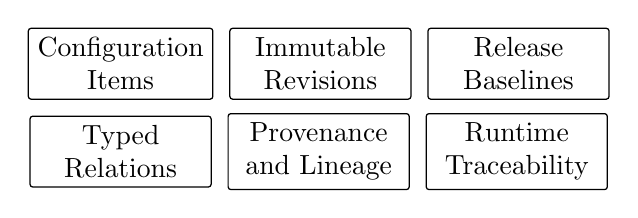
\begin{tikzpicture}[
            baseline,
            component/.style={
                draw,
                rounded corners=1pt,
                minimum width=23mm,
                minimum height=6mm,
                align=center,
                line width=0.45pt
            }
        ]
            \node[component] (aci) {Configuration\\Items};
            \node[component, right=2mm of aci] (revisions) {Immutable\\Revisions};
            \node[component, right=2mm of revisions] (baselines) {Release\\Baselines};

            \node[component, below=2mm of aci] (relations) {Typed\\Relations};
            \node[component, right=2mm of relations] (provenance) {Provenance\\and Lineage};
            \node[component, right=2mm of provenance] (runtime) {Runtime\\Traceability};
        \end{tikzpicture}
    };

    \draw[arrow] (projection) -- (acm);

    % ---------------------------------------------------------
    % Governance capabilities
    % ---------------------------------------------------------

    \node[layer, below=5mm of acm] (governance) {
        \textbf{Governance Capabilities}\\[4pt]
        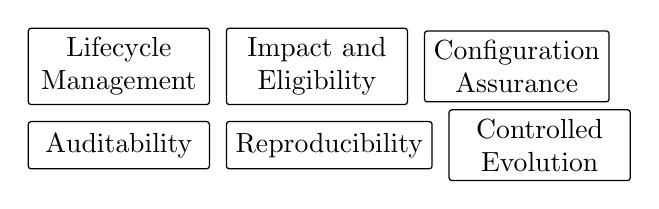
\begin{tikzpicture}[
            baseline,
            component/.style={
                draw,
                rounded corners=1pt,
                minimum width=23mm,
                minimum height=6mm,
                align=center,
                line width=0.45pt
            }
        ]
            \node[component] (lifecycle) {Lifecycle\\Management};
            \node[component, right=2mm of lifecycle] (impact) {Impact and\\Eligibility};
            \node[component, right=2mm of impact] (assurance) {Configuration\\Assurance};

            \node[component, below=2mm of lifecycle] (audit) {Auditability};
            \node[component, right=2mm of audit] (reproducibility) {Reproducibility};
            \node[component, right=2mm of reproducibility] (change) {Controlled\\Evolution};
        \end{tikzpicture}
    };

    \draw[arrow] (acm) -- (governance);

    \end{tikzpicture}

    \caption{Positioning of ACM with respect to heterogeneous agentic execution frameworks. Native configurations originating from explicit workflow graphs, metadata-driven orchestration, or delegation-based agent systems are semantically projected into a common framework-independent governance representation, allowing lifecycle management, assurance evaluation, provenance, traceability, and controlled evolution to operate independently of the originating execution framework.}
    \label{fig:acm_framework_positioning}
\end{figure}

\subsection{Contributions to Agentic Configuration Governance}
\label{sec:governance_contributions}

The contribution of ACM lies neither in introducing a new orchestration mechanism nor in extending the execution capabilities of existing agentic frameworks. Its primary contribution is to establish configuration governance as an explicit and framework-independent concern for agentic systems. From this perspective, ACM contributes at four complementary levels: representation, semantics, interoperability, and operational validation.

\subsubsection{A Framework-Independent Governance Representation}

The first contribution is a reference model that represents an agentic system as a governed configuration rather than as a collection of framework-specific runtime objects. The model introduces explicit configuration items, immutable revisions, typed relationships, provenance information, and release baselines. These abstractions provide a common vocabulary for describing the constituent elements of an agentic system and the dependencies that determine its effective configuration.

This representation extends established configuration-management principles to artifacts that are specific to agentic systems. In particular, it treats agents, prompts, tools, policies, models, workflows, and dynamically instantiated components as governable objects whose identity and evolution can be tracked independently. The resulting configuration is therefore not reduced to source code, deployment metadata, or execution traces. It is represented as an explicit and auditable object in its own right.

A central consequence of this model is the ability to distinguish logical identity from immutable revision identity. Successive revisions of the same configuration item preserve a stable conceptual identity while remaining individually addressable through exact revision identifiers and content digests. This distinction supports reproducibility, comparison, controlled replacement, and historical reconstruction without conflating an evolving artifact with one of its concrete states.

\subsubsection{Formal Governance Semantics}

The second contribution is the formalization of governance semantics over the reference model. ACM does not merely describe which artifacts exist; it defines how their governance states evolve and how local changes affect dependent configurations.

The lifecycle model specifies admissible transitions for configuration revisions, baselines, and runtime instances. Quality, assurance, impact, and eligibility are maintained as distinct dimensions rather than being collapsed into a single status. This separation prevents ambiguous interpretations such as treating a lack of evidence as proof of poor quality or propagating the lifecycle state of a dependency directly to its parent.

The propagation semantics further define how dependency changes, invalidated evidence, deprecated components, and runtime deviations influence the governance status of composite configurations. These effects are restrictive rather than destructive: a problematic dependency may block the promotion of a composite configuration without rewriting the intrinsic quality or lifecycle state of that composite. The model thereby preserves the provenance of governance decisions while supporting deterministic and explainable state computation.

The assurance model complements these semantics by linking governance conclusions to explicit evidence. Validation and approval are attached to exact revisions and scopes, allowing the system to distinguish directly assessed artifacts from conclusions inherited through assurance-relevant dependencies. Governance states can therefore be interpreted together with the evidence and rules from which they were derived.

\subsubsection{Framework-Independent Semantic Projection}

The third contribution is the separation between framework-specific extraction and framework-independent governance processing. Native configurations are translated into ACM through semantic projection, while the governance kernel operates exclusively on normalized ACM artifacts.

This architecture allows heterogeneous orchestration paradigms to be governed through a common representation. A graph-oriented framework may expose nodes and edges directly, whereas a role- and task-oriented framework may require part of its topology to be reconstructed from assignments and dependencies. ACM does not require these native representations to be structurally identical. It requires the projection to preserve the information needed for configuration governance and to make approximated or unavailable information explicit.

Framework independence should therefore be understood as independence of the governance model and processing semantics from a specific execution framework. The adapters remain framework-specific because they interpret native concepts. Once projection is complete, however, lifecycle validation, baseline construction, dependency analysis, assurance computation, runtime integration, and impact propagation no longer depend on the source framework.

This separation provides a basis for interoperability without imposing a common execution model. Frameworks retain their native orchestration semantics, while ACM supplies a shared governance representation above them.
The experimental evaluation further demonstrates that this interoperability extends beyond heterogeneous orchestration models to heterogeneous introspection regimes. The evaluated frameworks expose governance-relevant information through explicit execution graphs, metadata-assisted reconstruction, and delegation-oriented agent handoffs, respectively. By normalizing these complementary representations into a common ACM configuration graph, semantic projection isolates framework-specific extraction from governance processing, allowing identical governance semantics to be applied independently of the native introspection mechanism.

\subsubsection{Reference Operationalization and Evaluation}

The fourth contribution is the operationalization of the reference model through an executable implementation together with its experimental validation across three representative agentic frameworks. Beyond demonstrating implementability, the reference implementation provides a reproducible operational realization of the proposed governance semantics, including semantic projection, deterministic governance evaluation, runtime reconstruction, and quantitative impact analysis.

The LangGraph, CrewAI, and OpenAI Agents SDK adapters instantiate the semantic-projection boundary for three complementary execution and introspection paradigms. Their diversity does not establish universal applicability, but provides representative evidence that the ACM reference model accommodates heterogeneous configuration abstractions while preserving common governance semantics. 

The evaluation also contributes a structured validation methodology combining normative governance scenarios, automated tests, and semantic-preservation analysis. This methodology distinguishes successful representation from exact structural equivalence and records which governance-relevant properties are preserved, reconstructed, approximated, or unavailable. It therefore provides a more appropriate validation criterion for a reference model than conventional runtime-performance benchmarking. The experimental protocol further complements this qualitative validation with a dedicated quantitative assessment of deterministic impact propagation. Together, the two experimental campaigns demonstrate not only that heterogeneous configurations can be governed through a common reference model, but also that the resulting governance analyses remain reproducible and quantitatively consistent across complementary execution frameworks.

Taken together, these four contributions establish ACM as a configuration-governance abstraction positioned between agentic execution environments and higher-level operational or organizational governance processes. The reference model defines what is governed, the formal semantics define how governance states are computed, semantic projection connects heterogeneous frameworks to the model, and the reference implementation demonstrates that these mechanisms can be operationalized consistently.

\subsection{Practical Implications}
\label{sec:practical_implications}

Beyond its conceptual contribution, ACM has practical implications for the engineering and governance of agentic systems. By introducing an explicit and framework-independent configuration representation, the proposed model enables governance activities that are difficult to perform when configuration information remains fragmented across framework-specific abstractions.

The experimental evaluation indicates that these governance capabilities remain applicable across heterogeneous execution environments despite substantial differences in their native introspection mechanisms. Consequently, governance policies can be formulated over a stable configuration representation rather than being coupled to framework-specific execution abstractions. This separation is particularly important as agentic ecosystems continue to diversify and evolve.

A first implication concerns reproducibility. In current agentic ecosystems, reproducing a previous execution often requires reconstructing configurations from multiple heterogeneous artifacts, including prompts, workflow definitions, deployment parameters, runtime traces, and external resources. ACM addresses this fragmentation by associating executions with immutable configuration revisions and controlled release baselines. A governed execution can therefore be traced back to the exact configuration from which it originated, supporting reproducible experiments, regression analyses, and long-term maintenance. The experimental campaigns further indicate that reproducibility extends beyond immutable configuration snapshots. Equivalent governed representations, deterministic impact propagation, and identical governance outcomes were obtained across repeated executions and heterogeneous execution frameworks. These observations suggest that governance reproducibility depends primarily on the normalized ACM representation rather than on the native execution environment.

A second implication concerns auditability and traceability. Since governance decisions are explicitly linked to identified configuration revisions and supporting evidence, the provenance of a validation result or lifecycle transition becomes inspectable rather than implicit. This capability facilitates post-deployment analysis, compliance reporting, and forensic investigation by making configuration evolution transparent throughout the lifecycle of the system.

The explicit representation of dependencies also supports systematic change management. Instead of reasoning independently about prompts, agents, tools, or models, ACM represents these artifacts as interconnected configuration items whose relationships can be analyzed before modifications are promoted to a released baseline. Dependency-aware impact analysis provides early visibility into the potential consequences of configuration changes, reducing the likelihood of unintended regressions. The quantitative evaluation additionally suggests that governance-driven impact analysis may substantially reduce the configuration space requiring manual verification after a change. Rather than inspecting every potentially affected artifact, practitioners can focus their review on the governed impact set computed through deterministic propagation. Although the reported inspection reduction remains an experimental estimate rather than the outcome of a controlled user study, it illustrates the practical value of combining semantic dependency analysis with explicit governance relationships.


The proposed model also provides a common governance abstraction that may facilitate interoperability across heterogeneous execution environments. Organizations frequently combine multiple orchestration frameworks to address different operational requirements. By projecting these heterogeneous configurations into a shared governance representation, ACM enables governance policies to be expressed independently of the underlying execution technology while allowing each framework to preserve its native execution semantics. 
The evaluation also indicates that interoperability should not be interpreted solely as compatibility between orchestration frameworks. The successful projection of explicit workflow graphs, metadata-assisted orchestration, and delegation-based agent systems suggests that governance interoperability can also be achieved across heterogeneous introspection regimes, provided that governance-relevant semantics are preserved during semantic projection.

ACM may therefore contribute to the emerging AgentOps ecosystem by complementing existing observability and orchestration platforms with explicit configuration governance. Current operational platforms primarily focus on execution monitoring, tracing, evaluation, and operational metrics. ACM addresses a complementary concern by governing the configuration artifacts that determine how those executions are produced. Consequently, the model should be viewed as a governance layer that can coexist with, rather than replace, existing AgentOps and LLMOps infrastructures. 
From this perspective, ACM complements operational observability rather than competing with it. Execution-oriented platforms primarily describe what occurred during runtime, whereas ACM governs the configuration artifacts, dependencies, and assurance evidence that explain why a governed execution was possible. The combination of both perspectives provides a more complete governance foundation spanning configuration, execution, and evolution.

%%%%%%%%%%%%%%%%%%%%%%%%%%%%%%%%%%%%%%%%%%%%%%%%%%%%%%%%%%%%%%%%%%%%%%%%%%%%%%%%
\subsection{Limitations of the Current Reference Model}
\label{subsec:limitations}

The objective of ACM is to provide a framework-independent governance representation for the governance of agentic system configurations rather than an execution platform or an autonomous reasoning architecture. Accordingly, the current version focuses on representing governed configuration artifacts, their lifecycle, dependencies, provenance, assurance, and runtime conformance, while intentionally leaving the internal execution logic of agentic systems outside the scope of the reference model.

Table~\ref{tab:limitations_scope} summarizes the current coverage of ACM and the principal capabilities intentionally deferred to future work.

\begin{table}[t]
	\caption{Current scope of the ACM reference model.}
	\label{tab:limitations_scope}
	\centering
	\begin{tabular}{ll}
		
		\toprule
		
		Currently covered &
		Not yet covered \\
		
		\midrule
		
		Semantic projection &
		Distributed execution \\
		
		Configuration governance &
		Multi-agent planning strategies \\
		
		Immutable revision management &
		Learning and adaptation mechanisms \\
		
		Lifecycle semantics &
		Autonomous reasoning policies \\
		
		Dependency propagation &
		Self-modifying execution strategies \\
		
		Runtime provenance &
		Collective agent negotiation \\
		
		Assurance evaluation &
		Long-term memory management \\
		
		Deterministic replay &
		Continual learning \\
		
		Framework-independent governance &
		Native communication protocols (e.g., MCP, A2A) \\
		
		Cross-framework governance &
		Large-scale industrial validation \\
		
		\bottomrule
		
	\end{tabular}
	
	\end{table}

These limitations result from deliberate modeling decisions rather than technical constraints. ACM intentionally separates governance concerns from execution concerns in order to establish a stable and framework-independent governance layer. Integrating planning algorithms, reasoning strategies, learning mechanisms, or execution optimizations into the reference model would both increase its complexity and compromise the conceptual independence required for long-term interoperability.

Consequently, ACM treats reasoning engines, orchestration frameworks, planning modules, learning components, communication protocols, and other execution technologies as external systems whose observable configuration and runtime behavior can be represented and governed without prescribing their internal operation. ACM therefore specifies \emph{what} is governed---configuration revisions, baselines, dependencies, runtime observations, and assurance evidence---rather than \emph{how} autonomous agents reason, plan, negotiate, or learn.

This separation also preserves the stability of the governance model as agentic technologies evolve. New execution frameworks, orchestration paradigms, communication protocols, or reasoning techniques can be incorporated through semantic projection without modifying the governance semantics themselves. The evaluation presented in this paper should therefore be interpreted as validating the ability of ACM to represent and govern heterogeneous agentic configurations, not the correctness, efficiency, or intelligence of the underlying execution mechanisms.

Although the present evaluation demonstrates consistent governance semantics across three representative frameworks, these results should not be interpreted as establishing universal framework coverage. Additional validation across emerging execution environments, communication protocols, and industrial-scale deployments remains necessary to assess the broader applicability of the proposed governance model.

The experimental validation remains limited to the representative orchestration frameworks and configuration scales considered by the reference implementation. Although the reported results provide encouraging evidence regarding the generality of the proposed governance semantics across complementary introspection regimes, they remain confined to controlled experimental scenarios. Broader empirical validation involving additional execution frameworks, industrial-scale configurations, human-centered governance workflows, and emerging agent communication protocols will be required before stronger claims regarding general applicability can be made.

\subsection{Section Summary}

This discussion has positioned ACM as a framework-independent governance layer dedicated to the management of agentic system configurations throughout their lifecycle. Rather than introducing another orchestration framework or execution model, ACM separates governance from execution by providing a common semantic representation upon which lifecycle management, assurance evaluation, dependency analysis, provenance tracking, runtime traceability, and controlled evolution can be performed independently of the originating execution framework.

The experimental evaluation strengthens this positioning by demonstrating that the proposed governance semantics remain applicable across heterogeneous execution frameworks and complementary introspection regimes. Native configurations originating from explicit workflow graphs, metadata-assisted orchestration, and delegation-oriented agent systems are normalized through semantic projection into equivalent governed ACM representations. Together with the quantitative evaluation of deterministic impact propagation, these results indicate that governance can be expressed over a stable and framework-independent configuration model despite substantial differences in native execution abstractions.

The proposed reference model should therefore be viewed as a governance abstraction complementing existing AgentOps and agentic execution ecosystems rather than replacing them. By combining a unified configuration representation with formal governance semantics and reproducible operationalization, ACM establishes a common foundation for configuration governance while remaining intentionally independent of framework-specific orchestration mechanisms. The following section discusses the principal threats to the validity of the present study and the factors that should be considered when interpreting these results.

\section{Threats to Validity}
\label{sec:threats_validity}

The preceding sections presented the ACM reference model, its formal governance semantics, its operationalization through a reference implementation, and an experimental evaluation conducted across two heterogeneous agentic frameworks. Together, these elements provide evidence that the proposed model is internally consistent, operationally realizable, and capable of preserving governance semantics within the evaluated scope.

As with any reference model, however, these results must be interpreted within the boundaries of the assumptions, implementation choices, and experimental conditions that characterize the present study. The purpose of this section is therefore not to question the conceptual validity of ACM itself, but to identify the principal factors that may influence the interpretation, reproducibility, and generalization of the reported results.

Following established empirical research practice, we distinguish threats related to the scope of the reference model, the validation of its formal semantics, the internal validity of the experimental methodology, the external validity of the reported conclusions, and the reproducibility of the evaluation artifacts. These limitations define the current scope of evidence supporting ACM and naturally motivate the research directions discussed in the following section.

\subsection{Validity of the Reference Model}
\label{sec:validity_reference_model}

The primary objective of this study is to evaluate whether ACM provides a sufficiently expressive and framework-independent governance representation for representing and governing heterogeneous agentic system configurations. Consequently, the reported results should be interpreted as evidence supporting the proposed reference model within the scope of the evaluated frameworks rather than as a demonstration of universal applicability.

The evaluation intentionally considers three representative agentic frameworks exhibiting complementary introspection regimes. LangGraph exposes an explicit execution graph, CrewAI combines declarative orchestration with partial semantic reconstruction, whereas the OpenAI Agents SDK derives governance topology from explicit agent handoff relationships. Together, these frameworks exercise explicit introspection, partial introspection, and delegation-oriented topology reconstruction. Successfully projecting these heterogeneous representations into a common ACM configuration model provides evidence that the proposed governance abstractions are not tied to a single execution paradigm or introspection mechanism. Nevertheless, the evaluation remains limited to these three representative frameworks and should not yet be interpreted as exhaustive validation of the broader agentic ecosystem.

Other categories of agentic systems, including architectures relying on dynamic handoffs, highly decentralized coordination mechanisms, large-scale enterprise orchestration platforms, or future framework abstractions, have not yet been experimentally evaluated. Although the semantic projection architecture was explicitly designed to accommodate heterogeneous native representations, additional adapters and experimental studies are required before broader claims regarding framework independence can be established empirically.

Accordingly, the conclusions drawn from this study should be understood as demonstrating governance portability across three complementary introspection regimes rather than complete universality across every existing or future agentic framework. Additional validation across emerging execution environments, communication protocols, and industrial deployments remains necessary before stronger claims regarding general applicability can be established.


\subsection{Validity of the Formal Semantics}
\label{sec:validity_formal_semantics}

The governance semantics introduced in this work define the formal behavior of the ACM reference model through explicit lifecycle state machines, deterministic state propagation, assurance composition, and runtime governance rules. Unlike purely conceptual reference models, these semantics are operationalized by a reference implementation that executes the corresponding state computations, validation procedures, and propagation algorithms. Consequently, the reported experimental results validate not only the structural expressiveness of the reference model but also the practical executability of its governance semantics.

Nevertheless, the present study should not be interpreted as providing a formal proof of correctness of the proposed semantics. The mathematical definitions establish the intended behavior of the governance model, while the reference implementation demonstrates that these semantics can be operationalized consistently for the evaluated scenarios. This constitutes constructive evidence of correctness through implementation and experimentation rather than a formal verification of the underlying mathematical system.

Although the present work establishes formal properties including monotonicity, convergence, termination, and deterministic fixed-point computation under the assumptions of the ACM governance model, these results are derived for the reference semantics defined in this work. Extending these guarantees to future extensions of the metamodel, additional propagation policies, or independently developed implementations remains outside the scope of the present study.

Accordingly, the formal semantics should be regarded as an executable semantic specification supported by experimental evidence rather than as a mathematically verified formal system. Extending ACM with machine-checked proofs or theorem-based verification constitutes an important direction for future research and would further strengthen the theoretical foundations of the proposed governance model.

\subsection{Generalizability}
\label{sec:generalizability}

The evaluation reported in this study provides initial evidence that the ACM reference model can represent and govern heterogeneous agentic systems originating from multiple orchestration paradigms. Nevertheless, the scope of the experimental validation remains intentionally limited and should not be interpreted as demonstrating universal applicability across the rapidly evolving ecosystem of agentic frameworks.

The experimental study covers three representative frameworks spanning complementary introspection regimes. LangGraph represents explicit graph-based introspection, CrewAI combines declarative orchestration with partial semantic reconstruction, and the OpenAI Agents SDK reconstructs governance topology from explicit delegation relationships. Together, these frameworks provide broader evidence that ACM governance semantics remain applicable despite substantial differences in native observability and execution abstractions.

\begin{table}[t]
\caption{Scope of the current empirical validation and representative future validation targets.}
\label{tab:validation_scope}
\centering
\begin{tabular}{p{4.0cm}cc}
\toprule
\textbf{Agentic System Category} & \textbf{Evaluated} & \textbf{Future Work} \\
\midrule
Graph-based orchestration (LangGraph) & \checkmark & \\
Role/task-based orchestration (CrewAI) & \checkmark & \\
Dynamic handoff architectures & & \checkmark \\
Hierarchical multi-agent delegation & & \checkmark \\
Swarm-based coordination & & \checkmark \\
Pipeline-oriented orchestration & & \checkmark \\
Large-scale enterprise deployments & & \checkmark \\
Cross-organizational governance & & \checkmark \\
\bottomrule
\end{tabular}
\end{table}

Nevertheless, the evaluation does not yet include several emerging categories of agentic systems, including decentralized swarms, federated multi-agent ecosystems, large-scale industrial deployments, communication-centric architectures, or future orchestration paradigms that may expose fundamentally different governance-relevant abstractions. Consequently, the present evaluation should be interpreted as representative rather than exhaustive.

Similarly, the current experiments were conducted on normative governance scenarios and a reference implementation intended to validate the expressiveness and operational feasibility of the proposed model. They do not constitute an evaluation of industrial deployments involving thousands of configuration items, heterogeneous execution infrastructures, long-running production systems, or continuously evolving organizational governance processes.

Consequently, the conclusions of this study should be interpreted as evidence that ACM provides a viable framework-independent governance model for the classes of agentic systems evaluated, rather than as proof of universal applicability to every existing or future orchestration framework. Extending the empirical validation to additional ecosystems and deployment contexts constitutes an important direction for future work.

%%%%%%%%%%%%%%%%%%%%%%%%%%%%%%%%%%%%%%%%%%%%%%%%%%%%%%%%%%%%%%%%%%%%%%%%%%%%%%%%
\subsection{Reproducibility and Replicability}
\label{subsec:reproducibility}

Reproducibility was a primary design objective throughout the development and evaluation of ACM. To facilitate independent verification, the complete experimental protocol is defined through declarative fixtures, normative evaluation scenarios, deterministic governance rules, and an immutable event model. These artifacts enable independent implementations to evaluate the same governance properties under comparable experimental conditions.

An important characteristic of the evaluation methodology is that the
experimental scenarios are \emph{normative} rather than demonstrative. Each scenario specifies a governance property that the reference implementation is expected to verify, regardless of whether the evaluated execution represents a valid or an invalid configuration. Consequently, successful evaluation does not necessarily imply that the tested configuration is accepted by ACM; in many cases, the expected outcome is precisely the detection of a governance
violation.

Several scenarios intentionally introduce invalid lifecycle transitions, missing dependencies, unauthorized runtime behavior, or configuration drift. The correct behavior of the governance kernel is therefore to detect, classify, and report these inconsistencies according to the formal semantics defined by the reference model. From this perspective, rejecting an invalid configuration constitutes a successful execution of the corresponding normative scenario.

This distinction proved particularly valuable during the iterative development of the reference implementation. Two scenarios (ACM-S02 and ACM-S20) initially revealed inconsistencies between the normative specification and the prototype implementation. Rather than invalidating the experimental methodology, these results demonstrated its effectiveness as a validation mechanism: the observed discrepancies led to refinements of the governance semantics before completion of the evaluation campaign.

Replicability is further supported by the deterministic nature of the
governance kernel. Given identical configuration revisions, governance
policies, assurance evidence, and runtime events, repeated executions produce equivalent governance states and identical compliance decisions. This property holds independently of the probabilistic outputs generated by the underlying LLMs because ACM governs configuration and execution semantics rather than
model inference itself. This deterministic behavior is additionally supported by the quantitative impact evaluation. Nine representative impact scenarios, combining three propagation classes across the three evaluated frameworks, were each executed repeatedly under identical conditions. Across all repetitions, the governance kernel produced identical governed impact sets, identical fixed-point convergence behavior, and identical quantitative metrics. These observations provide empirical evidence that governance reproducibility depends on the normalized ACM representation and deterministic governance semantics rather than on framework-specific execution behavior.

The publication of the reference implementation, the declarative test
fixtures, the normative scenario suite, and the associated evaluation protocol allows future implementations of ACM to reproduce the experimental campaign, compare governance behaviors, and evaluate semantic equivalence independently of the original prototype. The reproducibility objective of this work is therefore not to reproduce a specific software implementation, but to enable independent verification of the governance semantics defined by the ACM reference model.
The evaluation protocol also deliberately separates semantic projection, governance computation, and experimental instrumentation. Measurement components observe the governed representations produced by the governance kernel without participating in governance state computation. This architectural separation reduces the risk that evaluation artifacts influence the semantics being evaluated and contributes to the reproducibility of the reported results.

\begin{figure}[t]
    \centering
    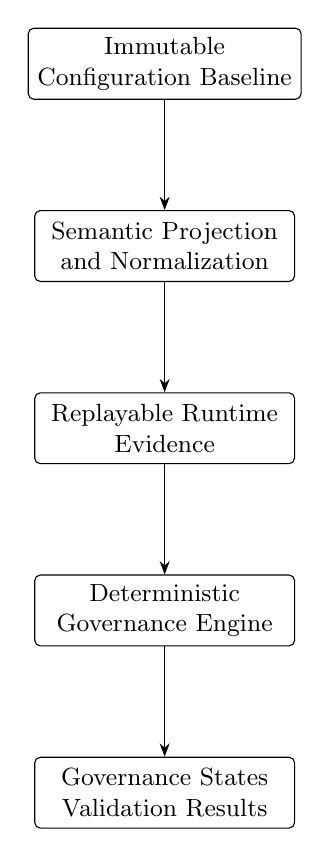
\begin{tikzpicture}[
    node distance=1.4cm,
    >=Stealth,
    box/.style={
        draw,
        rounded corners=2pt,
        align=center,
        minimum width=3.3cm,
        minimum height=0.9cm,
        font=\small
    }
]

\node[box] (baseline) {Immutable\\Configuration Baseline};

\node[box, below=of baseline] (projection) {Semantic Projection\\and Normalization};

\node[box, below=of projection] (runtime) {Replayable Runtime\\Evidence};

\node[box, below=of runtime] (engine) {Deterministic\\Governance Engine};

\node[box, below=of engine] (results) {Governance States\\Validation Results};

\draw[->] (baseline) -- (projection);
\draw[->] (projection) -- (runtime);
\draw[->] (runtime) -- (engine);
\draw[->] (engine) -- (results);

\end{tikzpicture}
    \caption{Deterministic governance pipeline supporting reproducibility and replicability. Immutable configuration baselines, semantic projection, replayable runtime evidence, and deterministic governance computation together enable independent reproduction of governance results without requiring deterministic LLM outputs.}
    \label{fig:reproducibility_pipeline}
\end{figure}

\subsection{Mitigation Strategies}
\label{sec:mitigation_strategies}

Although the preceding subsections identify several limitations affecting the present study, a number of methodological choices were deliberately adopted to reduce their impact on the reported results. Rather than attempting to maximize the breadth of the evaluation, the experimental methodology emphasizes internal consistency, deterministic governance semantics, and explicit separation between conceptual modeling, operationalization, and experimental validation.

First, the reference model was intentionally designed independently of any particular execution framework. The semantic projection architecture isolates framework-specific extraction mechanisms from the governance kernel, allowing the latter to remain unchanged across heterogeneous orchestration paradigms. This separation reduces implementation bias and facilitates the extension of the evaluation to additional frameworks without modifying the underlying governance semantics.

Second, the evaluation relies on normative governance scenarios rather than application-specific benchmarks. Each scenario targets a well-defined property of the reference model, such as lifecycle management, dependency propagation, assurance computation, baseline validation, or runtime governance. This scenario-driven methodology improves the traceability between the formal specification, the reference implementation, and the experimental evidence.

Third, reproducibility is reinforced through deterministic governance computation, immutable configuration revisions, canonical serialization, replayable runtime evidence, and automated validation procedures. These mechanisms ensure that governance outcomes depend exclusively on governed configurations and observed runtime events rather than on the stochastic behavior of the underlying language models.

In conclusion, this article deliberately distinguishes between the conceptual reference model, its formal governance semantics, the reference implementation, and the experimental evaluation. This separation avoids conflating theoretical contributions with implementation artifacts and allows future implementations to validate the same governance semantics independently of the current prototype.

Table~\ref{tab:mitigation_strategies} summarizes the principal threats identified in this section together with the corresponding mitigation strategies adopted throughout the study.

\begin{table}[t]
\caption{Summary of Threats and Mitigation Strategies}
\label{tab:mitigation_strategies}
\centering
\begin{tabular}{p{4.2cm}p{3.9cm}}
\toprule
\textbf{Threat} & \textbf{Mitigation Strategy} \\
\midrule
Limited coverage of currently evaluated introspection regimes &
Evaluation across heterogeneous orchestration paradigms; framework-independent governance kernel. \\

Incomplete formal verification &
Executable formal semantics supported by deterministic implementation and normative validation scenarios. \\

Limited empirical generalization &
Conservative interpretation of results; explicit delimitation of the evaluation scope. \\

Implementation-dependent bias &
Separation between semantic projection, governance kernel, and framework adapters. \\

Experimental reproducibility &
Immutable revisions, replayable runtime events, canonical serialization, and automated validation suite. \\

Emerging agentic architectures &
Projection architecture designed to accommodate additional adapters without modifying the reference model. \\

Experimental instrumentation bias &
Strict separation between semantic projection, governance computation, and experimental instrumentation; evaluation artifacts remain external to the governance kernel. \\

Experimental instrumentation coupling &
Strict architectural separation between semantic projection, governance computation, and evaluation instrumentation prevents experimental measurements from influencing governed state computation. \\

\bottomrule
\end{tabular}
\end{table}

\subsection{Section Summary}
\label{sec:threats_summary}

The objective of this section has been to delimit the scope within which the conclusions of the present study should be interpreted. The identified threats do not challenge the internal consistency of the ACM reference model nor the coherence of its governance semantics. Instead, they primarily concern the breadth of the experimental validation, the current level of formal verification, and the extent to which the reported results can be generalized across the rapidly evolving landscape of agentic systems.

The experimental methodology intentionally favors methodological rigor over exhaustive coverage by combining a framework-independent governance representation, executable governance semantics, deterministic validation procedures, and reproducible experimental artifacts. Within this scope, the reported results provide credible evidence supporting the feasibility and expressiveness of the proposed governance model while avoiding claims that extend beyond the evaluated configurations.

These limitations should therefore be interpreted as defining the current scope of empirical evidence rather than indicating inconsistencies in the proposed governance model. Within this scope, the combination of formal semantics, deterministic operationalization, qualitative validation, and quantitative impact evaluation provides consistent evidence supporting the feasibility of framework-independent governance for heterogeneous agentic systems. The remaining limitations primarily concern the breadth of empirical validation and the progressive extension of the reference model to the rapidly evolving agentic ecosystem.

\section{Future Work}
\label{sec:future_work}

The ACM reference model introduced in this paper constitutes an initial step toward a framework-independent approach to the governance of agentic systems. The proposed metamodel, governance semantics, reference implementation, and experimental evaluation collectively demonstrate the feasibility of this approach within the scope considered in the present study. At the same time, the limitations identified in the previous section highlight several opportunities for extending both the theoretical foundations and the practical applicability of ACM.

Future research therefore naturally follows three complementary directions. The first concerns the evolution of the reference model itself to accommodate emerging abstractions while preserving its governance principles. The second focuses on strengthening the empirical and theoretical validation of the proposed semantics through broader experimental studies and formal verification. The long-term perspective is to position ACM as a common governance layer capable of interoperating with the rapidly expanding ecosystem of agentic development, deployment, and observability platforms.

\subsection{Extension of the Reference Model}
\label{sec:future_reference_model}

The reference model presented in this paper intentionally focuses on the minimal set of governance concepts required to represent heterogeneous agentic systems independently of their execution framework. This design choice favors conceptual stability and limits the number of core abstractions to those introducing distinct governance semantics. Nevertheless, the rapid evolution of agentic ecosystems will inevitably lead to the emergence of new configuration artifacts, interaction patterns, and execution abstractions that may require additional modeling capabilities.

A primary direction for future research is therefore the controlled evolution of the ACM metamodel while preserving its foundational design principles. Rather than continuously introducing framework-specific concepts into the core model, future extensions should remain guided by semantic necessity: a new abstraction should only become part of the reference model if it introduces governance properties that cannot be represented through the existing concepts and relationships. This principle preserves the framework independence of ACM while avoiding unnecessary growth of the metamodel.

The experimental evaluation reported in this work provides an initial empirical basis for this extension strategy. By successfully projecting three representative frameworks spanning complementary introspection regimes into a common governance representation, the current results suggest that future extensions should primarily address genuinely new governance abstractions rather than framework-specific implementation differences.

An important example concerns reusable composite capabilities that are increasingly appearing under different names across modern agentic platforms, such as skills, reusable workflows, capability modules, or packaged execution components. Although these constructs differ in their implementation details, they frequently encapsulate existing governed artifacts—including prompts, tools, models, policies, workflows, and external resources—rather than introducing fundamentally new governance semantics. Consequently, many of these emerging abstractions can already be represented through semantic projection as governed composite configuration items without requiring modifications to the ACM core.

An important direction concerns the governance of increasingly composite AI systems, including Retrieval-Augmented Generation (RAG) pipelines and other retrieval-centric architectures. Rather than introducing a dedicated governance abstraction, ACM can represent RAG pipelines through the composition of existing configuration items, including embedding models, retrieval policies, vector indexes, knowledge repositories, prompt definitions, and retrieval components. This representation enables immutable versioning of the complete retrieval configuration, explicit provenance of derived vector indexes, and governance of retrieval policies independently of the underlying storage technology. Consequently, ACM can govern the evolution of retrieval-augmented systems without embedding retrieval-specific concepts into its core metamodel.

Another important direction concerns self-learning or continuously adaptive agents. Such systems challenge traditional configuration management because parts of their operational behavior may evolve autonomously through accumulated experience, parameter adaptation, or long-term memory updates. Extending ACM to distinguish immutable governed configurations from controlled runtime knowledge evolution would enable adaptive systems to remain auditable while preserving reproducibility of approved configurations. Future work should therefore investigate governance semantics capable of representing learning artifacts, adaptation boundaries, and evidence associated with autonomous configuration evolution.

Finally, the increasing adoption of interoperability protocols and workflow orchestration platforms, including Model Context Protocol (MCP), Agent-to-Agent (A2A) communication, and low-code orchestration environments such as n8n, provides another opportunity for extending the reference model. Rather than incorporating protocol-specific abstractions, ACM can represent these ecosystems through semantic projection of communication endpoints, external services, orchestration workflows, and interaction contracts into governed configuration items. This approach preserves the framework-independent nature of the reference model while enabling configuration governance across heterogeneous execution environments and emerging interoperability standards.

Future extensions may also address governance capabilities that extend beyond the scope of the current reference model. Examples include distributed governance across multiple organizations, federated configuration repositories, cross-system dependency management, richer policy composition mechanisms, and governance of long-lived autonomous ecosystems whose configuration evolves continuously over time. These extensions would broaden the applicability of ACM while preserving the separation between configuration governance and execution that constitutes one of its central architectural principles.

Ultimately, the long-term evolution of ACM should prioritize conceptual stability over feature accumulation. As with mature reference models in software engineering, the objective is not to mirror every innovation introduced by individual frameworks, but rather to identify the stable governance abstractions that remain applicable despite the continuous evolution of execution technologies. This philosophy enables the reference model to evolve incrementally while maintaining interoperability, explainability, and long-term sustainability.

\subsection{Broader Framework Validation}
\label{sec:future_framework_validation}

The empirical evaluation presented in this paper intentionally focuses on two representative orchestration paradigms in order to demonstrate the feasibility of framework-independent configuration governance. Although the successful semantic projection of LangGraph and CrewAI provides encouraging evidence supporting the proposed reference model, broader validation across the rapidly evolving landscape of agentic systems remains an essential research direction.

Future work should therefore prioritize the evaluation of additional classes of agentic architectures rather than merely increasing the number of supported execution frameworks. The objective is to determine whether fundamentally different governance-relevant abstractions require extensions of the semantic projection contract or can be represented using the existing ACM concepts. In particular, architectures relying on dynamic delegation, decentralized collaboration, communication-centric coordination, adaptive execution, or large-scale distributed governance, would provide valuable opportunities to evaluate the expressiveness of the ACM metamodel under substantially different execution models.

Beyond execution frameworks themselves, validation could also incorporate complementary components of the emerging AgentOps and LLMOps ecosystem. Provenance platforms, observability infrastructures, evaluation frameworks, and deployment management systems increasingly expose governance-relevant metadata that could naturally participate in semantic projection. Studying the integration of ACM with such platforms would provide additional evidence regarding the ability of the reference model to serve as a common governance layer across heterogeneous operational environments.

Another important direction concerns empirical validation at industrial scale. The current experiments intentionally emphasize semantic correctness rather than operational scalability. Future studies should therefore evaluate ACM on large agentic systems involving hundreds or thousands of governed configuration items, long-lived execution histories, continuously evolving baselines, and collaborative governance processes distributed across multiple development teams. Such evaluations would provide quantitative evidence regarding scalability, governance overhead, and operational usability in realistic production environments.

Ultimately, extending the experimental validation is not intended merely to increase the number of supported frameworks. Rather, it aims to progressively strengthen the empirical evidence supporting the central hypothesis of this work: that governance semantics can remain stable despite the continuous evolution of agentic execution technologies.

The current evaluation already indicates that governance portability extends across three complementary introspection regimes. Future validation should therefore progressively investigate whether this portability also extends across new architectural families, organizational scales, and interoperability mechanisms.

\subsection{Formal Verification of Governance Semantics}
\label{sec:future_formal_verification}

The governance semantics introduced in this paper are defined through a formal operational specification and validated through deterministic execution of the reference implementation.While this approach establishes formal properties for the governance semantics and demonstrates their operational realizability through the reference implementation, it does not yet provide machine-assisted verification of the complete governance model.

One immediate objective concerns the verification of the fixed-point propagation algorithm underlying governance state computation. Formal proofs could establish properties such as termination, determinism, convergence toward a unique governance state, and independence from evaluation order. Demonstrating these properties would strengthen confidence that governance decisions remain stable regardless of implementation details or execution strategies.

A second research direction involves the formal analysis of the lifecycle semantics themselves. The lifecycle state machines, dependency propagation rules, assurance composition mechanisms, and runtime governance semantics could be expressed within a formal verification framework in order to prove invariants such as transition consistency, absence of contradictory governance states, preservation of dependency constraints, and correctness of state propagation under arbitrary configuration topologies.

Beyond individual algorithms, future work may investigate the formal specification of the ACM reference model as a complete governance system. Model-checking techniques, temporal logic, theorem proving, or specification languages dedicated to distributed systems could be employed to verify global properties of the governance semantics and to detect inconsistencies automatically during the evolution of the reference model. Such approaches would complement the current implementation-based validation with machine-verifiable correctness guarantees.

Formal verification would facilitate the development of independent ACM implementations. By providing mathematically specified governance semantics rather than relying solely on behavioral equivalence with the reference implementation, future implementations could demonstrate conformance through proof of semantic equivalence instead of implementation similarity. This evolution would represent an important step toward establishing ACM as a stable and implementation-independent governance specification.

\subsection{Toward an Agentic Configuration Ecosystem}
\label{sec:future_ecosystem}

The rapid maturation of agentic software engineering has led to the emergence of a rich ecosystem of complementary technologies dedicated to development, deployment, observability, evaluation, provenance, and operational governance. Rather than replacing these existing technologies, ACM is intended to provide a framework-independent governance layer capable of connecting heterogeneous execution frameworks, observability platforms, evaluation systems, and software engineering infrastructures through a common semantic representation of governed configuration artifacts. The experimental results presented in this work provide initial evidence that such a governance layer can remain stable despite heterogeneous execution models and complementary introspection regimes.

\begin{figure}[t]
	\centering
	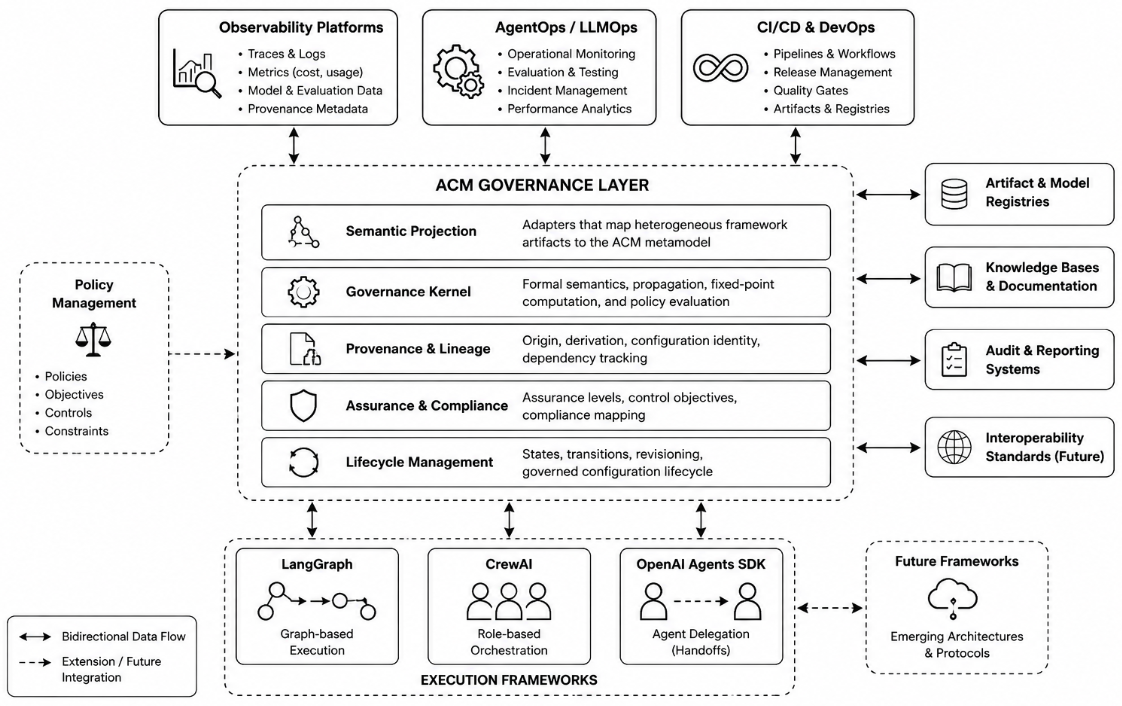
\includegraphics[width=0.8\textwidth]{figures/acm_agentic_ecosystem.png}
	\caption{Conceptual positioning of ACM within an agentic configuration ecosystem. Heterogeneous execution frameworks are connected to a common governance layer through semantic projection. This layer provides configuration governance services that interact with AgentOps platforms, software engineering infrastructures, deployment pipelines, observability systems, and future interoperability standards while remaining independent of execution technologies.}
	\label{fig:agentic_configuration_ecosystem}
\end{figure}

A promising direction for future research therefore consists in studying the integration of ACM with broader AgentOps and LLMOps ecosystems. Modern observability platforms increasingly collect execution traces, evaluation results, model usage metrics, cost information, and provenance metadata that constitute valuable inputs for governance processes. Conversely, governance decisions produced by ACM could enrich these platforms with lifecycle status, assurance levels, configuration lineage, dependency analysis, and compliance information, providing a higher semantic level for operational monitoring. This separation also enables governance policies to evolve independently from execution technologies. As orchestration frameworks continue to diversify, governance services built upon ACM could remain stable while semantic projection adapters evolve to accommodate new execution abstractions.

Rather than exchanging framework-specific metadata directly, these heterogeneous systems could interoperate through governed ACM representations that preserve configuration identity, provenance, lifecycle semantics, and assurance information independently of the originating execution technology.

Another important perspective concerns the integration of ACM with software engineering infrastructures. Continuous integration and deployment pipelines, software configuration management systems, artifact repositories, and supply-chain security mechanisms already manage the lifecycle of conventional software assets. Extending these infrastructures to incorporate governed agentic configuration items would enable unified governance across both traditional software components and AI-native artifacts while preserving traceability throughout the complete development lifecycle. Such integration would extend configuration governance beyond software artifacts alone by enabling AI-native configuration items to participate in existing software engineering governance processes while preserving immutable revision identity and reproducible configuration baselines.

Beyond tooling integration, future work may explore the definition of interoperable framework-independent governance services exposing standardized interfaces for semantic projection, configuration validation, governance state computation, and provenance exchange. Such services would facilitate the development of heterogeneous toolchains in which execution frameworks, observability platforms, deployment systems, and governance engines cooperate while remaining independently evolvable.

Ultimately, the long-term objective is not to establish ACM as another execution platform, but to provide a stable governance substrate upon which heterogeneous execution frameworks, AgentOps platforms, software engineering infrastructures, and future interoperability standards can progressively converge. As the agentic ecosystem continues to evolve, such a framework-independent governance layer may facilitate reproducibility, interoperability, auditability, and controlled evolution without constraining innovation in execution technologies.

\subsection{Standardization Perspectives}
\label{sec:future_standardization}

The absence of a common vocabulary and shared governance abstractions currently represents one of the principal obstacles to interoperability across agentic systems. While execution frameworks continue to evolve rapidly, equivalent concepts are frequently described using framework-specific terminology, making configuration exchange, governance portability, and comparative evaluation unnecessarily difficult.

The ACM reference model represents an initial step toward addressing this fragmentation by proposing a framework-independent governance vocabulary together with formally defined governance semantics and an operational reference implementation. The experimental validation further demonstrates that these concepts remain applicable across heterogeneous execution frameworks and complementary introspection regimes without requiring framework-specific governance semantics. Although the present work does not aim to establish a standard, it provides a structured foundation upon which future community discussions regarding interoperable governance models may build.

Future research may therefore investigate the definition of standardized exchange formats for governed configuration items, semantic projection interfaces, governance evidence, provenance information, and lifecycle metadata. Such specifications would facilitate interoperability between heterogeneous execution frameworks while allowing governance information to remain portable independently of implementation technologies. Likewise, standardized conformance criteria could enable independent implementations to demonstrate governance semantic compatibility with the ACM reference model while preserving implementation freedom. Such specifications would also facilitate independent implementations capable of exchanging governed configuration artifacts while preserving provenance, lifecycle semantics, assurance evidence, and reproducibility across heterogeneous governance environments.

The maturation of ACM may also benefit from collaboration with broader software engineering and artificial intelligence communities working on software configuration management, software supply-chain security, provenance, and AI governance. Aligning ACM with existing standards whenever appropriate would facilitate its integration into established engineering practices while reducing duplication of concepts that are already well understood in adjacent disciplines.

Ultimately, the long-term objective is not to standardize a particular implementation or execution framework, but to encourage convergence toward a common governance reference model for heterogeneous agentic systems. By separating governance semantics from execution technologies while validating this separation across complementary orchestration paradigms and introspection regimes, ACM provides a stable conceptual foundation upon which interoperable governance specifications may progressively emerge. Such convergence could strengthen reproducibility, auditability, configuration portability, and long-term sustainability across an increasingly diverse agentic ecosystem.

\subsection*{Section Summary}

Taken together, these research directions outline a progressive evolution of ACM rather than a redefinition of its core principles. Future work primarily concerns extending empirical validation to additional architectural classes, strengthening formal guarantees, integrating ACM within broader software engineering and AgentOps ecosystems, and fostering interoperable governance specifications. Throughout these developments, the central objective remains unchanged: preserving a stable, framework-independent governance model while enabling the continuous evolution of agentic execution technologies.

\section{Conclusion}
\label{sec:conclusion}

The rapid evolution of agentic software engineering has fundamentally transformed the role of configuration artifacts. Prompts, tools, execution graphs, policies, models, runtime state, and provenance have become first-class engineering assets whose governance can no longer rely solely on traditional software configuration management practices. At the same time, the increasing diversity of orchestration frameworks has introduced heterogeneous configuration abstractions, making governance difficult to reproduce, audit, and compare across platforms.

This paper introduced Agentic Configuration Management (ACM), a framework-independent governance model for heterogeneous agentic systems. Rather than proposing another execution framework, ACM separates governance semantics from execution technologies through a unified representation of governed configuration items, immutable revisions, semantic projection, deterministic governance semantics, assurance evaluation, and runtime traceability.

Beyond the conceptual contribution, this work demonstrated that the proposed governance semantics can be operationalized through an executable reference implementation and evaluated across three representative agentic frameworks spanning complementary introspection regimes. The experimental results show that heterogeneous configurations can be semantically projected into equivalent governed ACM representations while preserving governance-relevant information required for deterministic lifecycle evaluation, assurance computation, and impact propagation. The complementary qualitative and quantitative evaluation campaigns provide consistent empirical evidence supporting the feasibility and reproducibility of framework-independent governance for heterogeneous agentic systems.

More broadly, this work argues that governance should become an explicit architectural layer of agentic software engineering rather than an implementation-specific concern embedded within individual execution frameworks. By separating governance from execution through a common reference model, formal governance semantics, and framework-independent operationalization, ACM establishes a foundation upon which interoperability, reproducibility, auditability, controlled evolution, and future governance standards can progressively be built.

Ultimately, ACM does not prescribe how agentic systems should reason or execute; it specifies how their configurations can be governed consistently throughout their lifecycle. As execution technologies continue to evolve, the long-term value of ACM lies in providing a stable governance foundation capable of remaining independent of changing orchestration paradigms while supporting reproducibility, provenance, interoperability, assurance, and controlled configuration evolution. Such a separation between execution and governance may ultimately become a fundamental architectural principle for engineering trustworthy agentic systems.

%%%%%%%%%%%%%%%%%%%%%%%%%%%%%%%%%%%%%%%%%%%%%%%%%%%%%%%%%%%%%%%%%%%%%%%%%%%%%%%%
\appendices

\section{Related Work}
\label{appendix:related_work}
\subsubsection{Framework Comparison}
Table~\ref{tab:framework_comparison} summarizes representative characteristics of several widely used agentic frameworks.
\begin{table*}[t]
	\centering
	\caption{Representative characteristics of widely used agentic frameworks. The comparison illustrates the diversity of execution paradigms while highlighting the absence of a common configuration representation.}
	\label{tab:framework_comparison}
	
	\renewcommand{\arraystretch}{1.15}
	
	\begin{tabular}{p{3.2cm}p{3.1cm}p{3.4cm}p{3.4cm}c}
		\toprule
		\textbf{Framework}
		&
		\textbf{Primary Paradigm}
		&
		\textbf{Execution Model}
		&
		\textbf{Native Configuration Abstraction}
		\\
		\midrule
		
		LangGraph
		&
		State graph
		&
		Explicit graph execution
		&
		Nodes, edges and shared state
		\\
		
		CrewAI
		&
		Role-based multi-agent
		&
		Agents, tasks and crews
		&
		Agents, tasks, crews and flows
		\\
		
		OpenAI Agents SDK
		&
		Delegation-based agents
		&
		Handoffs and tool orchestration
		&
		Agents, tools and handoffs
		\\
		
		Microsoft Agent Framework
		&
		Workflow orchestration
		&
		Agent workflows
		&
		Workflow definitions
		\\
		
		Google ADK
		&
		Hierarchical agents
		&
		Multi-agent orchestration
		&
		Agent hierarchies
		\\
		
		\bottomrule
	\end{tabular}
	
\end{table*}
\subsection{Gap Analysis}
The Table ~\ref{tab:gap_analysis_detailed} supports a comparative gap analysis between the different governance aproaches.
\begin{table*}[t]
	\centering
	\caption{Detailed rationale supporting the comparative gap analysis
		presented in Table~\ref{tab:gap_analysis}.}
	\label{tab:gap_analysis_detailed}
	
	\footnotesize
	\setlength{\tabcolsep}{3pt}
	\renewcommand{\arraystretch}{1.18}
	
	\begin{tabularx}{\textwidth}{
			>{\RaggedRight\arraybackslash}p{3.25cm}
			C{1.05cm}
			C{1.15cm}
			C{1.45cm}
			C{1.30cm}
			C{0.85cm}
			Y
		}
		\toprule
		
		\textbf{Governance capability}
		&
		\makecell{\textbf{SCM}}
		&
		\makecell{\textbf{AI}\\\textbf{Gov.}}
		&
		\makecell{\textbf{LLMOps /}\\\textbf{AgentOps}}
		&
		\makecell{\textbf{Agent}\\\textbf{frameworks}}
		&
		\makecell{\textbf{ACM}}
		&
		\textbf{Rationale}
		\\
		
		\midrule
		
		Configuration identification
		&
		$\checkmark$
		&
		$\sim$
		&
		$\sim$
		&
		$\sim$
		&
		$\checkmark$
		&
		SCM explicitly identifies configuration items.
		Other approaches identify only the artefacts relevant to their
		respective governance, operational, or execution objectives.
		ACM represents heterogeneous artefacts as governed ACI revisions.
		\\
		
		Version management
		&
		$\checkmark$
		&
		--
		&
		$\sim$
		&
		$\sim$
		&
		$\checkmark$
		&
		SCM provides mature version control.
		LLMOps platforms and agent frameworks version selected artefacts,
		such as prompts or workflows, but not complete governed
		configurations.
		ACM assigns immutable revisions to every governed artefact.
		\\
		
		Configuration provenance
		&
		$\sim$
		&
		$\checkmark$
		&
		$\checkmark$
		&
		$\sim$
		&
		$\checkmark$
		&
		SCM preserves software history, while AI governance and LLMOps
		emphasize provenance, accountability, and traceability.
		Frameworks expose partial execution provenance.
		ACM links configuration, revision, runtime, and evidence provenance.
		\\
		
		Dependency traceability
		&
		$\checkmark$
		&
		$\sim$
		&
		$\checkmark$
		&
		$\sim$
		&
		$\checkmark$
		&
		SCM manages software dependencies, and LLMOps relates selected
		artefacts such as prompts, traces, and evaluations.
		Frameworks expose dependencies through native abstractions.
		ACM explicitly models typed dependencies across heterogeneous
		configuration artefacts.
		\\
		
		Execution observability
		&
		--
		&
		$\sim$
		&
		$\checkmark$
		&
		$\checkmark$
		&
		$\checkmark$
		&
		Execution monitoring is not a primary SCM capability.
		AI governance recommends monitoring, whereas LLMOps platforms and
		agent frameworks provide traces and runtime telemetry.
		ACM incorporates normalized runtime observations into its governance
		representation.
		\\
		
		Lifecycle governance
		&
		$\sim$
		&
		$\checkmark$
		&
		$\sim$
		&
		$\sim$
		&
		$\checkmark$
		&
		SCM governs controlled software evolution, and AI governance defines
		processes across the AI lifecycle.
		Operational platforms and frameworks mainly address deployment or
		execution stages.
		ACM governs the lifecycle of exact configuration revisions.
		\\
		
		Framework-independent representation
		&
		--
		&
		--
		&
		--
		&
		--
		&
		$\checkmark$
		&
		Existing approaches remain centred on software artefacts,
		organizational processes, operational platforms, or native execution
		models.
		ACM provides a framework-independent representation of governed
		agentic configurations.
		\\
		
		Unified configuration model
		&
		--
		&
		--
		&
		--
		&
		--
		&
		$\checkmark$
		&
		No other family combines heterogeneous artefacts, immutable
		revisions, typed dependencies, governance semantics, and runtime
		traceability within one reference model.
		This integration constitutes ACM's primary contribution.
		\\
		
		\bottomrule
	\end{tabularx}
	
	\vspace{0.4em}
	
	{\scriptsize
		$\checkmark$ Fully addressed
		\hspace{1em}
		$\sim$ Partially addressed
		\hspace{1em}
		-- Not provided as a primary capability.
	}
	
\end{table*}
	

\section{Formal Foundations}
\label{appendix:formal_foundations}

This appendix provides the mathematical definitions supporting the governance semantics introduced in Section~\ref{sec:governance_semantics}. It complements the normative presentation without introducing additional governance concepts.

\subsection{Configuration Graph}
The ACM reference model is organized as the multi-graph structure defined in Equation~(\ref{eq:acm_multigraph_structure}). The governance semantics in this appendix operate on the finite directed Configuration Graph

\begin{equation}
	G_C=(V_C,E_C),
	\label{eq:graph_definition}
\end{equation}

where:

\begin{itemize}
	\item $V_C$ denotes the finite set of immutable ACI revisions represented in the governed configuration;
	\item $E_C\subseteq V_C\times V_C\times T_R$ denotes the finite set of typed configuration relationships;
	\item $T_R$ is the finite set of relationship types defined by the reference metamodel.
\end{itemize}
The graph topology remains immutable for a given revision set. Configuration evolution is represented by introducing new immutable revisions rather than modifying existing vertices.

\subsection{Governance Descriptor}

Each configuration revision $v\in V_C$ is associated with the intrinsic
configuration governance descriptor

\begin{equation}
	\Gamma_C(v)=
	\left(
	L(v),
	Q(v),
	A(v),
	I(v),
	El(v)
	\right),
	\label{eq:descriptor_definition}
\end{equation}

whose components belong to the five configuration governance state spaces.
Runtime state is defined separately on runtime entities in $V_R$.

The configuration governance descriptor represents the intrinsic governance status of an ACI revision and introduces no computational semantics. The complete governance view additionally includes the runtime view $\rho(v)$ defined in Equation~(\ref{eq:runtime_view}).

All semantic computations are defined through dedicated evaluation functions introduced later in this appendix.

\subsection{Notation}

Throughout the remainder of this appendix, configuration governance state assignments are defined over configuration revisions:

\begin{equation}
	X:V_C\rightarrow\mathcal{X},
	\label{eq:state_assignment}
\end{equation}

where $\mathcal{X}$ denotes one of the configuration governance state spaces
$\mathcal{L}$, $\mathcal{Q}$, $\mathcal{A}$, $\mathcal{I}$, or $\mathcal{E}$.

Runtime state follows a distinct assignment $Rt:V_R\rightarrow\mathcal{R}$ because runtime entities and configuration revisions belong to different graph domains.

For propagation reasoning, an impact valuation is a state assignment

\begin{equation}
	\iota : V \rightarrow \mathcal{I},
	\label{eq:impact_valuation}
\end{equation}

where $\iota(v)$ denotes the propagated impact state associated with revision
$v$. For a fixed configuration graph, the set of all impact valuations is

\begin{equation}
	\mathcal{D}_{G}
	=
	\mathcal{I}^{V}.
	\label{eq:impact_valuation_domain}
\end{equation}

The graph structure and the propagation-policy mapping remain fixed during one
propagation computation. Only the impact valuation evolves.

\section{Governance State Spaces}
\label{appendix:state_spaces}

This appendix formally defines the state spaces introduced in
Section~\ref{sec:governance_state_spaces}. Lifecycle, quality, assurance, impact, and eligibility are configuration governance state spaces defined over $V_C$, whereas runtime is an execution state space defined over $V_R$.

\subsection{Lifecycle}

The lifecycle state space is defined as

\begin{equation}
	\mathcal{L}=
	\{
	Draft,
	Validated,
	Approved,
	Released,
	Deprecated,
	Archived
	\}.
	\label{eq:lifecycle_space}
\end{equation}

The ordering relation is the monotonic lifecycle order introduced in Equation~(\ref{eq:lifecycle_order}).

---

\subsection{Quality}

The quality state space is defined as

\begin{equation}
	\mathcal{Q}=
	\{
	Undefined,
	Valid,
	Warning,
	Invalid
	\}.
	\label{eq:quality_space}
\end{equation}

The quality state reflects the intrinsic validation status of an individual revision independently of its dependencies.

---

\subsection{Assurance}

The assurance state space is defined as

\begin{equation}
	\mathcal{A}=
	\{
	Unassessed,
	Partial,
	Satisfied
	\}.
	\label{eq:assurance_space}
\end{equation}

The assurance state represents the availability of governance evidence associated with a revision.

The corresponding ordering relation is

\begin{equation}
	Unassessed
	<
	Partial
	<
	Satisfied.
	\label{eq:assurance_order}
\end{equation}

---

\subsection{Impact}

The impact state space is defined as

\begin{equation}
	\mathcal{I}=
	\{
	None,
	Local,
	Propagated
	\}.
	\label{eq:impact_space}
\end{equation}

The impact space is equipped with the total order

\begin{equation}
	None
	\prec_{\mathcal I}
	Local
	\prec_{\mathcal I}
	Propagated.
	\label{eq:impact_order}
\end{equation}

Its least element is

\begin{equation}
	\bot_{\mathcal{I}}
	=
	None.
	\label{eq:impact_bottom}
\end{equation}

The least upper bound of two impact states is defined by

\begin{equation}
	i_1
	\sqcup_{\mathcal{I}}
	i_2
	=
	\max\nolimits_{\prec_{\mathcal{I}}}
	\left(i_1,i_2\right).
	\label{eq:impact_join}
\end{equation}

Consequently,
$\left(\mathcal{I},\preceq_{\mathcal{I}}\right)$ is a finite lattice.

The impact state identifies whether a revision has been affected by a propagated governance change.
---

\subsection{Eligibility}

The eligibility state space is defined as

\begin{equation}
	\mathcal{E}=
	\{
	Blocked,
	Restricted,
	Eligible
	\}.
	\label{eq:eligibility_space}
\end{equation}

The corresponding ordering relation is

\begin{equation}
	Blocked
	<
	Restricted
	<
	Eligible.
	\label{eq:eligibility_order}
\end{equation}

The eligibility state summarizes whether a revision satisfies the governance conditions required for operational use.

---

\subsection{Runtime}

The runtime state space is defined as

\begin{equation}
	\mathcal{R}=
	\{
	Created,
	Ready,
	Running,
	Waiting,
	Completed,
	Failed,
	Cancelled,
	Terminated
	\}.
	\label{eq:runtime_space}
\end{equation}

The runtime state represents the execution status reconstructed from runtime observations independently of the configuration lifecycle.

Unlike the previous state spaces, runtime states are reconstructed from execution events rather than assigned through governance decisions.

Accordingly, runtime state is assigned to runtime entities rather than
configuration revisions:

\begin{equation}
	Rt:V_R\rightarrow\mathcal{R}.
	\label{eq:runtime_state_assignment}
\end{equation}

\section{Propagation Policies}
\label{appendix:propagation_policies}

This appendix formally defines the propagation policies introduced in Section~\ref{sec:propagation_policies}. Propagation policies characterize how governance information traverses configuration relationships independently of the governance state evaluation.

\subsection{Policy Space}

Let $T_R$ denote the finite set of relationship types defined by the ACM reference model.

Each configuration relationship is associated with exactly one propagation policy through the resolved policy view

\begin{equation}
	\Pi:E_C\rightarrow\mathcal P,
\end{equation}

where the policy space is defined as

\begin{equation}
	\mathcal{P}=
	\left\{
	\textit{Blocking},
	\textit{Warning},
	\textit{Informational},
	\textit{None}
	\right\}.
	\label{eq:policy_set}
\end{equation}

A propagation policy is declarative: it does not itself modify an impact state. Instead, it selects the impact-transfer semantics applied when propagation traverses a governed configuration relationship.
The mapping $\Pi$ is the policy view resolved from the propagation policies represented in the Assurance Graph $G_A$. For a fixed governance evaluation, it is static and determined by relationship type. Consequently, identical relationship types induce identical propagation behavior independently of the connected revisions. The mapping satisfies the type-consistency constraint defined in Equation~(\ref{eq:policy_type_consistency}).

\subsection{Policy Precedence}

When several propagation paths converge on the same revision, multiple propagation policies may simultaneously apply. Their effective behavior is determined by a total precedence relation over $\mathcal{P}$.

The precedence relation is defined as

\begin{equation}
	\textit{Blocking}
	>
	\textit{Warning}
	>
	\textit{Informational}
	>
	\textit{None}.
	\label{eq:policy_order}
\end{equation}

This ordering defines policy precedence for deterministic composition; it does not constitute a governance state ordering. In particular, $\mathcal P$ is not a component of the configuration governance descriptor $\Gamma_C$.

\subsection{Policy Composition}

The effective propagation policy associated with a revision receiving multiple propagated events is obtained by selecting the highest-precedence policy.

The composition operator

\begin{equation}
	\otimes :
	\mathcal{P}\times\mathcal{P}
	\rightarrow
	\mathcal{P},
	\label{eq:policy_composition}
\end{equation}

is therefore defined as

\begin{equation}
	p_1\otimes p_2
	=
	\max\nolimits_{(\ref{eq:policy_order})}
	\left(p_1,p_2\right),
	\label{eq:policy_max}
\end{equation}

where the maximum is evaluated according to the precedence relation defined in Equation~(\ref{eq:policy_order}).

By construction, the composition operator satisfies

\begin{itemize}
	\item commutativity,
	\item associativity,
	\item idempotence.
\end{itemize}

Consequently, policy composition is independent of propagation order, parent ordering, and graph traversal strategy.

These properties ensure that the propagation operator introduced in Appendix~\ref{appendix:propagation_semantics} produces deterministic governance results.

Policy precedence determines how concurrent policy contributions are combined.
The effect of an individual policy on an impact state is specified separately
by the local transfer semantics introduced in
Appendix~\ref{appendix:propagation_semantics}. Policy composition and impact
transfer therefore remain distinct operations: the former selects the effective
policy, whereas the latter determines its contribution to impact propagation.

\section{Formal Evaluation Functions}
\label{appendix:evaluation_functions}

This appendix formally defines the governance evaluation functions introduced in Section~\ref{sec:evaluation_functions}. These functions assign governance states independently of propagation semantics.

\subsection{Quality Evaluation}

The quality evaluation function

\begin{equation}
	f_{\mathrm{quality}} : V_C \rightarrow \mathcal Q
	\label{eq:quality_function}
\end{equation}

assigns exactly one quality state to every ACI revision.

Consequently,

\begin{equation}
	\forall v\in V,\;
	\exists!\;
	Q(v)\in\mathcal{Q}.
	\label{eq:quality_total}
\end{equation}

\subsection{Assurance Evaluation}

Similarly,

\begin{equation}
	f_{\mathrm{assurance}} : V_C \rightarrow \mathcal A.,
	\label{eq:assurance_function}
\end{equation}

assigns a unique assurance state to every revision.

Therefore,

\begin{equation}
	\forall v\in V,\;
	\exists!\;
	A(v)\in\mathcal{A}.
	\label{eq:assurance_total}
\end{equation}

\subsection{Eligibility Evaluation}

Eligibility is evaluated locally from the lifecycle, quality, assurance, and stabilized impact states associated with a revision. Propagation policies do not constitute an argument of the eligibility function; their effects are already reflected in the propagated impact state.

Formally,

\begin{equation}
	\label{eq:eligibility_function}
	f_{\mathrm{elig}}
	:
	\mathcal{L}
	\times
	\mathcal{Q}
	\times
	\mathcal{A}
	\times
	\mathcal{I}
	\rightarrow
	\mathcal{E}
\end{equation}

The function is deterministic.

\begin{equation}
	\forall
	(l,q,a,i)
	\in
	\mathcal{L}
	\times
	\mathcal{Q}
	\times
	\mathcal{A}
	\times
	\mathcal{I},
	\;
	\exists!\;
	e
	\in
	\mathcal{E}
	\text{ such that }
	e
	=
	f_{\mathrm{elig}}(l,q,a,i).
	\label{eq:eligibility_deterministic}
\end{equation}
For each revision $v\in V$, eligibility is therefore obtained from the final
impact valuation $\iota^{*}$ computed by the propagation semantics:

\begin{equation}
	El(v)
	=
	f_{\mathrm{elig}}
	\left(
	L(v),
	Q(v),
	A(v),
	\iota^{*}(v)
	\right).
	\label{eq:eligibility_from_fixed_impact}
\end{equation}

Eligibility evaluation is not part of the fixed-point iteration and does not modify the propagated impact valuation.

The evaluation functions are defined as total deterministic mappings over their respective finite domains. They introduce no dependency traversal and do not modify the configuration graph. In particular, eligibility evaluation consumes the stabilized impact valuation produced by propagation but does not participate in the propagation fixed-point computation.

%%%%%%%%%%%%%%%%%%%%%%%%%%%%%%%%%%%%%%%%%%%%%%%%%%%%%%%%%%%%%%%%%%%%%%%%%%%%%%%%
\section{Propagation Semantics}
\label{appendix:propagation_semantics}

This appendix formalizes the propagation semantics introduced in
Section~\ref{subsec:propagation_semantics}. It specifies the propagation operator, the fixed-point semantics, and the reference worklist algorithm.
The mathematical properties of the propagation semantics, including monotonicity, termination, convergence, and correctness, are established separately in Appendix ~\ref{appendix:formal_properties}.

%%%%%%%%%%%%%%%%%%%%%%%%%%%%%%%%%%%%%%%%%%%%%%%%%%%%%%%%%%%%%%%%%%%%%%%%%%%%%%%%
\subsection{Propagation Operator}

Propagation operates over a fixed governed configuration graph

\[
G=(V,E),
\]

whose structure remains unchanged throughout one propagation computation. Only propagated impact states evolve during the evaluation.

As introduced in Appendix~\ref{appendix:formal_foundations}, an impact valuation
is a mapping

\[
\iota : V \rightarrow \mathcal{I},
\]

where $\iota(v)$ denotes the current propagated impact state associated with
revision $v$.

The propagation process starts from an initial valuation

\begin{equation}
	\iota^{(0)} : V \rightarrow \mathcal{I},
	\label{eq:initial_impact_valuation}
\end{equation}

which identifies the revisions directly affected by the governance event.
Revisions not affected by the initial event are assigned the least impact state

\[
\bot_{\mathcal I}=None.
\]

The graph structure and the propagation-policy mapping remain fixed throughout the computation. Consequently, propagation modifies only the impact valuation.

%%%%%%%%%%%%%%%%%%%%%%%%%%%%%%%%%%%%%%%%%%%%%%%%%%%%%%%%%%%%%%%%%%%%%%%%%%%%%%%%

Each relationship

\[
e=(u,v)\in E
\]

is associated with a propagation policy

\[
\Pi(e)\in\mathcal P,
\]

defined in Appendix~\ref{appendix:propagation_policies}.

For formal reasoning, each propagation policy induces a local transfer function

\begin{equation}
	\tau_p :
	\mathcal I
	\rightarrow
	\mathcal I,
	\qquad
	p\in\mathcal P,
	\label{eq:transfer_function}
\end{equation}

which specifies how the propagated impact state is transmitted across a single relationship governed by policy $p$.

The precise behavior of each transfer function is determined by the associated propagation policy while preserving the ordering relation defined on
$\mathcal I$.

%%%%%%%%%%%%%%%%%%%%%%%%%%%%%%%%%%%%%%%%%%%%%%%%%%%%%%%%%%%%%%%%%%%%%%%%%%%%%%%%

For every revision $v\in V$, propagation is defined by the local evaluation function

\begin{equation}
	\label{eq:local_transfer}
	F_v(\iota)
	=
	\iota^{(0)}(v)
	\sqcup_{\mathcal I}
	\bigvee_{(u,v)\in E}
	\tau_{\Pi(u,v)}
	\!\left(
	\iota(u)
	\right),
\end{equation}

where $\sqcup_{\mathcal I}$ denotes the least upper bound on the impact lattice.

For a revision with no incoming relationship, the empty join is defined as the least impact state:

\begin{equation}
	\bigvee_{\varnothing}
	=
	\bot_{\mathcal I}.
	\label{eq:empty_impact_join}
\end{equation}

The first term preserves the initial impact directly associated with the governance event, whereas the second term aggregates the propagated
contributions received from predecessor revisions.

%%%%%%%%%%%%%%%%%%%%%%%%%%%%%%%%%%%%%%%%%%%%%%%%%%%%%%%%%%%%%%%%%%%%%%%%%%%%%%%%

The global propagation operator is therefore defined as

\begin{equation}
	\label{eq:impact_operator}
	\widehat{\mathrm{Prop}}_{G,\Pi}
	:
	\mathcal D_G
	\rightarrow
	\mathcal D_G,
\end{equation}

with

\begin{equation}
	\label{eq:impact_operator_definition}
	\widehat{\mathrm{Prop}}_{G,\Pi}(\iota)(v)
	=
	F_v(\iota),
	\qquad
	\forall v\in V.
\end{equation}

The operator acts exclusively on impact valuations.
Lifecycle, quality, assurance, and eligibility states are not modified during propagation. Once the impact valuation has stabilized, eligibility is evaluated locally using the function
$f_{\mathrm{elig}}$
defined in Appendix~\ref{appendix:evaluation_functions}.

For readability, the remainder of this appendix denotes
$\widehat{\mathrm{Prop}}_{G,\Pi}$ simply by
$\widehat{\mathrm{Prop}}$
whenever the underlying graph and propagation-policy mapping are fixed.

%%%%%%%%%%%%%%%%%%%%%%%%%%%%%%%%%%%%%%%%%%%%%%%%%%%%%%%%%%%%%%%%%%%%%%%%%%%%%%%%
\subsection{Least Fixed-Point Semantics}

Starting from the initial impact valuation $\iota^{(0)}$, successive applications of the propagation operator generate the sequence

\begin{equation}
	\label{eq:impact_iteration}
	\iota^{(k+1)}
	=
	\widehat{\mathrm{Prop}}
	\!\left(
	\iota^{(k)}
	\right),
\end{equation}

where $k$ denotes the propagation iteration.

Propagation continues until the impact valuation becomes stable, that is, until an additional application of the propagation operator produces no further modification.

The stabilized valuation therefore satisfies

\begin{equation}
	\label{eq:impact_fixed_point}
	\iota^{*}
	=
	\widehat{\mathrm{Prop}}
	\!\left(
	\iota^{*}
	\right).
\end{equation}

The valuation $\iota^{*}$ represents the final propagated impact state
associated with every revision of the configuration graph.

Once the impact valuation has stabilized, eligibility is evaluated
independently for every revision using the local evaluation function defined in Appendix~\ref{appendix:evaluation_functions}. Formally,

\begin{equation}
	\label{eq:eligibility_after_propagation}
	El(v)
	=
	f_{\mathrm{elig}}
	\!\left(
	L(v),
	Q(v),
	A(v),
	\iota^{*}(v)
	\right),
	\qquad
	\forall v\in V.
\end{equation}

Consequently, the propagation phase computes only the propagated impact
valuation, whereas eligibility evaluation is performed afterwards as an
independent local computation. This separation eliminates any circular
dependency between propagation and eligibility evaluation while preserving the normative semantics introduced in Section~\ref{subsec:propagation_semantics}.

The existence, uniqueness, and convergence properties of the stabilized impact valuation, together with the mathematical justification of the fixed-point construction, are established in Appendix ~\ref{appendix:formal_properties}.

%%%%%%%%%%%%%%%%%%%%%%%%%%%%%%%%%%%%%%%%%%%%%%%%%%%%%%%%%%%%%%%%%%%%%%%%%%%%%%%%
\subsection{Reference Worklist Algorithm}
\label{appendix:ref_worklist_algo}
The propagation semantics specify the stable impact valuation independently of the evaluation strategy used to compute it. Any implementation producing the fixed point defined by Equation~(\ref{eq:impact_fixed_point}) is therefore
compliant with the reference semantics.

The reference implementation adopts a worklist-based evaluation strategy that incrementally updates only the revisions whose propagated impact state may change.

Initially, the current valuation is set to the initial impact valuation

\[
\iota
=
\iota^{(0)},
\]

and the worklist

\[
W
\subseteq
V
\]

contains every revision directly affected by the triggering governance event, together with their immediate successors.

At each iteration, one revision

\[
v\in W
\]

is removed from the worklist and its local propagation equation
(Equation~(\ref{eq:local_transfer})) is evaluated using the current impact valuation.

If the evaluation produces a strictly greater impact state,

\begin{equation}
	\label{eq:worklist_update}
	F_v(\iota)
	\succ_{\mathcal I}
	\iota(v),
\end{equation}

the valuation is updated according to

\begin{equation}
	\label{eq:worklist_assignment}
	\iota(v)
	:=
	F_v(\iota),
\end{equation}

and every successor

\[
w
\quad
\text{such that}
\quad
(v,w)\in E
\]

is inserted into the worklist if not already present.

Otherwise, no successor is scheduled and propagation continues with the next revision contained in the worklist.

The evaluation terminates when the worklist becomes empty,

\begin{equation}
	\label{eq:worklist_stop}
	W
	=
	\varnothing.
\end{equation}

The algorithm terminates operationally when the worklist becomes empty:

\begin{equation}
	W
	=
	\varnothing.
	\label{eq:worklist_stop}
\end{equation}

Under the worklist initialization, successor rescheduling, bottom-preserving transfer semantics, and fairness conditions defined above, an empty worklist corresponds to a valuation satisfying every local propagation equation. The formal implication

\begin{equation}
	W
	=
	\varnothing
	\Longrightarrow
	\forall v\in V,\;
	F_v(\iota)
	=
	\iota(v)
	\label{eq:worklist_local_equilibrium}
\end{equation}

and the equality of the resulting valuation with $\iota^{*}$ are established in Appendix~A.6.

The reference worklist algorithm assumes a fair evaluation strategy, meaning that every revision inserted into the worklist is eventually processed.
Different scheduling strategies, including FIFO, LIFO, or priority-based queues, remain compliant provided that they satisfy this fairness condition and compute the same stabilized valuation.

The correctness, termination, convergence, and complexity of the reference worklist algorithm are established in Appendix ~\ref{appendix:formal_properties}.

%%%%%%%%%%%%%%%%%%%%%%%%%%%%%%%%%%%%%%%%%%%%%%%%%%%%%%%%%%%%%%%%%%%%%%%%%%%%%%%%
\section{Formal Properties of the Propagation Semantics}
\label{appendix:formal_properties}

This appendix establishes the mathematical properties of the propagation semantics introduced in Appendix~\ref{appendix:propagation_semantics}. It proves the correctness of the propagation operator, the existence and
uniqueness of the least fixed point, the convergence of the iterative
evaluation, and the correctness of the reference worklist algorithm. Throughout this appendix, the configuration graph and the propagation-policy mapping are assumed to be fixed.

%%%%%%%%%%%%%%%%%%%%%%%%%%%%%%%%%%%%%%%%%%%%%%%%%%%%%%%%%%%%%%%%%%%%%%%%%%%%%%%%
\subsection{Formal Properties of the Propagation Domain}
\label{appendix:finite_lattice}
The propagation operator acts on the impact valuation domain

\[
\mathcal D_G
=
\mathcal I^V,
\]

introduced in Appendix~\ref{appendix:formal_foundations}, where each valuation

\[
\iota : V \rightarrow \mathcal I
\]

associates one propagated impact state with every revision of the fixed
configuration graph.

The ordering relation on $\mathcal D_G$ is defined componentwise.

\begin{equation}
	\label{eq:product_order}
	\iota_1
	\sqsubseteq
	\iota_2
	\iff
	\forall v\in V,\;
	\iota_1(v)
	\preceq_{\mathcal I}
	\iota_2(v).
\end{equation}

Since both the configuration graph and the impact state space are finite (Appendices~\ref{appendix:formal_foundations} and
\ref{appendix:state_spaces}), the valuation domain
$\mathcal D_G$ is finite.

Moreover, because
$\left(\mathcal I,\preceq_{\mathcal I}\right)$
is a finite lattice, the product domain
$\left(\mathcal D_G,\sqsubseteq\right)$
is itself a finite lattice under the componentwise ordering, whose least element is the valuation

\begin{equation}
	\label{eq:bottom_valuation}
	\bot_{\mathcal D_G}(v)
	=
	\bot_{\mathcal I},
	\qquad
	\forall v\in V.
\end{equation}

The least upper bound of two valuations is defined componentwise by

\begin{equation}
	\label{eq:valuation_join}
	(\iota_1
	\sqcup
	\iota_2)(v)
	=
	\iota_1(v)
	\sqcup_{\mathcal I}
	\iota_2(v),
	\qquad
	\forall v\in V.
\end{equation}

The finite lattice
$\left(\mathcal D_G,\sqsubseteq\right)$
constitutes the mathematical domain on which the propagation operator
$\widehat{\mathrm{Prop}}$ is defined.

%%%%%%%%%%%%%%%%%%%%%%%%%%%%%%%%%%%%%%%%%%%%%%%%%%%%%%%%%%%%%%%%%%%%%%%%%%%%%%%%
\subsection{Monotonicity of Local Transfer Functions}
\label{appendix:local_monotonicity}
The propagation operator introduced in
Appendix~\ref{appendix:propagation_semantics}
is constructed from the local transfer functions

\[
\tau_p :
\mathcal I
\rightarrow
\mathcal I,
\qquad
p\in\mathcal P,
\]

associated with the propagation policies.

By construction, each transfer function preserves the ordering relation defined
on the impact lattice.

Formally,

\begin{equation}
	\label{eq:transfer_monotone}
	\forall
	x,y
	\in
	\mathcal I,
	\qquad
	x
	\preceq_{\mathcal I}
	y
	\Longrightarrow
	\tau_p(x)
	\preceq_{\mathcal I}
	\tau_p(y).
\end{equation}

In particular,
\begin{equation}
	\tau_p
	\left(
	\bot_{\mathcal I}
	\right)
	=
	\bot_{\mathcal I},
	\qquad
	\forall p\in\mathcal P.
	\label{eq:transfer_bottom_preservation}
\end{equation}

Consequently, a relationship cannot generate a propagated impact in the absence of an impacted predecessor. The transfer functions may transmit or suppress an existing impact according to the associated propagation policy, but they do not create impact independently of the initial valuation.
The local propagation equation associated with a revision

\[
v\in V
\]

is

\begin{equation}
F_v(\iota)
=
\iota^{(0)}(v)
\sqcup_{\mathcal I}
\bigvee_{(u,v)\in E}
\tau_{\Pi(u,v)}
(
\iota(u)
).
\end{equation}

\paragraph{Monotonicity of the local propagation equation.}

Let

\begin{equation}
\iota_1
\sqsubseteq
\iota_2.
\end{equation}

By definition of the product ordering,

\begin{equation}
\iota_1(u)
\preceq_{\mathcal I}
\iota_2(u)
\qquad
\forall u\in V.
\end{equation}

Applying Equation~(\ref{eq:transfer_monotone}) to every incoming relationship
yields

\begin{equation}
\tau_{\Pi(u,v)}
(
\iota_1(u)
)
\preceq_{\mathcal I}
\tau_{\Pi(u,v)}
(
\iota_2(u)
).
\end{equation}

Since the least upper bound operator $\sqcup_{\mathcal I}$
is monotone on the finite lattice $\mathcal I$, the aggregation of propagated contributions also preserves the ordering.

Therefore,

\begin{equation}
	\label{eq:local_monotone}
	F_v(\iota_1)
	\preceq_{\mathcal I}
	F_v(\iota_2),
	\qquad
	\forall v\in V.
\end{equation}

Consequently, every local propagation equation is monotone with respect to the componentwise ordering defined on the impact valuation domain.

%%%%%%%%%%%%%%%%%%%%%%%%%%%%%%%%%%%%%%%%%%%%%%%%%%%%%%%%%%%%%%%%%%%%%%%%%%%%%%%%
\subsection{Global Monotonicity of the Propagation Operator}
\label{appendix:global_monotonicity}
The global propagation operator is obtained by assembling the local propagation equations associated with each revision of the fixed configuration graph.

Formally,

\begin{equation}
	\label{eq:global_operator}
	\widehat{\mathrm{Prop}}(\iota)
	=
	\bigl(
	F_v(\iota)
	\bigr)_{v\in V},
\end{equation}

where each local equation $F_v$ is defined as in
Appendix~\ref{appendix:local_monotonicity}.

\paragraph{Proposition.}
The global propagation operator

\[
\widehat{\mathrm{Prop}}
:
\mathcal D_G
\rightarrow
\mathcal D_G
\]

is monotone with respect to the product ordering
$\sqsubseteq$.

\paragraph{Proof.}

Let

\[
\iota_1
\sqsubseteq
\iota_2.
\]

By Appendix~\ref{appendix:local_monotonicity}, every local propagation equation is monotone, that is,

\[
F_v(\iota_1)
\preceq_{\mathcal I}
F_v(\iota_2),
\qquad
\forall v\in V.
\]

Since the product ordering on

\[
\mathcal D_G
=
\mathcal I^{V}
\]

is defined componentwise, the monotonicity of every component immediately implies

\[
\widehat{\mathrm{Prop}}(\iota_1)
\sqsubseteq
\widehat{\mathrm{Prop}}(\iota_2).
\]

Therefore,

\begin{equation}
	\label{eq:global_monotonicity}
	\iota_1
	\sqsubseteq
	\iota_2
	\Longrightarrow
	\widehat{\mathrm{Prop}}(\iota_1)
	\sqsubseteq
	\widehat{\mathrm{Prop}}(\iota_2).
\end{equation}

Hence, the propagation operator is monotone over the finite lattice
$\mathcal D_G$.

%%%%%%%%%%%%%%%%%%%%%%%%%%%%%%%%%%%%%%%%%%%%%%%%%%%%%%%%%%%%%%%%%%%%%%%%%%%%%%%%
\subsection{Existence of the Least Fixed Point}

The previous results establish that the propagation domain

\[
\mathcal D_G
=
\mathcal I^{V}
\]

is a finite lattice (Appendix~\ref{appendix:finite_lattice}) and that the global propagation operator

\[
\widehat{\mathrm{Prop}}
:
\mathcal D_G
\rightarrow
\mathcal D_G
\]

is monotone (Appendix~\ref{appendix:global_monotonicity}).

The classical Knaster--Tarski Fixed Point Theorem therefore applies directly.

\paragraph{Theorem (Knaster--Tarski).}
For the propagation event represented by $\iota^{(0)}$, consider the principal upper set

\begin{equation}
	\mathcal D_G^{\iota^{(0)}}
	=
	\left\{
	\iota\in\mathcal D_G
	\;\middle|\;
	\iota^{(0)}
	\sqsubseteq
	\iota
	\right\}.
	\label{eq:initial_upper_domain}
\end{equation}

Because $\mathcal D_G$ is a finite lattice,
$\mathcal D_G^{\iota^{(0)}}$ is itself a finite complete lattice whose least element is $\iota^{(0)}$.

Moreover, the preservation of the initial valuation in every local propagation equation implies

\begin{equation}
	\iota^{(0)}
	\sqsubseteq
	\widehat{\mathrm{Prop}}(\iota),
	\qquad
	\forall
	\iota
	\in
	\mathcal D_G^{\iota^{(0)}}.
	\label{eq:operator_preserves_initial_domain}
\end{equation}

Hence,
$\widehat{\mathrm{Prop}}$ maps
$\mathcal D_G^{\iota^{(0)}}$ into itself. Since the operator is monotone, the Knaster--Tarski theorem guarantees the existence of a least fixed point in this restricted domain.

This fixed point is denoted by $\iota^{*}$ and satisfies

\begin{equation}
	\widehat{\mathrm{Prop}}
	\left(
	\iota^{*}
	\right)
	=
	\iota^{*}.
	\label{eq:least_fixed_point_above_initial}
\end{equation}

It is characterized by

\begin{equation}
	\iota^{*}
	=
	\bigwedge
	\left\{
	\iota
	\in
	\mathcal D_G^{\iota^{(0)}}
	\;\middle|\;
	\widehat{\mathrm{Prop}}(\iota)
	=
	\iota
	\right\}.
	\label{eq:least_fixed_point_characterization}
\end{equation}

Therefore, $\iota^{*}$ is the unique least fixed point above $\iota^{(0)}$, rather than necessarily the least fixed point of the operator over the entire valuation domain.

%%%%%%%%%%%%%%%%%%%%%%%%%%%%%%%%%%%%%%%%%%%%%%%%%%%%%%%%%%%%%%%%%%%%%%%%%%%%%%%%
\subsection{Convergence by Increasing Iteration}

The existence of a least fixed point does not by itself establish that the iterative evaluation defined in Appendix~\ref{appendix:propagation_semantics}
reaches that fixed point. This subsection establishes the increasing character, finite stabilization, and minimality of the propagation sequence.

Starting from the initial impact valuation $\iota^{(0)}$, the sequence is defined recursively by

\begin{equation}
	\iota^{(k+1)}
	=
	\widehat{\mathrm{Prop}}
	\!\left(
	\iota^{(k)}
	\right),
	\qquad
	k\geq 0.
	\label{eq:kleene_iteration}
\end{equation}

\paragraph{Increasing character of the propagation sequence.}

For every revision $v\in V$, the local propagation equation gives

\begin{equation}
	F_v\!\left(\iota^{(0)}\right)
	=
	\iota^{(0)}(v)
	\sqcup_{\mathcal I}
	\bigvee_{(u,v)\in E}
	\tau_{\Pi(u,v)}
	\!\left(
	\iota^{(0)}(u)
	\right).
	\label{eq:initial_local_expansion}
\end{equation}

Since each operand of a join is lower than or equal to the resulting least upper bound,

\begin{equation}
	\iota^{(0)}(v)
	\preceq_{\mathcal I}
	F_v\!\left(\iota^{(0)}\right),
	\qquad
	\forall v\in V.
	\label{eq:initial_component_growth}
\end{equation}

By the componentwise ordering on $\mathcal D_G$, it follows that

\begin{equation}
	\iota^{(0)}
	\sqsubseteq
	\widehat{\mathrm{Prop}}
	\!\left(
	\iota^{(0)}
	\right)
	=
	\iota^{(1)}.
	\label{eq:initial_iteration_growth}
\end{equation}

Assume now that, for some $k\geq 0$,

\begin{equation}
	\iota^{(k)}
	\sqsubseteq
	\iota^{(k+1)}.
	\label{eq:iteration_induction_hypothesis}
\end{equation}

By the global monotonicity of $\widehat{\mathrm{Prop}}$ established in the
previous subsection,

\begin{equation}
	\widehat{\mathrm{Prop}}
	\!\left(
	\iota^{(k)}
	\right)
	\sqsubseteq
	\widehat{\mathrm{Prop}}
	\!\left(
	\iota^{(k+1)}
	\right).
	\label{eq:iteration_monotone_step}
\end{equation}

Using Equation~(\ref{eq:kleene_iteration}), this is equivalent to

\begin{equation}
	\iota^{(k+1)}
	\sqsubseteq
	\iota^{(k+2)}.
	\label{eq:iteration_induction_step}
\end{equation}

Therefore, by induction, the propagation sequence forms an increasing chain:

\begin{equation}
	\iota^{(0)}
	\sqsubseteq
	\iota^{(1)}
	\sqsubseteq
	\cdots
	\sqsubseteq
	\iota^{(k)}
	\sqsubseteq
	\iota^{(k+1)}
	\sqsubseteq
	\cdots.
	\label{eq:increasing_chain}
\end{equation}

\paragraph{Finite stabilization.}

The valuation domain $\mathcal D_G$ is finite. Every increasing chain in
$\mathcal D_G$ must therefore become stationary after a finite number of
iterations. Hence, there exists an integer $N\geq 0$ such that

\begin{equation}
	\iota^{(N)}
	=
	\iota^{(N+1)}.
	\label{eq:stabilization}
\end{equation}

By Equation~(\ref{eq:kleene_iteration}),

\begin{equation}
	\widehat{\mathrm{Prop}}
	\!\left(
	\iota^{(N)}
	\right)
	=
	\iota^{(N)}.
	\label{eq:iteration_fixed_point}
\end{equation}

Thus, the stabilized valuation is a fixed point of the propagation operator.

\paragraph{Minimality of the stabilized valuation.}

Let $\mu\in\mathcal D_G$ be any fixed point of
$\widehat{\mathrm{Prop}}$ satisfying

\begin{equation}
	\iota^{(0)}
	\sqsubseteq
	\mu.
	\label{eq:fixed_point_above_initial}
\end{equation}

It follows by induction that

\begin{equation}
	\iota^{(k)}
	\sqsubseteq
	\mu,
	\qquad
	\forall k\geq 0.
	\label{eq:iteration_below_fixed_point}
\end{equation}

The base case follows from
Equation~(\ref{eq:fixed_point_above_initial}). For the induction step, assume
$\iota^{(k)}\sqsubseteq\mu$. Global monotonicity and the fixed-point property of
$\mu$ yield

\begin{equation}
	\iota^{(k+1)}
	=
	\widehat{\mathrm{Prop}}
	\!\left(
	\iota^{(k)}
	\right)
	\sqsubseteq
	\widehat{\mathrm{Prop}}(\mu)
	=
	\mu.
	\label{eq:minimality_induction_step}
\end{equation}

In particular,

\begin{equation}
	\iota^{(N)}
	\sqsubseteq
	\mu.
	\label{eq:stabilized_minimality}
\end{equation}

Consequently, $\iota^{(N)}$ is the least fixed point of the propagation
operator above the initial valuation. Therefore,

\begin{equation}
	\iota^{(N)}
	=
	\iota^{*}.
	\label{eq:iteration_lfp}
\end{equation}

The propagation iteration thus converges after finitely many steps to the
unique least stable impact valuation consistent with the initial impact
assignment and the propagation policies.

%%%%%%%%%%%%%%%%%%%%%%%%%%%%%%%%%%%%%%%%%%%%%%%%%%%%%%%%%%%%%%%%%%%%%%%%%%%%%%%%
\subsection{Correctness of the Reference Worklist Algorithm}

The previous subsections establish that the propagation operator admits a
unique least fixed point above the initial impact valuation and that the
iterative propagation semantics converge toward this valuation. This subsection
shows that the reference worklist algorithm computes exactly the same result.

The worklist algorithm performs asynchronous evaluations of the local
propagation equations defined in
Equation~(\ref{eq:local_transfer}).
Only revisions whose propagated impact state may change are scheduled for
re-evaluation.

\paragraph{Soundness.}

Assume that the worklist algorithm terminates with the valuation

\[
\iota.
\]

By definition of the algorithm, the worklist is empty,

\[
W=\varnothing.
\]

Furthermore, every revision whose local propagation equation changes is
immediately reinserted into the worklist. Consequently, an empty worklist
implies that no local propagation equation can further increase the current
valuation.

Therefore,

\[
F_v(\iota)
=
\iota(v),
\qquad
\forall v\in V.
\]

Using the definition of the global propagation operator,

\[
\widehat{\mathrm{Prop}}(\iota)
=
\bigl(
F_v(\iota)
\bigr)_{v\in V},
\]

it follows immediately that

\begin{equation}
	\label{eq:worklist_soundness}
	\widehat{\mathrm{Prop}}(\iota)
	=
	\iota.
\end{equation}

Hence, every valuation returned by the worklist algorithm is a fixed point of
the propagation operator.

\paragraph{Completeness.}

The worklist algorithm starts from the initial impact valuation
$\iota^{(0)}$
and applies exactly the same local propagation equations as the global
iterative evaluation.

Each update replaces the current valuation of one revision by the value
prescribed by its local propagation equation while leaving every other
component unchanged.

Since every scheduled update is monotone
(Appendix~\ref{appendix:local_monotonicity}),
the sequence of valuations generated by the worklist algorithm remains
increasing.

Moreover, the fairness assumption introduced in
Appendix~\ref{appendix:propagation_semantics}
guarantees that every revision whose propagated impact state may still change
is eventually processed.

Consequently, no local propagation equation capable of modifying the valuation
can remain permanently unapplied.

The stabilized valuation computed by the worklist algorithm therefore satisfies
all local propagation equations and is reachable from the initial valuation
through a finite sequence of monotone updates.

Since Appendix~\ref{appendix:least_fixed_point}
establishes the uniqueness of the least fixed point above
$\iota^{(0)}$,
the valuation produced by the worklist algorithm must coincide with this least
fixed point.

Therefore,

\begin{equation}
	\label{eq:worklist_correctness}
	\iota
	=
	\iota^{*}.
\end{equation}

The reference worklist algorithm is therefore correct: it computes exactly the
least fixed point defined by the propagation semantics while avoiding the
unnecessary global re-evaluation of unaffected revisions.

%%%%%%%%%%%%%%%%%%%%%%%%%%%%%%%%%%%%%%%%%%%%%%%%%%%%%%%%%%%%%%%%%%%%%%%%%%%%%%%%
\subsection{Termination and Complexity}

The previous subsections establish that the propagation sequence forms an
increasing chain in the finite lattice
$\mathcal D_G$
and that the reference worklist algorithm computes the same least fixed point
as the global propagation operator.

\paragraph{Termination.}

Each update performed by the worklist algorithm replaces the current impact
state of a revision only when the corresponding local propagation equation
produces a strictly greater value with respect to the ordering
$\preceq_{\mathcal I}$.

Consequently, every successful update strictly increases one component of the
current impact valuation while leaving all other components unchanged.

Since the impact lattice
$\mathcal I$
is finite, every revision can undergo only a finite number of strictly
increasing updates.

Furthermore, the configuration graph contains a finite number of revisions.

Therefore, only finitely many successful updates can occur during one
propagation computation.

Because every unsuccessful evaluation removes one revision from the worklist
without modifying the current valuation, the worklist eventually becomes empty.

Hence, the reference worklist algorithm always terminates after a finite number
of iterations.

\paragraph{Complexity.}

Let

\[
n
=
|V|,
\qquad
m
=
|E|,
\]

and let

\[
h_{\mathcal I}
\]

denote the height of the impact lattice.

Since each revision can experience at most
$h_{\mathcal I}-1$
strictly increasing updates, each outgoing relationship is evaluated at most
$h_{\mathcal I}$
times.

The overall propagation complexity is therefore bounded by

\begin{equation}
	\label{eq:worklist_complexity_final}
	O
	\!\left(
	h_{\mathcal I}
	\,m
	\right).
\end{equation}

For the three-level impact lattice introduced in
Appendix~\ref{appendix:state_spaces},

\[
\mathcal I
=
\{
None,
Local,
Propagated
\},
\]

the lattice height is

\[
h_{\mathcal I}=3.
\]

Consequently, each revision can undergo at most two strictly increasing impact
updates, and the propagation complexity becomes

\begin{equation}
	\label{eq:worklist_complexity_acm}
	O(3m)
	=
	O(m).
\end{equation}

Thus, propagation is linear in the number of configuration relationships for
the reference ACM impact model.

%%%%%%%%%%%%%%%%%%%%%%%%%%%%%%%%%%%%%%%%%%%%%%%%%%%%%%%%%%%%%%%%%%%%%%%%%%%%%%%%
\section{Runtime Semantics}
\label{appendix:runtime_semantics}

This appendix formalizes the runtime semantics introduced in
Section~\ref{sec:runtime_semantics}. Runtime semantics are intentionally
defined independently from the propagation operator. Whereas propagation
computes stabilized governance states over immutable configuration revisions,
runtime semantics reconstruct execution states from normalized runtime events.
Throughout this appendix, the released configuration baseline remains fixed and
immutable.

%%%%%%%%%%%%%%%%%%%%%%%%%%%%%%%%%%%%%%%%%%%%%%%%%%%%%%%%%%%%%%%%%%%%%%%%%%%%%%%%
\subsection{Runtime Event Model}
\label{appendix:runtime_event_model}

Let

\[
B=(V_B,E_B)
\]

denote a released configuration baseline.

A runtime execution is represented by a finite ordered sequence of normalized
runtime events

\begin{equation}
\Sigma
=
\langle
e_1,e_2,\ldots,e_n
\rangle.
\end{equation}

Each event is represented by the tuple

\begin{equation}
e
=
(
id,
t,
r,
\alpha,
m
),
\end{equation}

where

\begin{itemize}
	\item $id$ uniquely identifies the event,
	\item $t$ is its logical timestamp,
	\item $r$ identifies the immutable ACI revision concerned by the event,
	\item $\alpha$ denotes the event type,
	\item $m$ contains optional execution metadata.
\end{itemize}

The event sequence is assumed to be totally ordered by timestamp.

Each event references exactly one immutable revision already present in the
released baseline. Runtime events therefore introduce execution observations
without modifying the governed configuration.

%%%%%%%%%%%%%%%%%%%%%%%%%%%%%%%%%%%%%%%%%%%%%%%%%%%%%%%%%%%%%%%%%%%%%%%%%%%%%%%%
\subsection{Replay Function}
\label{appendix:replay_function}

Let

\[
R_0=B
\]

denote the initial Runtime Graph obtained directly from the released baseline.

A replay step is defined by

\begin{equation}
Replay
:
\mathcal G
\times
\mathcal E_r
\rightarrow
\mathcal G,
\end{equation}

where $\mathcal G$ denotes the set of runtime graphs and
$\mathcal E_r$ the set of normalized runtime events.

Applying an event updates only the runtime representation associated with the
referenced immutable revision.

The complete runtime reconstruction is therefore defined recursively as

\begin{equation}
R_i
=
Replay
(
R_{i-1},
e_i
),
\qquad
1\le i\le n.
\end{equation}

The reconstructed Runtime Graph after processing the complete execution trace is

\[
R_n.
\]

The replay function never modifies immutable configuration revisions and never
creates governance information absent from the released baseline.

%%%%%%%%%%%%%%%%%%%%%%%%%%%%%%%%%%%%%%%%%%%%%%%%%%%%%%%%%%%%%%%%%%%%%%%%%%%%%%%%
\subsection{Incremental Runtime Reconstruction}
\label{appendix:incremental_runtime_reconstruction}

Because replay is defined event by event, runtime reconstruction is naturally
incremental.

Let

\begin{equation}
\Sigma_k
=
\langle
e_1,\ldots,e_k
\rangle
\end{equation}

denote the prefix of length $k$.

The Runtime Graph reconstructed after observing this prefix is

\begin{equation}
R_k
=
Replay^*
(
B,
\Sigma_k
),
\end{equation}

where $Replay^*$ denotes repeated application of the replay function.

Consequently, extending an execution trace requires replaying only newly
observed events,

\begin{equation}
R_{k+1}
=
Replay(R_k,e_{k+1}),
\end{equation}

without rebuilding the Runtime Graph from scratch.

This property enables efficient online reconstruction while preserving exactly
the same semantics as complete replay.

%%%%%%%%%%%%%%%%%%%%%%%%%%%%%%%%%%%%%%%%%%%%%%%%%%%%%%%%%%%%%%%%%%%%%%%%%%%%%%%%
\subsection{Provenance Preservation}
\label{appendix:runtime_provenance}

Every runtime observation remains associated with the immutable revision from
which it originates.

Formally, let

\begin{equation}
prov
:
V_R
\rightarrow
V_B
\end{equation}

associate each runtime node with its originating configuration revision.

For every runtime node

\[
x\in V_R,
\]

the provenance mapping satisfies

\begin{equation}
prov(x)
\in
V_B.
\end{equation}

Consequently,

\begin{itemize}
	\item immutable revision identities remain unchanged;
	\item runtime observations never duplicate governed revisions;
	\item every runtime state can be traced back to a unique immutable
	configuration revision.
\end{itemize}

Runtime replay therefore preserves the complete provenance chain established by
the released baseline.

%%%%%%%%%%%%%%%%%%%%%%%%%%%%%%%%%%%%%%%%%%%%%%%%%%%%%%%%%%%%%%%%%%%%%%%%%%%%%%%%
\subsection{Determinism of Runtime Replay}
\label{appendix:runtime_determinism}

Runtime replay is deterministic under the following assumptions:

\begin{enumerate}
	\item the released baseline is fixed;
	\item the normalized runtime event sequence is identical;
	\item events are replayed in the same total order.
\end{enumerate}

Under these assumptions,

\[
Replay^*(B,\Sigma)
\]

always produces the same Runtime Graph.

\paragraph*{Proof.}

The proof proceeds by induction on the length of the event sequence.

The base case is immediate since replay over the empty sequence returns the
released baseline.

Assume the property holds for the first $k$ events.

Since the replay function is deterministic and event ordering is fixed,
processing event $e_{k+1}$ produces a uniquely determined successor Runtime
Graph.

Therefore the reconstructed Runtime Graph is uniquely determined after every
replay step.

By induction, replay deterministically reconstructs the Runtime Graph for the
complete event sequence.

%%%%%%%%%%%%%%%%%%%%%%%%%%%%%%%%%%%%%%%%%%%%%%%%%%%%%%%%%%%%%%%%%%%%%%%%%%%%%%%%
\subsection{Reconstruction Properties}
\label{appendix:runtime_properties}

The runtime reconstruction defined above satisfies the following properties.

\paragraph*{Baseline preservation}

Replay never modifies immutable configuration revisions.

\paragraph*{Provenance preservation}

Every runtime observation remains associated with exactly one immutable
configuration revision.

\paragraph*{Incrementality}

Replaying an additional event requires updating only the previously
reconstructed Runtime Graph.

\paragraph*{Determinism}

Identical released baselines and identical normalized event sequences always
produce identical Runtime Graphs.

\paragraph*{Framework independence}

Because replay operates exclusively on normalized runtime events, the
reconstruction semantics are independent of the native execution framework once
semantic projection into the ACM reference model has been completed.

%%%%%%%%%%%%%%%%%%%%%%%%%%%%%%%%%%%%%%%%%%%%%%%%%%%%%%%%%%%%%%%%%%%%%%%%%%%%%%%%
\section{Formal Properties}
\label{appendix:formal_properties}

%%%%%%%%%%%%%%%%%%%%%%%%%%%%%%%%%%%%%%%%%%%%%%%%%%%%%%%%%%%%%%%%%%%%%%%%%%%%%%%%
\subsection{Reproducibility of Governance Evaluation}
\label{appendix:governance_reproducibility}

The governance semantics defined throughout this paper are fully deterministic
once the governed configuration, propagation policies, and runtime observations
are fixed. Consequently, governance evaluation is reproducible across repeated
executions.

More precisely, let

\[
B
\]

be a released baseline,

\[
\Pi
\]

the propagation policy assignment,

and

\[
\Sigma
\]

a normalized runtime event sequence.

The governance evaluation associated with these inputs is uniquely determined by

\[
\mathcal G(B,\Pi,\Sigma),
\]

which denotes the complete governance state obtained after impact propagation,
local evaluation, and runtime replay.

\paragraph*{Proposition.}

For identical inputs

\[
(B,\Pi,\Sigma),
\]

ACM always produces the same governance evaluation.

\paragraph*{Proof.}

The result follows directly from the previous appendices.

Impact propagation converges toward a unique least fixed point
(Appendix~\ref{appendix:propagation_properties}).

The evaluation functions
$f_{\mathrm{quality}}$,
$f_{\mathrm{assurance}}$,
and
$f_{\mathrm{elig}}$
are deterministic local functions.

Runtime replay is deterministic for a fixed released baseline and an identical
ordered event sequence
(Appendix~\ref{appendix:runtime_determinism}).

Since each stage of the evaluation pipeline is deterministic, their composition
is also deterministic.

Therefore identical inputs always produce identical governance states.
\hfill$\square$

%%%%%%%%%%%%%%%%%%%%%%%%%%%%%%%%%%%%%%%%%%%%%%%%%%%%%%%%%%%%%%%%%%%%%%%%%%%%%%%%
\subsection{Framework-Independent Consistency}
\label{appendix:framework_independent_consistency}

The ACM governance semantics are intentionally defined over the normalized
reference model rather than over framework-specific execution representations.

Assume two heterogeneous execution frameworks

\[
F_1
\quad\text{and}\quad
F_2,
\]

whose native configurations are projected onto the ACM reference model through
their respective semantic adapters.

Let

\[
Proj(F_1)
=
Proj(F_2)
=
B,
\]

meaning that both native configurations produce the same normalized released
baseline.

Similarly, let

\[
Norm(\Sigma_1)
=
Norm(\Sigma_2),
\]

where
$Norm$
denotes the runtime normalization process.

\paragraph*{Proposition.}

Equivalent normalized configurations and equivalent normalized runtime event
sequences always produce identical governance evaluations, independently of the
original execution framework.

\paragraph*{Proof.}

After semantic projection, governance evaluation depends exclusively on

\[
(B,\Pi,\Sigma),
\]

which belong entirely to the ACM reference model.

Framework-specific implementation details are eliminated during semantic
projection and therefore do not participate in the governance semantics.

Since propagation, evaluation, and runtime replay depend only on the normalized
representation, two equivalent normalized inputs necessarily produce identical
governance states.

Consequently, governance evaluation is independent of the original execution
framework, provided that semantic projection preserves the governance-relevant
information represented by the ACM reference model.
\hfill$\square$

%%%%%%%%%%%%%%%%%%%%%%%%%%%%%%%%%%%%%%%%%%%%%%%%%%%%%%%%%%%%%%%%%%%%%%%%%%%%%%%%
\subsection{Determinism of the Complete Governance Semantics}
\label{appendix:global_determinism}

The previous appendices establish the determinism of each individual stage of
the ACM governance semantics.

Impact propagation converges toward a unique stabilized impact valuation
(Appendix~\ref{appendix:propagation_properties}).

The governance evaluation functions are deterministic by construction, since
they operate exclusively on local governance states.

Runtime replay deterministically reconstructs the Runtime Graph from an
immutable released baseline and an ordered sequence of normalized runtime events
(Appendix~\ref{appendix:runtime_determinism}).

These results immediately imply the following property.

\paragraph*{Theorem.}

Let

\[
(B,\Pi,\Sigma)
\]

be a released baseline, a propagation policy assignment, and a normalized
runtime event sequence.

The complete ACM governance semantics produces a unique governance evaluation.

\paragraph*{Proof.}

The complete governance semantics is obtained by composing deterministic
functions:

\[
Propagation
\circ
Evaluation
\circ
Replay.
\]

Since each component is deterministic under the hypotheses established in the
previous appendices, their composition is deterministic.

Therefore the complete governance evaluation is uniquely determined.
\hfill$\square$

%%%%%%%%%%%%%%%%%%%%%%%%%%%%%%%%%%%%%%%%%%%%%%%%%%%%%%%%%%%%%%%%%%%%%%%%%%%%%%%%
\subsection{Complexity Analysis}
\label{appendix:complexity_analysis}

Let

\[
|V|
\]

denote the number of immutable revisions,

\[
|E|
\]

the number of dependency relationships,

and

\[
h_{\mathcal I}
\]

the height of the impact lattice.

As established in Appendix~\ref{appendix:termination_complexity},
each revision may undergo at most

\[
h_{\mathcal I}-1
\]

strict impact increases.

Consequently, the reference worklist algorithm performs at most

\[
O(h_{\mathcal I}|E|)
\]

successful propagation updates.

Since the impact lattice adopted by ACM is finite and consists of the ordered
states

\[
None
<
Local
<
Propagated,
\]

its height is

\[
h_{\mathcal I}=3.
\]

Therefore the propagation complexity becomes

\[
O(|E|).
\]

Runtime replay processes each normalized event exactly once.

For an execution trace containing

\[
|\Sigma|
\]

events, replay therefore requires

\[
O(|\Sigma|)
\]

time.

The overall governance evaluation consequently remains linear with respect to
the size of the dependency graph and the observed runtime trace.

%%%%%%%%%%%%%%%%%%%%%%%%%%%%%%%%%%%%%%%%%%%%%%%%%%%%%%%%%%%%%%%%%%%%%%%%%%%%%%%%
\subsection{Height of the Product Lattice}
\label{appendix:lattice_height}

The convergence proof presented in Appendix~\ref{appendix:propagation_properties}
relies on the finiteness of the impact valuation domain.

Let

\[
\mathcal D_G
=
\mathcal I^{V}
\]

denote the product lattice associated with the configuration graph.

Because the impact lattice has height

\[
h_{\mathcal I},
\]

the height of the product lattice satisfies

\begin{equation}
	\label{eq:product_lattice_height}
	H_G
	=
	1
	+
	|V|
	\left(
	h_{\mathcal I}-1
	\right).
\end{equation}

For the impact lattice adopted by ACM,

\[
h_{\mathcal I}=3,
\]

yielding

\[
H_G
=
1+2|V|.
\]

This finite upper bound guarantees that every strictly increasing propagation
sequence eventually stabilizes, providing the theoretical foundation for the
termination of both the increasing iteration and the reference worklist
algorithm established in Appendix~A.6.

\section{Operationalization: Projection Formalism}
\label{appendix:projection_formalism}
%%%%%%%%%%%%%%%%%%%%%%%%%%%%%%%%%%%%%%%%%%%%%%%%%%%%%%%%%%%%%%%%%%%%%%%%%%%%%%%%
\subsection{Native Structure Extraction}

Let

\[
F
\]

denote an agentic framework and let

\[
M_F
\]

denote a native framework model extracted from a particular agentic system.

The extracted model is represented as

\begin{equation}
M_F=(N_F,R_F,P_F),
\end{equation}

where

\begin{itemize}
	\item $N_F$ is the set of native framework entities;
	\item $R_F$ is the set of native relationships between these entities;
	\item $P_F$ denotes their framework-specific properties and metadata.
\end{itemize}

Depending on the framework, native entities may include agents, workflow nodes,
tasks, tools, prompts, language-model configurations, routing conditions,
memory components, or execution policies.

Extraction is performed by a framework-specific projection adapter. The adapter
does not assign governance meaning directly. Its responsibility is limited to
identifying native objects and recovering the structural and configuration
information exposed by the framework.

This distinction prevents framework-specific implementation concepts from
entering the ACM governance kernel.

%%%%%%%%%%%%%%%%%%%%%%%%%%%%%%%%%%%%%%%%%%%%%%%%%%%%%%%%%%%%%%%%%%%%%%%%%%%%%%%%
\subsection{Semantic Classification}

The extracted native entities are subsequently classified according to the ACI
taxonomy defined in Section~\ref{sec:acm_reference_model}.

Let

\begin{equation}
\tau_F :
N_F
\rightarrow
T_{\mathrm{ACI}}
\cup
\{\bot\}
\end{equation}

be the semantic classification function, where

\begin{equation}
T_{\mathrm{ACI}}
\end{equation}

is the set of ACM configuration-item types and

\begin{equation}
\tau_F(n)=\bot
\end{equation}

indicates that the native entity $n$ has no direct canonical representation in
the current ACM model.

A native entity is classified as an ACI only when it satisfies at least one of
the following conditions:

\begin{itemize}
	\item it contributes to the declared structure of the agentic system;
	\item it affects execution behaviour;
	\item it carries policy, permission, assurance, or deployment information;
	\item it must be versioned to support reproducibility or auditability.
\end{itemize}

Native implementation artifacts that do not carry configuration significance
may be deliberately excluded. Such exclusions must nevertheless remain
observable through the coverage analysis introduced below.

Native relationships are classified independently through

\begin{equation}
\rho_F :
R_F
\rightarrow
T_R
\cup
\{\bot\},
\end{equation}

where $T_R$ is the set of canonical ACM relationship types.

This independent treatment is necessary because successful projection of two
entities does not imply that the semantic relationship connecting them has also
been preserved.

%%%%%%%%%%%%%%%%%%%%%%%%%%%%%%%%%%%%%%%%%%%%%%%%%%%%%%%%%%%%%%%%%%%%%%%%%%%%%%%%
\subsection{Canonical Normalization}

Once classified, native entities and relationships are normalized into the ACM
canonical representation.

The entity projection function is defined as

\begin{equation}
\phi_F :
N_F
\rightharpoonup
V_c,
\end{equation}

where

\[
V_c
\]

is the vertex set of the resulting Configuration Graph

\[
G_c=(V_c,E_c).
\]

The partial nature of $\phi_F$ reflects that not every native entity is
necessarily representable by the current ACM reference model.

For every entity $n\in N_F$ such that

\[
\tau_F(n)\neq\bot,
\]

the projection produces an immutable ACI revision containing:

\begin{itemize}
	\item a canonical ACI type;
	\item a stable logical identifier;
	\item a revision identifier;
	\item a content digest;
	\item normalized configuration attributes;
	\item provenance linking the ACI revision to the native object.
\end{itemize}

Similarly, projected relationships are obtained through

\begin{equation}
\psi_F :
R_F
\rightharpoonup
E_c.
\end{equation}

Each canonical relationship records its type, source and target ACIs, its
cardinality constraints, and the governance metadata required by the
propagation semantics.

Normalization therefore produces a framework-independent graph over which the
governance kernel can apply lifecycle validation, impact propagation, assurance
evaluation, and eligibility computation.

%%%%%%%%%%%%%%%%%%%%%%%%%%%%%%%%%%%%%%%%%%%%%%%%%%%%%%%%%%%%%%%%%%%%%%%%%%%%%%%%
\subsection{Projection Traceability}

Every projected ACI retains explicit provenance to its source framework object.

Let

\begin{equation}
src :
V_c
\rightarrow
N_F
\end{equation}

associate each canonical ACI with the native entity from which it was derived.

For every successfully projected entity,

\begin{equation}
src(\phi_F(n))=n.
\end{equation}

A corresponding mapping is maintained for relationships.

This bidirectional traceability serves three purposes. First, it allows the
projection result to be audited against the original framework definition.
Second, it identifies unsupported or partially represented constructs. Third,
it allows a governance finding produced by ACM to be related back to the native
framework object affected by that finding.

%%%%%%%%%%%%%%%%%%%%%%%%%%%%%%%%%%%%%%%%%%%%%%%%%%%%%%%%%%%%%%%%%%%%%%%%%%%%%%%%
\subsubsection{Projection Coverage}

Projection expressiveness cannot be assessed solely by demonstrating that a
framework can be translated into ACM. It is also necessary to quantify how much
of the source framework model is represented by the projection.

Let

\begin{equation}
N_F^{\mathrm{rel}}
\subseteq
N_F
\end{equation}

denote the set of governance-relevant native entities considered within the
scope of the adapter evaluation.

Entity Projection Coverage is defined as

\begin{equation}
C_N(F)
=
\frac{
	\left|
	\left\{
	n\in N_F^{\mathrm{rel}}
	\mid
	\phi_F(n)\ \text{is defined}
	\right\}
	\right|
}{
	|N_F^{\mathrm{rel}}|
}.
\end{equation}

Similarly, let

\begin{equation}
R_F^{\mathrm{rel}}
\subseteq
R_F
\end{equation}

denote the governance-relevant native relationships. Relationship Projection
Coverage is defined as

\begin{equation}
C_R(F)
=
\frac{
	\left|
	\left\{
	r\in R_F^{\mathrm{rel}}
	\mid
	\psi_F(r)\ \text{is defined}
	\right\}
	\right|
}{
	|R_F^{\mathrm{rel}}|
}.
\end{equation}

The two measures are reported separately because a projection may preserve all
major entities while losing routing, dependency, delegation, or containment
semantics between them.

An aggregate Projection Coverage score may be computed as

\begin{equation}
C_P(F)
=
\frac{
	|N_F^{\mathrm{proj}}|
	+
	|R_F^{\mathrm{proj}}|
}{
	|N_F^{\mathrm{rel}}|
	+
	|R_F^{\mathrm{rel}}|
},
\end{equation}

where

\begin{equation}
N_F^{\mathrm{proj}}
=
\left\{
n\in N_F^{\mathrm{rel}}
\mid
\phi_F(n)\ \text{is defined}
\right\}
\end{equation}

and

\begin{equation}
R_F^{\mathrm{proj}}
=
\left\{
r\in R_F^{\mathrm{rel}}
\mid
\psi_F(r)\ \text{is defined}
\right\}.
\end{equation}

The aggregate score provides a concise summary, whereas $C_N(F)$ and $C_R(F)$
retain the distinction between structural and relational expressiveness.

The denominator deliberately includes only governance-relevant constructs
within the declared evaluation scope. Counting all internal framework objects
would introduce implementation details that ACM does not intend to model and
would make coverage scores incomparable across frameworks.

%%%%%%%%%%%%%%%%%%%%%%%%%%%%%%%%%%%%%%%%%%%%%%%%%%%%%%%%%%%%%%%%%%%%%%%%%%%%%%%%
\subsubsection{Projection Outcomes}

Each native construct is assigned one of the following projection outcomes:

\begin{itemize}
	\item \emph{complete}: the construct and its governance-relevant semantics
	are preserved in the canonical model;
	\item \emph{partial}: the construct is represented, but one or more
	governance-relevant attributes or relationships are not preserved;
	\item \emph{unsupported}: no canonical representation exists in the current
	ACM model;
	\item \emph{out of scope}: the construct is intentionally excluded because
	it carries no configuration or governance significance under the evaluation
	protocol.
\end{itemize}

A projected entity contributes to $C_N(F)$ only when a canonical representation
is produced. However, partial projections are reported separately and are not
treated as semantically equivalent to complete projections.

Let

\begin{equation}
N_F^{\mathrm{complete}},
\quad
N_F^{\mathrm{partial}},
\quad
N_F^{\mathrm{unsupported}}
\end{equation}

denote the corresponding subsets. A stricter semantic coverage measure may
therefore be defined as

\begin{equation}
C_N^{\mathrm{strict}}(F)
=
\frac{
	|N_F^{\mathrm{complete}}|
}{
	|N_F^{\mathrm{rel}}|
}.
\end{equation}

The difference

\begin{equation}
C_N(F)-C_N^{\mathrm{strict}}(F)
\end{equation}
quantifies the proportion of native entities that are structurally projected
but only partially preserved semantically.

%%%%%%%%%%%%%%%%%%%%%%%%%%%%%%%%%%%%%%%%%%%%%%%%%%%%%%%%%%%%%%%%%%%%%%%%%%%%%%%%
\subsubsection{Projection Validation}

The resulting canonical graph is validated before it is accepted by the
governance kernel.

Validation verifies:

\begin{itemize}
	\item conformance of each projected entity to its ACI schema;
	\item uniqueness and stability of logical and revision identifiers;
	\item integrity of content digests;
	\item validity of relationship endpoints and cardinalities;
	\item preservation of source provenance;
	\item explicit reporting of partial and unsupported constructs.
\end{itemize}

The adapter therefore produces both a canonical Configuration Graph and a
Projection Report:

\begin{equation}
Adapter_F(M_F)
=
(G_c,\mathcal{R}_F),
\end{equation}

where $\mathcal{R}_F$ contains the projection outcome of every in-scope native
entity and relationship, together with the coverage measures

\begin{equation}
C_N(F),\quad
C_R(F),\quad
C_P(F),\quad
C_N^{\mathrm{strict}}(F).
\end{equation}

This report makes projection loss explicit rather than allowing unsupported
framework semantics to disappear silently during normalization.

\bibliographystyle{IEEEtran}
\bibliography{references}
\end{document}

